\documentclass[xcolor=dvipsnames, 10pt]{beamer}
\usepackage{textpos}
\usepackage{amsmath}
\usepackage{graphicx} 
\usepackage[com pat = 1.1.0]{tikz-feynman}
\usepackage{multirow}
\usepackage[utf8]{inputenc}
\usepackage{color, colortbl}
\usepackage{relsize}
\usepackage{slashed}
\usepackage[many]{tcolorbox}

%%% ====================================================================
% from cms-tdr.cls 
% PENNAMES
% \usepackage[low-sup]{subdepth} 
% corrects normal super/sub after subdepth: 
% https://tex.stackexchange.com/questions/352936/wrong-superscript-placement-with-hepparticles
% \usepackage[italic,italicGreek]{heppennames2}
\usepackage[pazoGreek]{heppennames2}
\usepackage{ptdr-definitions}
%%% ====================================================================



\usetheme{Madrid}
\useinnertheme{rectangles}

% set bib
\setbeamertemplate{bibliography item}{\insertbiblabel}
\setbeamertemplate{bibliography entry title}{}
\setbeamertemplate{bibliography entry location}{}
\setbeamertemplate{bibliography entry note}{}

% NWU color theme
% \usecolortheme{whale}
\definecolor{NUpurple}{RGB}{078,042,132}
\definecolor{NUpurple60}{RGB}{131,110,170}
\definecolor{NUpurple30}{RGB}{182,172,209}
\definecolor{NUpurple10}{RGB}{228,224,238}
\definecolor{Gray}{gray}{0.9}
\usecolortheme[named=NUpurple]{structure}
\setbeamercolor{block title}{bg=NUpurple}

% exclude numbering for appendix
\setbeamertemplate{page number in head/foot}[appendixframenumber]





% NWU CMS Logo
\addtobeamertemplate{frametitle}{}{
    \begin{textblock*}{\textwidth}(.9\textwidth,-0.8cm)
    
\includegraphics[width=0.052\textwidth]{slides/logos/logo_nwu.png}
    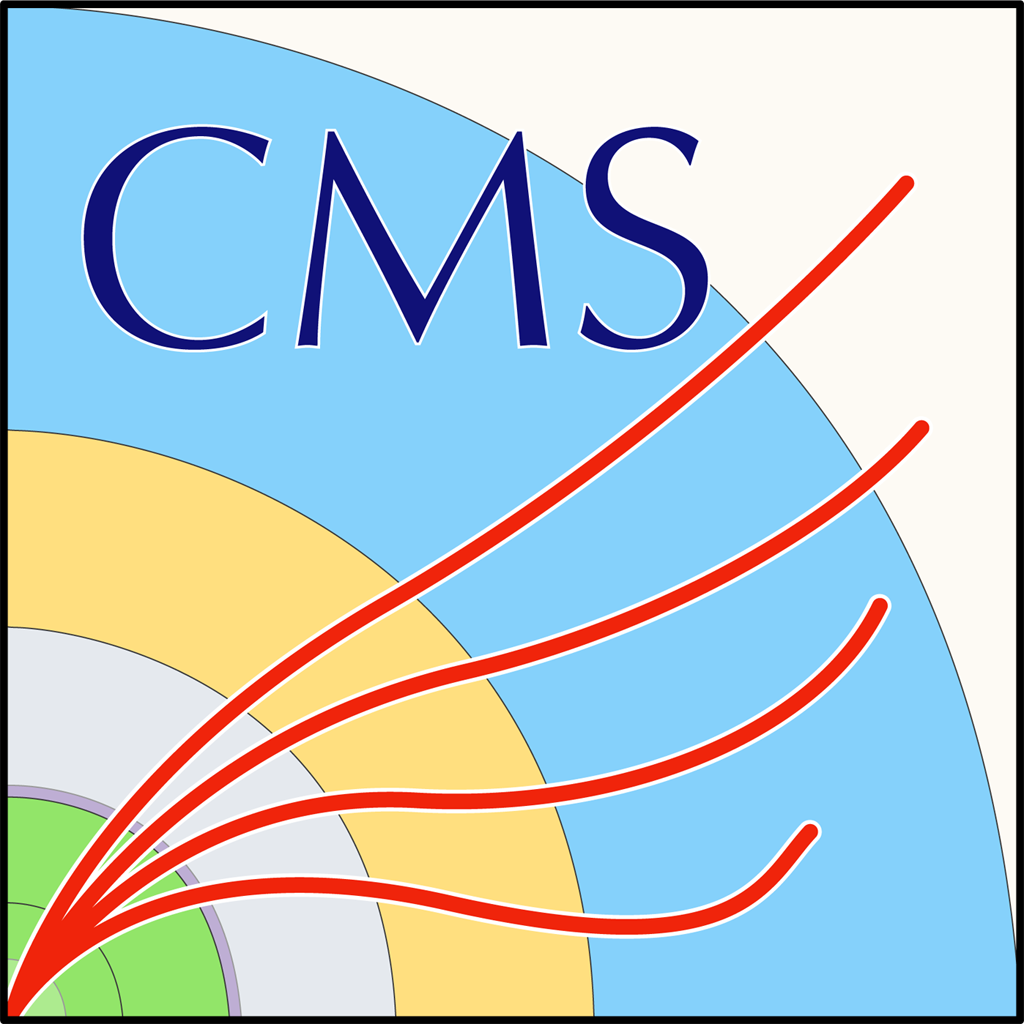
\includegraphics[width=0.052\textwidth]{slides/logos/logo_cms.png}
    \end{textblock*}}
    

% extra beamer settings
\AtBeginSection[]{\begin{frame}{Outline}\setcounter{tocdepth}{2}\tableofcontents[currentsection, hideothersubsections]\end{frame}}


% slides information
\title[\BWl measurement]{Measurement of W boson Branching Fraction in p-p Collisions at $\sqrt{s} = 13\TeV$  with the CMS Experiment}
\date{\today}
\author[Z. Chen]{Ziheng Chen}
\institute[NWU]{Department of Physics and Astronomy, \\ Northwestern University}
\addtobeamertemplate{title page}
{\centering \footnotesize {\color{NUpurple} Defence for the Ph.D. Degree in the Field of Physics  \rule{\linewidth}{0.2mm}} } 
{\centering \footnotesize \begin{center}  supervisor: Prof. Mayda Velasco  \end{center} }

    
\begin{document}
% title page
\begin{frame}{} \titlepage \end{frame}

% contents page
\begin{frame}{Outline}
\setcounter{tocdepth}{1}
\tableofcontents
    % \begin{columns}[t]
    %     \column{.5\textwidth}
    %     \tableofcontents[sections={1-3}]
    %     \column{.5\textwidth}
    %     \tableofcontents[sections={4-7}]
    % \end{columns}
\end{frame}


% sections
\section{Introduction}

% -------------
% new frame
% -------------
\begin{frame}{Introduction}
\smaller
    
    \begin{columns}
        \column{0.5\textwidth}
        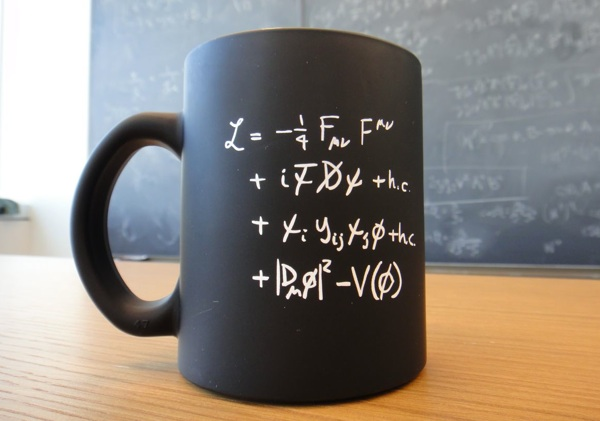
\includegraphics[width=\textwidth]{slides/figures/cernmug.jpeg}
        \column{0.5\textwidth}
        \begin{itemize} 
            \item The Standard Model (SM) represents the our current best understanding of the matter and force.
            \item It includes three generations of leptons (\Pe\PGne), (\PGm\PGnGm), (\PGt\PGnGt) and quarks (\PQu\PQd), (\PQc\PQs), (\PQt\PQb) as matter paticles, four gauge bosons \PGg, \PW, \PZ, \Pg as force particles, and one Higgs boson to generate mass.
            \item SM has been very successful in explaining and predicting experimental observations so far.
        \end{itemize}
    \end{columns}
    
    \vspace{0.05\textheight}
    \begin{itemize}
        \item The interaction between the leptons and \PW boson is encapsulated in the term $i\bar{\psi}\slashed{D}\psi$:
        \begin{equation*} \tiny
            i\bar{\psi}\slashed{D}\psi = 
            \bar{\chi}_L \gamma^\mu \big( i \partial_\mu  - \textcolor{red}{g} \frac{\tau_a}{2} W^a_\mu  -g'\frac{Y}{2} B_\mu \big) \chi_L 
            + \bar{\psi}_R \gamma^\mu \big( i \partial_\mu -g'\frac{Y}{2} B_\mu \big) \psi_R 
            - g_s (\bar{q}\gamma^\mu  T_{a} q) G_\mu^a 
        \end{equation*}
    \end{itemize}
\end{frame}



% -------------
% new frame
% -------------
\begin{frame}{Introduction}
\smaller 
    
    \begin{center}
    \resizebox{0.6\textwidth}{!}{    \feynmandiagram [inline=(d.base), small, horizontal=d to b] {
        a[particle=\PGne] -- [fermion] b [dot] -- [fermion] c[particle=\Pe], 
        b -- [boson, edge label=\PW] d,}; 
    = \qquad
    \feynmandiagram [inline=(d.base), small, horizontal=d to b] {
        a[particle=\PGnGm] -- [fermion] b [dot] -- [fermion] c[particle=\PGm],
        b -- [boson, edge label=\PW] d, }; 
    = \qquad
    \feynmandiagram [inline=(d.base), small, horizontal=d to b] {
        a[particle=\PGnGt] -- [fermion] b [dot] -- [fermion] c[particle=\PGt],
        b -- [boson, edge label=\PW] d,};}
    \end{center}
    
    \vspace{0.05\textheight}
    \begin{itemize} 
        \item One of the essential assumptions in SM is that the coupling strength $g$ is the same for all three generations of leptons, $g_\Pe = g_\PGm = g_\PGt \equiv g $, known as Lepton Universality (LU) in the weak interaction.
        \item Tests of the SM LU can be performed by studies of the leptonic decays of \PW bosons.
        \item In high-energy regime, the tests of lepton universality related to \PW boson have been performed on colliders.
        \begin{itemize} 
        \smaller 
            \item SPS and Tevatron using $\Pp\bar{\Pp}\to \PW$.
            \item LEP using $\Pe\bar{\Pe}\to \PW \PW$.
            \item LHC using $\Pp\Pp \to \PW$ and $\Pp\Pp \to \ttbar \to \PQb\PW \PAQb\PW$.
        \end{itemize}
        \item In low-energy regime, some of the most stringent LU tests come from the charge weak decays of mesons (e.g. \PD, \PB) and leptonic decays of taus~\cite{Amhis:2019ckw}. While most show high precision agreement with LU, tensions have been recently observed in the semileptonic decays of \PB mesons by Belle~\cite{Huschle:2015rga, Sato:2016svk, Hirose:2016wfn}, BaBar ~\cite{Lees:2012xj, Lees:2013uzd} and LHCb~\cite{Aaij:2015yra,Aaij:2017uff, Aaij:2017deq}.
    \end{itemize}
\end{frame}



% -------------
% new frame
% -------------
\begin{frame}{}
\smaller
    
    \begin{block}{SPS and Tevatron}
        \begin{columns}
            % add column
            \column{0.65\textwidth}
            \begin{itemize}
                \item the $\sigma_{\Pp\bar{\Pp}\to \PW} \times \BWl$ in three leptonic channels were measured by UA1~\cite{Albajar:1988ka}, UA2~\cite{appel1986measurement, Alitti:1991eh, Alitti:1992hv}, CDF~\cite{Abe:1990sd, Abe:1992ys, Abe:1991fb}, D0~\cite{Abbott:1999tt, Abazov:2003sv, Abachi:1995xc, Abbott:1999pk}.
                \item taus were reconstructed in the hadronic decay modes.
                \item Combined average $g^\PW_\PGt / g^\PW_\Pe = 0.988\pm 0.025$ were determined by \DZERO~\cite{Abbott:1999pk} consistent with SM.  
            \end{itemize}
            
            % add column
            \column{0.3\textwidth}
            \centering
            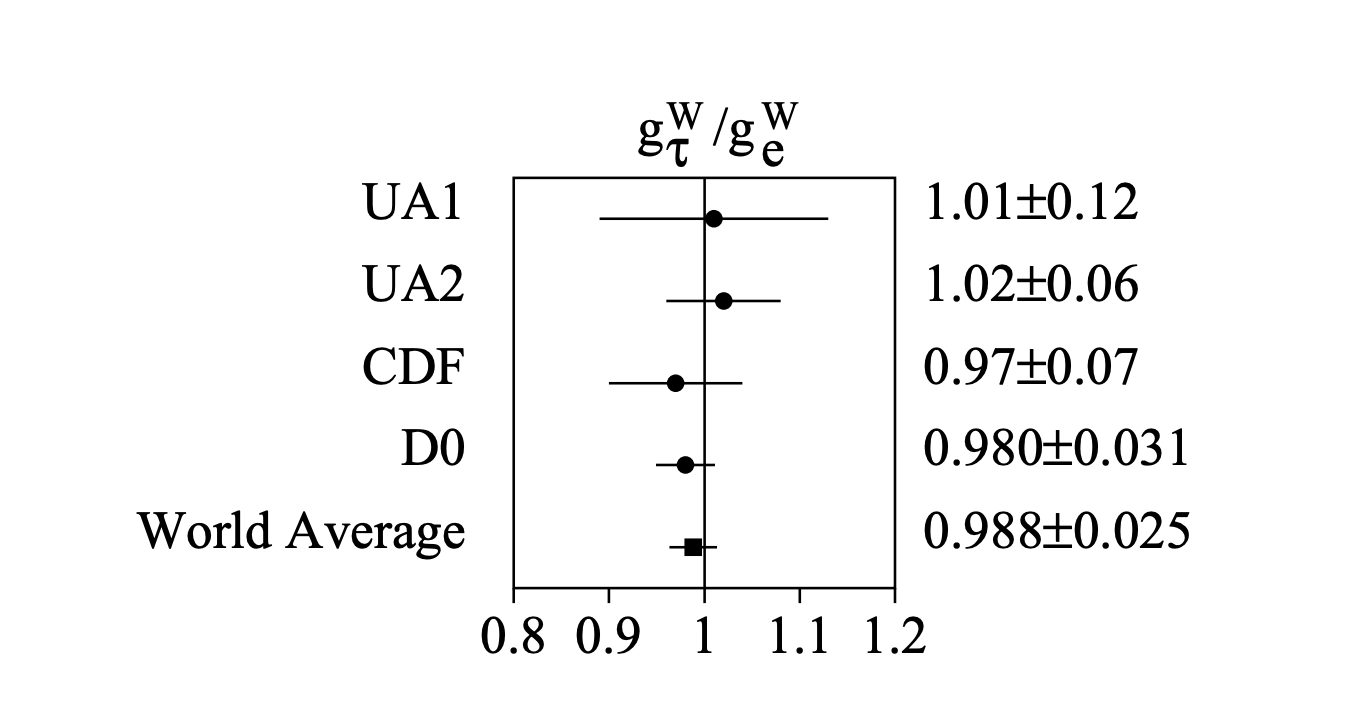
\includegraphics[width=\textwidth]{chapters/Introduction/sectionRelatedWorks/figures/spsTevatron.png}
        \end{columns}
    \end{block}
    
    \begin{block}{LEP-II}
        \begin{columns}
            % add column
            \column{0.65\textwidth}
            \begin{itemize}
                \item three individual leptonic \BWl were measured using pair-produced \WW from the electron-position collision by OPAL~\cite{Abbiendi:2007rs}, DELPHI~\cite{Abdallah:2003zm}, L3~\cite{Achard:2004zw}, ALEPH~\cite{Heister:2004wr}.
                \item the most precise and the only \BWl measurement available in PDG~\cite{pdg2020}.
                \item The LEP combined result~\cite{Schael:2013ita} showed agreement between electron and muon channel agree with each other, but tau channel was $2.6 \; \sigma$ above the average $$ \tiny 2\BWt/ \BWem = 1.066 \pm 0.025 $$ comparing with the SM prediction 0.999~\cite{Denner:1991kt,Rtau,dEnterria:2016rbf}.
            \end{itemize}
            
            % add column
            \column{0.3\textwidth}
            \centering
            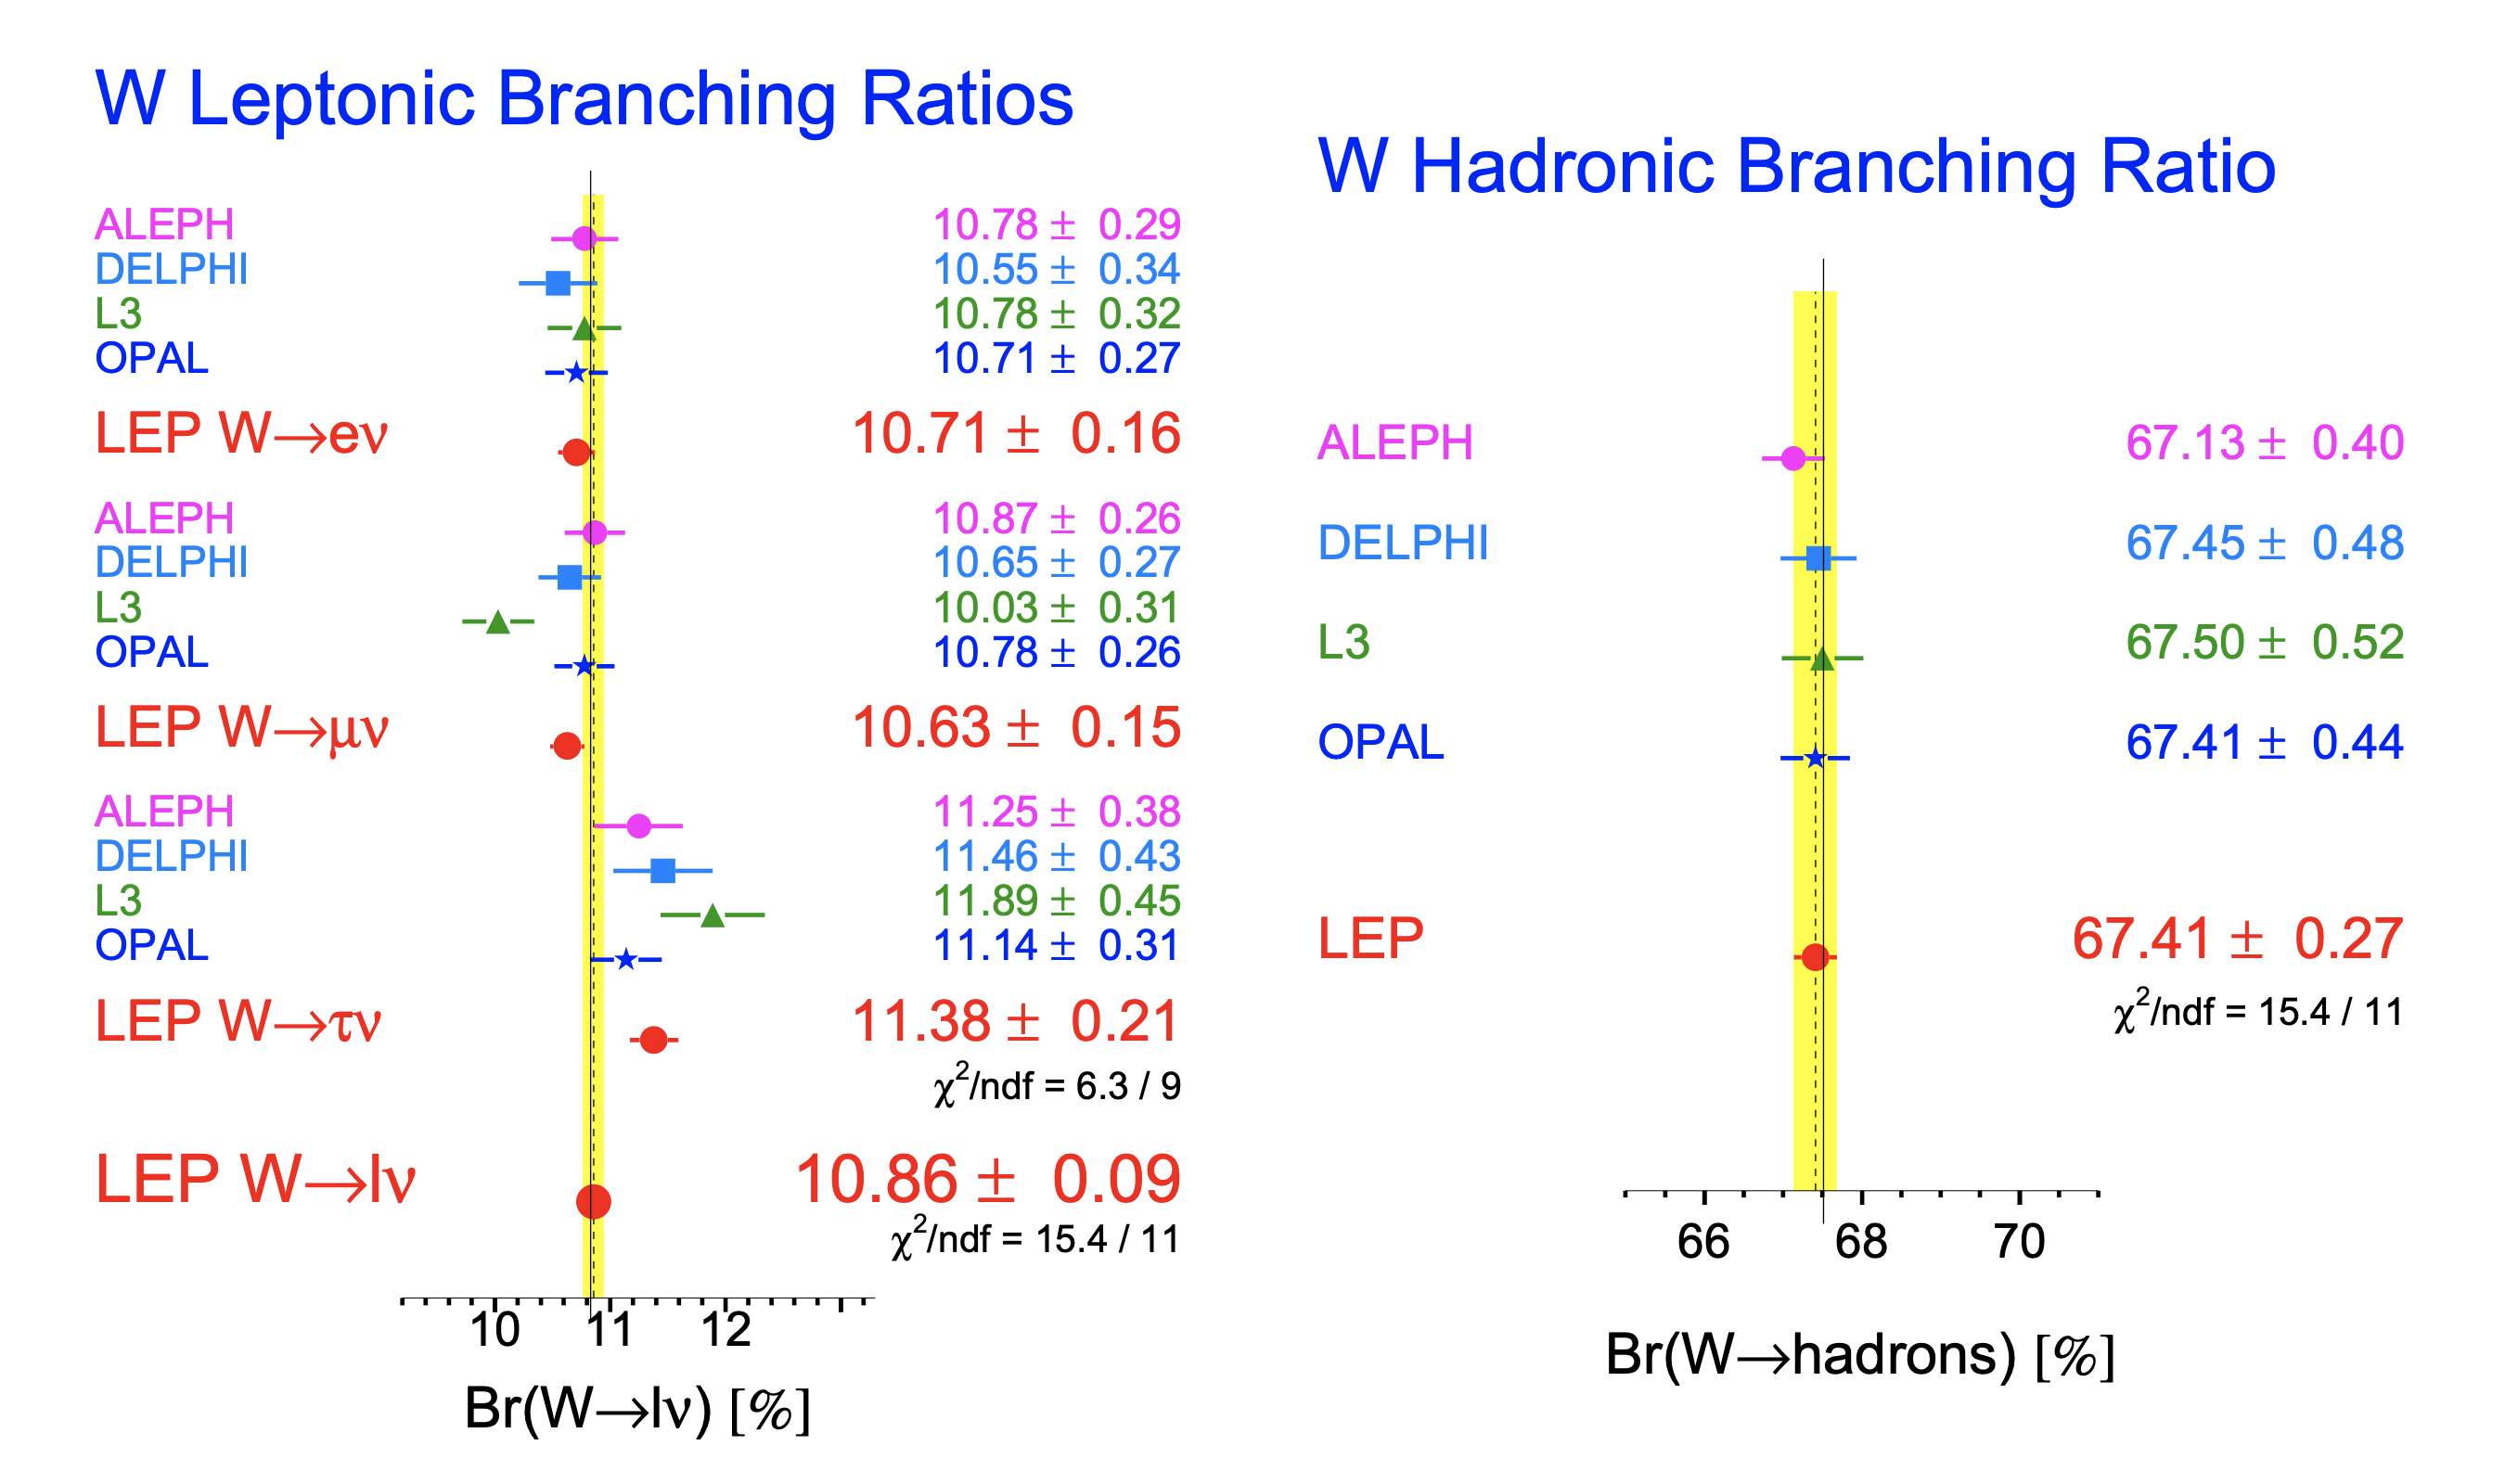
\includegraphics[width=\textwidth, trim=0 0 25cm 0, clip]{chapters/Introduction/sectionRelatedWorks/figures/lep.png}
        \end{columns}
    \end{block}
\end{frame}





% -------------
% new frame
% -------------
\begin{frame}{}
\smaller
    
    \begin{block}{LHC run-1}
        In the LHC run-1 at $\sqrt{s}=$ 7\TeV and 8\TeV, the LU between $\PW \to \Pe \PGn$ and $\PW \to \PGm \PGn$ has been tested by ATLAS~\cite{Aaboud:2016btc} and LHCb~\cite{Aaij:2015zlq, Aaij:2016qqz}.
        \begin{itemize}
            \item the \wjets cross-section was measured in electron and muon channels, ratio of which leads to $\BWm/\BWe$ as 1.003(10) by ATLAS and 0.980(18) by LHCb.
            \item the results agree with SM lepton universality.
        \end{itemize}
    \end{block}
                
   \begin{block}{LHC run-2}
        \begin{columns}[c]
            % add column
            \column{0.65\textwidth}           
            In the LHC run-2 at $\sqrt{s}=$ 13\TeV, ATLAS~\cite{Aad:2020ayz} has most recently published a test between muon and tau.
            \begin{itemize}
                \item use $\Pp\Pp\to\ttbar\to\PQb\PW\PAQb\PW$ events selected with \cmm, \cem plus two \PQb tagged jets final states.
                \item tau leptons are probed via muons from $\PGt\to\PGm\PAGnGm\PGnGt$, which tend to be softer and more displaced than prompt muons.
                \item fitting the transverse displacement and \pt of the probing muon leads to the ratio $$ \tiny \BWt/\BWm = 0.992 \pm 0.013 $$ consistent with the LU.
            \end{itemize}
            
            % add column
            \column{0.3\textwidth}
            \centering
            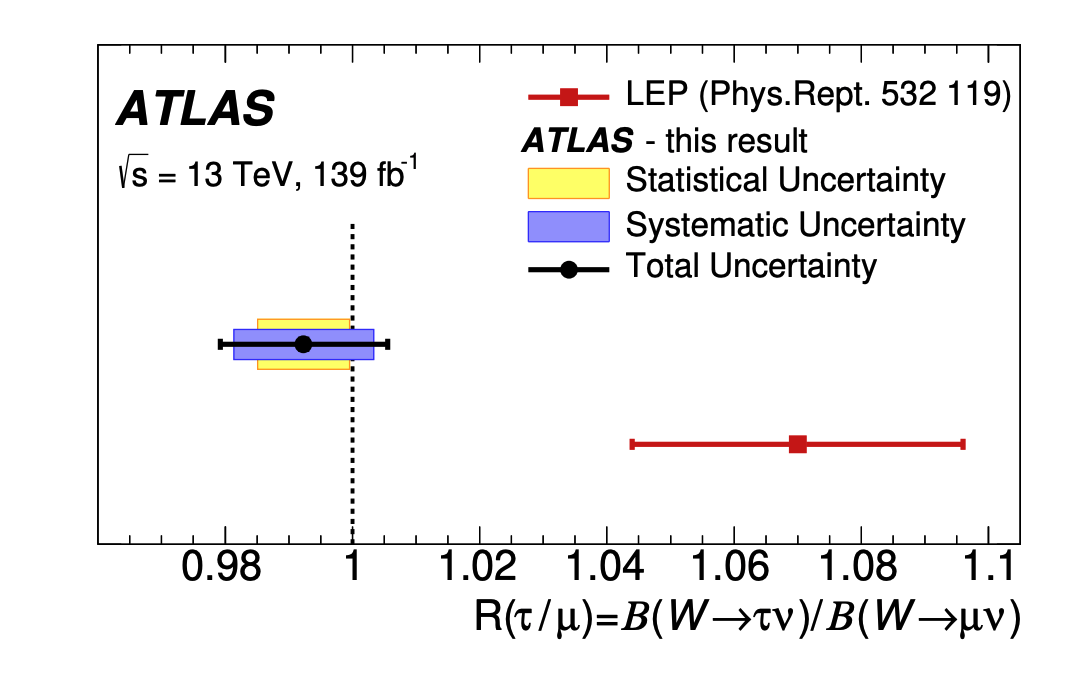
\includegraphics[width=\textwidth]{chapters/Introduction/sectionRelatedWorks/figures/atlas.png}
        \end{columns}
    \end{block}
\end{frame}






% -------------
% new frame
% -------------
\begin{frame}{}
\smaller
    \begin{columns}
        % add column
        \column{0.55\textwidth}
        \begin{block}{}
            \centering
            \small{\ttbar} process
            \resizebox{0.98\textwidth}{!}{    \feynmandiagram[small,horizontal=a to b]{
        i1 [particle=\PQq] -- [fermion] a -- [fermion] i2 [particle=\PQq],
        a -- [gluon, edge label=\Pg] b,
        f1 [particle=\PQt] -- [fermion] b -- [fermion] f2 [particle=\PQt],
        % top decay
        f1b[particle=\PQb] -- [fermion] f1 -- [photon] f1W [particle=\PW, red],
        f2b[particle=\PQb] -- [anti fermion] f2 -- [photon] f2W [particle=\PW, red],
        f1 -- [opacity=0.0] f2,
        f1W -- [opacity=0.0] f2W,
        f1b -- [opacity=0.0] f1W,
        f2b -- [opacity=0.0] f2W,
    }; \qquad
    \feynmandiagram[small,horizontal=a to b]{
        i1 [particle=\Pg] -- [gluon] a -- [gluon] i2 [particle=\Pg],
        a -- [gluon, edge label=\Pg] b,
        f1 [particle=\PQt] -- [fermion] b -- [fermion] f2 [particle=\PQt],
        % top decay
        f1b[particle=\PQb] -- [fermion] f1 -- [photon] f1W [particle=\PW, red],
        f2b[particle=\PQb] -- [anti fermion] f2 -- [photon] f2W [particle=\PW, red],
        f1 -- [opacity=0.0] f2,
        f1W -- [opacity=0.0] f2W,
        f1b -- [opacity=0.0] f1W,
        f2b -- [opacity=0.0] f2W,
    }; \qquad
    \feynmandiagram[small, vertical=a to b, horizontal=a to f1]{
        i1 [particle=\Pg] -- [gluon] a -- [anti fermion] f1 [particle=\PQt],
        a -- [fermion, edge label=\PQt] b,
        i2 [particle=\Pg] -- [gluon] b -- [fermion] f2 [particle=\PQt],
        % top decay
        f1b[particle=\PQb] -- [fermion] f1 -- [photon] f1W [particle=\PW, red],
        f2b[particle=\PQb] -- [anti fermion] f2 -- [photon] f2W [particle=\PW, red],
        f1 -- [opacity=0.0] f2,
        f1W -- [opacity=0.0] f2W,
        f1b -- [opacity=0.0] f1W,
        f2b -- [opacity=0.0] f2W,
        % i1 -- [opacity=0.0] i2,
        % f1 -- [opacity=0.0] f2,
    };}
        \end{block}
        % add column
        \column{0.4\textwidth}
        \begin{block}{}
            \centering
            \small{\tW} process
            \resizebox{0.98\textwidth}{!}{    \feynmandiagram[scale=0.7][horizontal=a to b]{
        i1 [particle=\PQb] -- [fermion] a -- [gluon] i2 [particle=\Pg],
        a -- [fermion, edge label=\PQb] b,
        f1 [particle=\PW , red] -- [photon] b -- [fermion] f2 [particle=\PQt],
        f2b[particle=\PQb] -- [anti fermion] f2 -- [photon] f2W [particle=\PW, red],
        f1 -- [opacity=0.0] f2W,
    }; \qquad
    \feynmandiagram[scale=0.7][vertical=a to b]{
        i1 [particle=\PQb] -- [fermion] a -- [photon] f1 [particle=\PW, red],
        a -- [fermion, edge label=\PQb] b,
        i2 [particle=\Pg] -- [gluon] b -- [fermion] f2 [particle=\PQt],
        f2b[particle=\PQb] -- [anti fermion] f2 -- [photon] f2W [particle=\PW, red],
        i1 -- [opacity=0.0] i2,
        f1 -- [opacity=0.0] f2W -- [opacity=0.0] f2b,
    };}
        \end{block}
    \end{columns}
    
    \vspace{0.1\textheight}
    \begin{itemize}
        \item This analysis presents a CMS measurement of three individual \BWl and a test of lepton universality in the \PW decay, 
        \begin{itemize} 
        \smaller
            \item use the run 2016 dataset from the LHC $\sqrt{s}=13\TeV$ proton-proton collisions.
            \item treat \ttbar and \tW processes as the primary signals.
        \end{itemize}       
        \item Motivations
        \begin{itemize} 
        \smaller
            \item The measurements of three \PW leptonic branching fractions have not been improved for more than a decay since LEP;
            \item LEP's $R_{\PGt/(e,\PGm)}$ shows a $2.6\,\sigma$ deviation from the SM prediction.
        \end{itemize}
        \item Opportunities
        \begin{itemize} 
        \smaller
            \item LHC 13\TeV \Pp-\Pp collisions produce a large number of \ttbar events giving $\PW\PW$ pairs;
            \item The improved \PQb tagging allows to select \ttbar events with a high purity;
            \item The improved \PGth identification enables to efficiently select \PW tauonic decays.
        \end{itemize}
    \end{itemize}
\end{frame}
    
    
    
    
    
% \begin{frame}{Introduction}
%     \begin{center}
%     \begin{itemize} \smaller
%         \item A
%         \item B
%     \end{itemize}
%     \end{center}
    
%     \begin{center}
%     \begin{columns}
%         % add column
%         \column{0.4\textwidth}
%         add column
        
%         % add column
%         \column{0.6\textwidth}
%         add column
%     \end{columns}
%     \end{center}
% \end{frame}
    

            

        


\section{The CMS and Tau Reconstruction}
\begin{frame}{CMS Detector}
    \begin{center}
        \includegraphics[width=0.9\textwidth]{chapters/CMSExperiment/sectionDetector/figures/cmsDetector.png}
    \end{center}
\end{frame}



%

\begin{frame}{}
\smaller
    \begin{columns}
    \column{0.6\textwidth}

    \begin{itemize} 
        \item Brain of the detector: Two-level trigger system.
        \item level-1 trigger (L1T)
        \begin{itemize} 
            \item customized ASICs and onsite FPGAs
            \item consider muon chamber and calorimeter
            \item 40MHz to 100kHz
            \item comprised of local, regional and global 
            \item latency budget 4\mus 
        \end{itemize}
        
        \item high-level trigger (HLT)
        \begin{itemize} 
            \item CPU. commodity computers of builder-filter.
            \item run a streamlined version of offline reconstruction software, filter with a HLT menu
            \item 100\;kHz to 1\;kHz
            \item in 2012, 13000 CPU cores 200 ms/event \cite{Trocino:2014jya}
        \end{itemize}
    \end{itemize}
    
    
    \column{0.4\textwidth}
    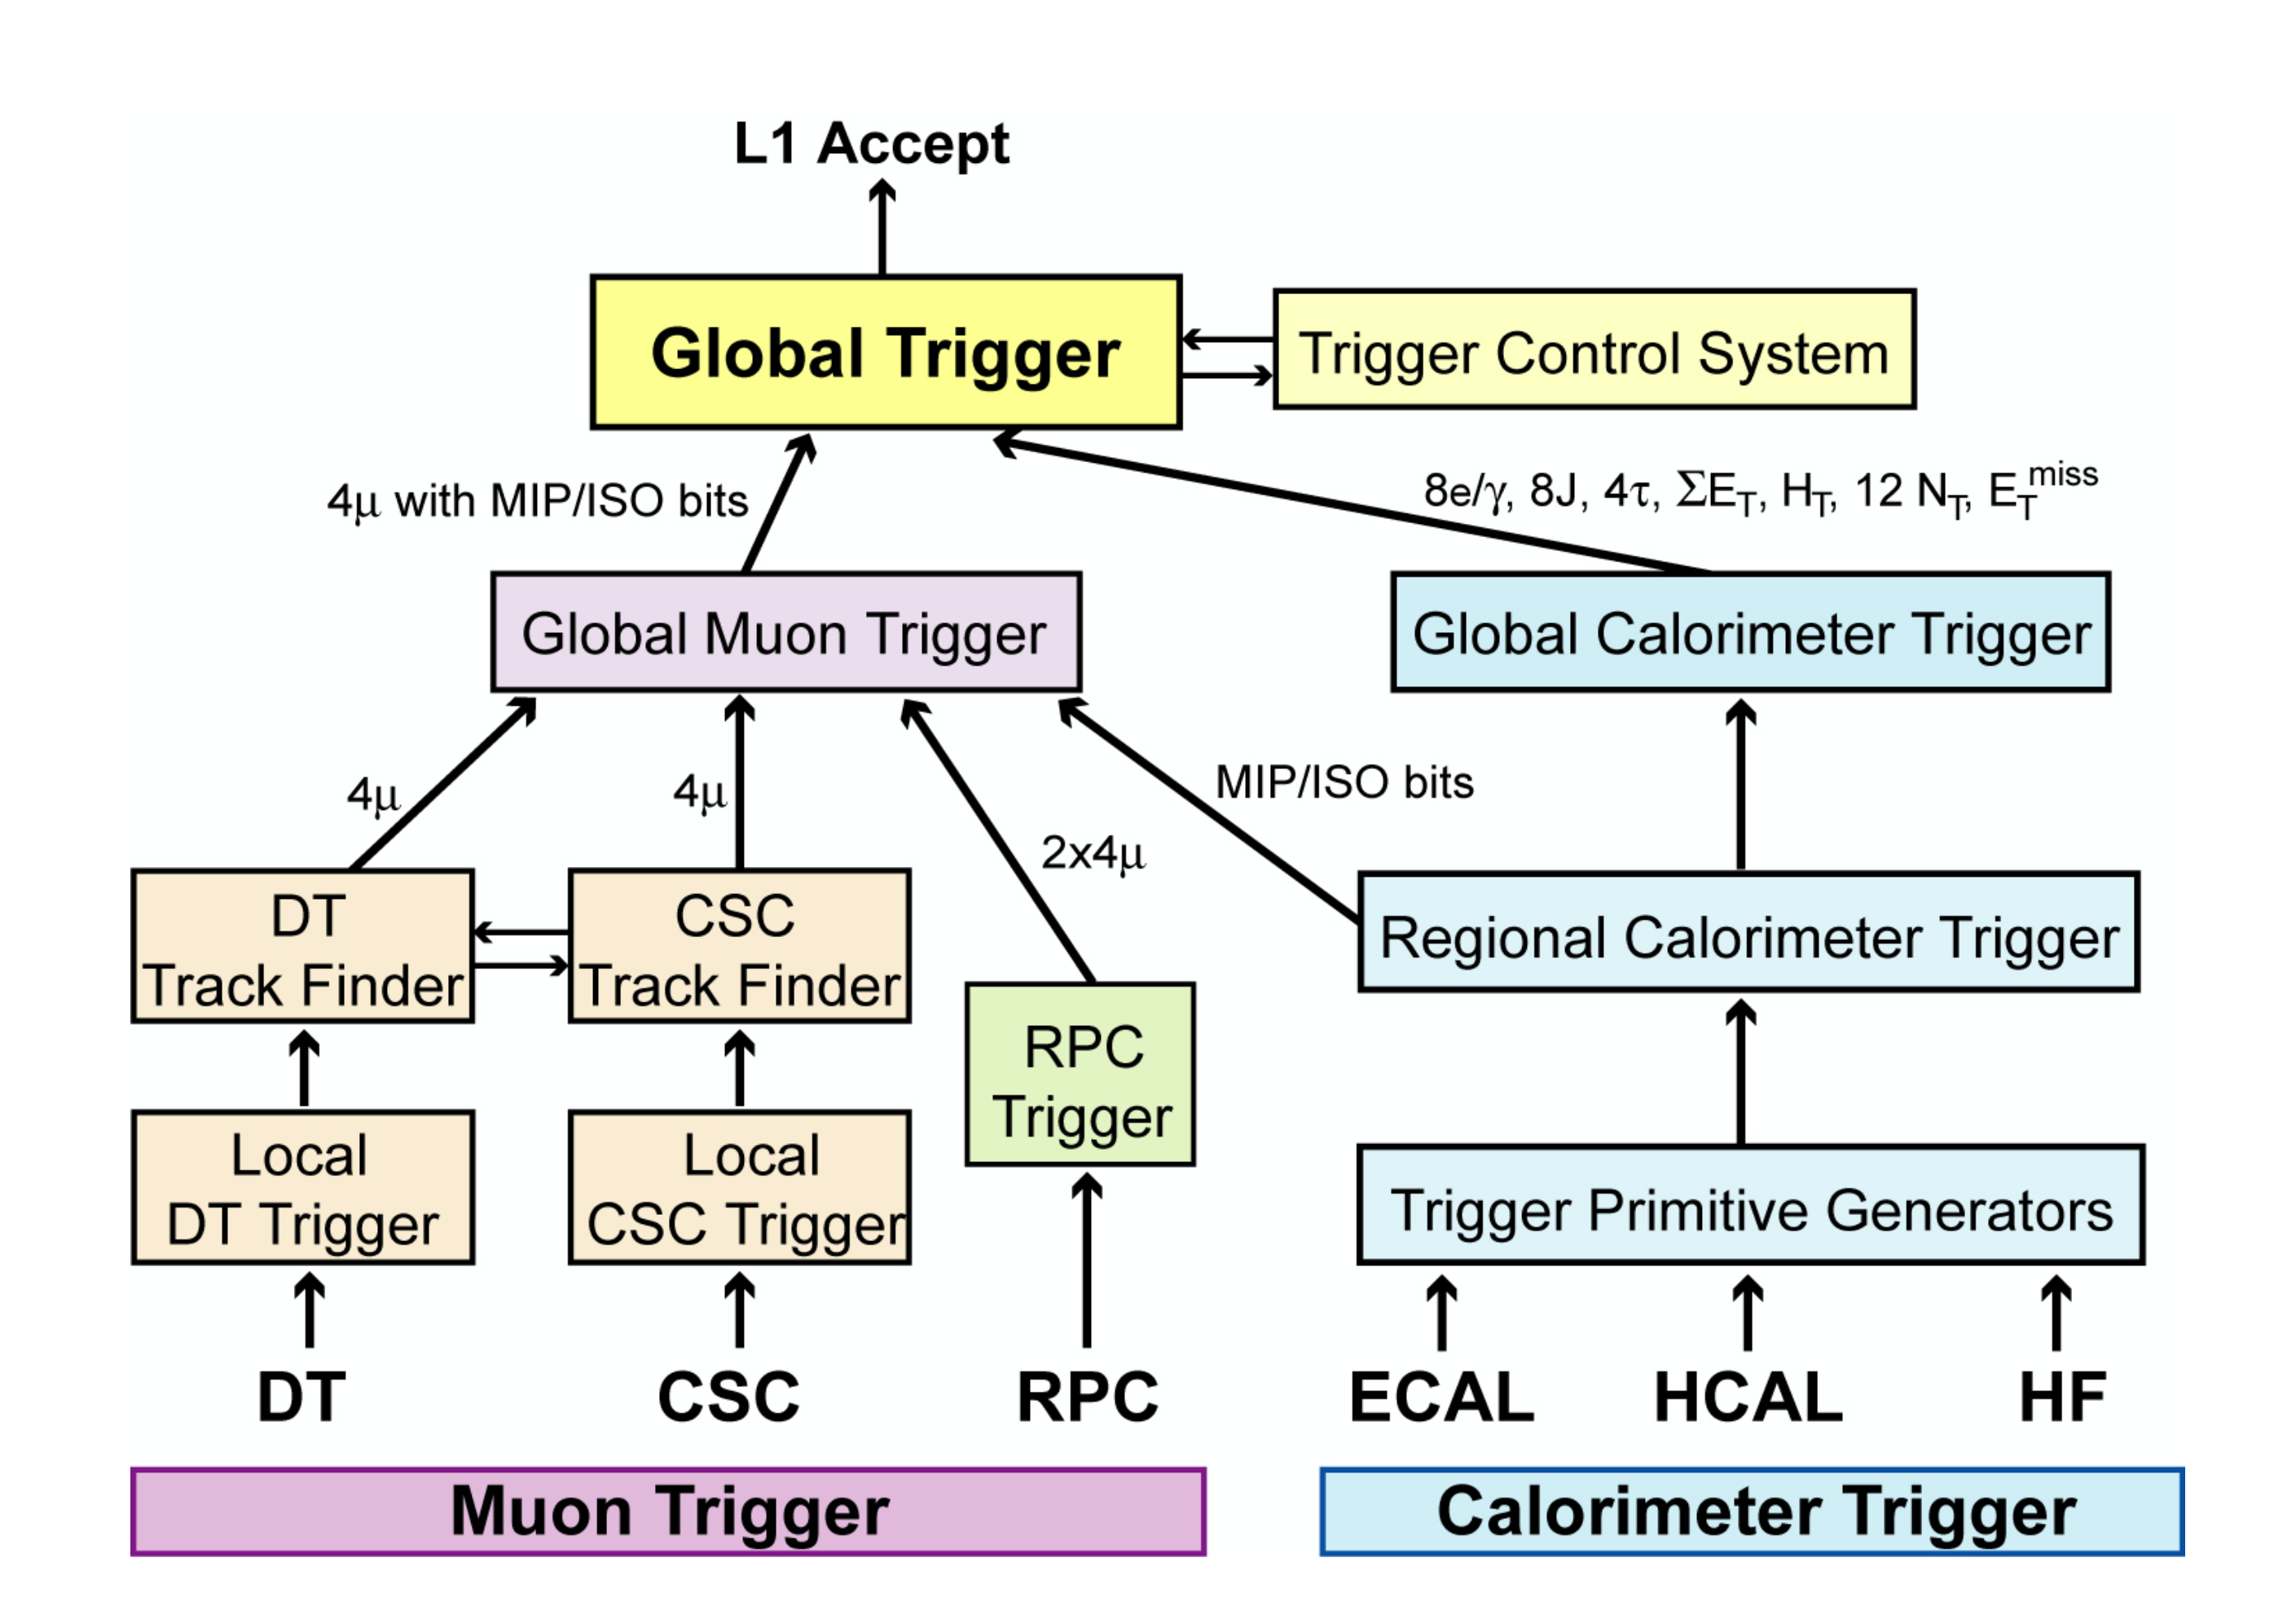
\includegraphics[width=\textwidth]{chapters/CMSExperiment/sectionTrigger/figures/trigger.png}
    \end{columns}
\end{frame}


\begin{frame}{CMS Detector}
    \begin{center}
        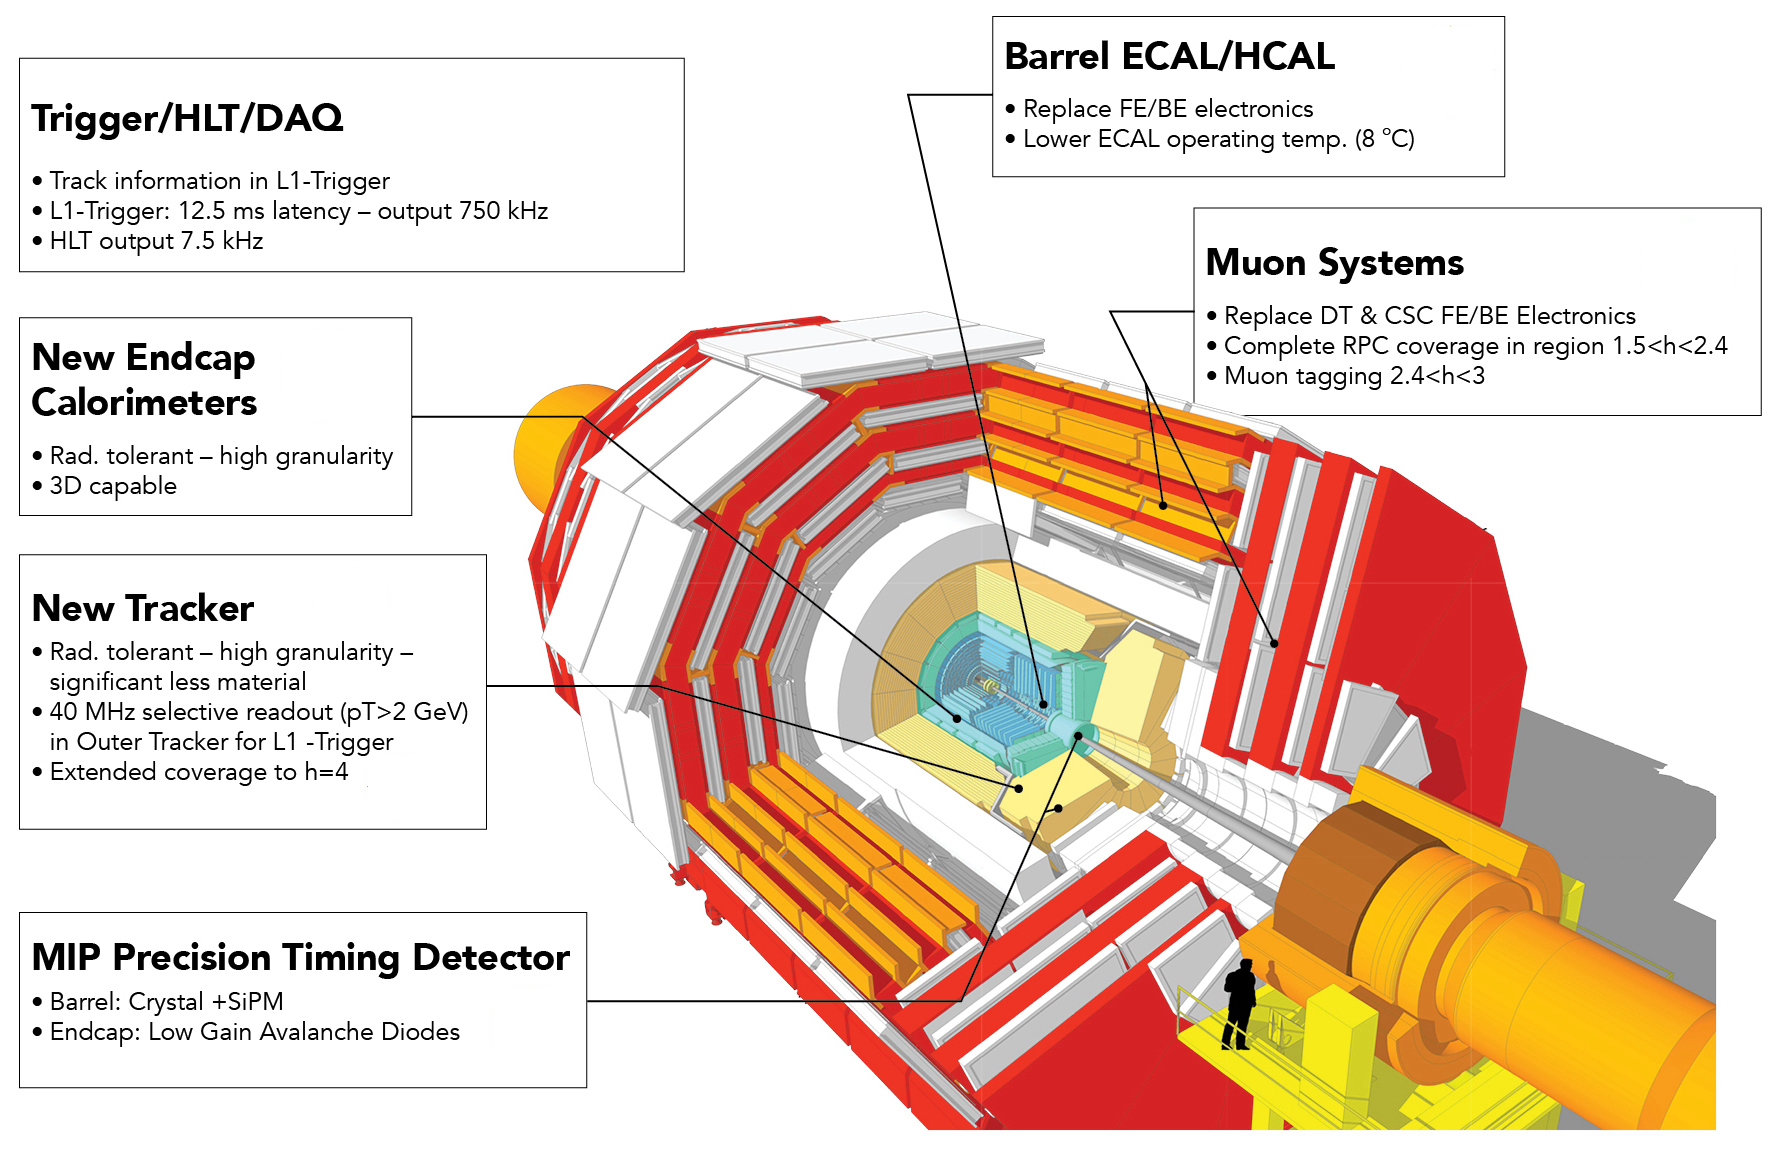
\includegraphics[width=0.9\textwidth]{slides/figures/CMS_NSF_DOE.jpeg}
    \end{center}
    \footnote{ https://www.classe.cornell.edu/NewsAndEvents/CLASSENewsCMS180129Ryan.html}
\end{frame}




\begin{frame}{Particle-Flow Reconstruction}
\smaller
    \begin{center}
        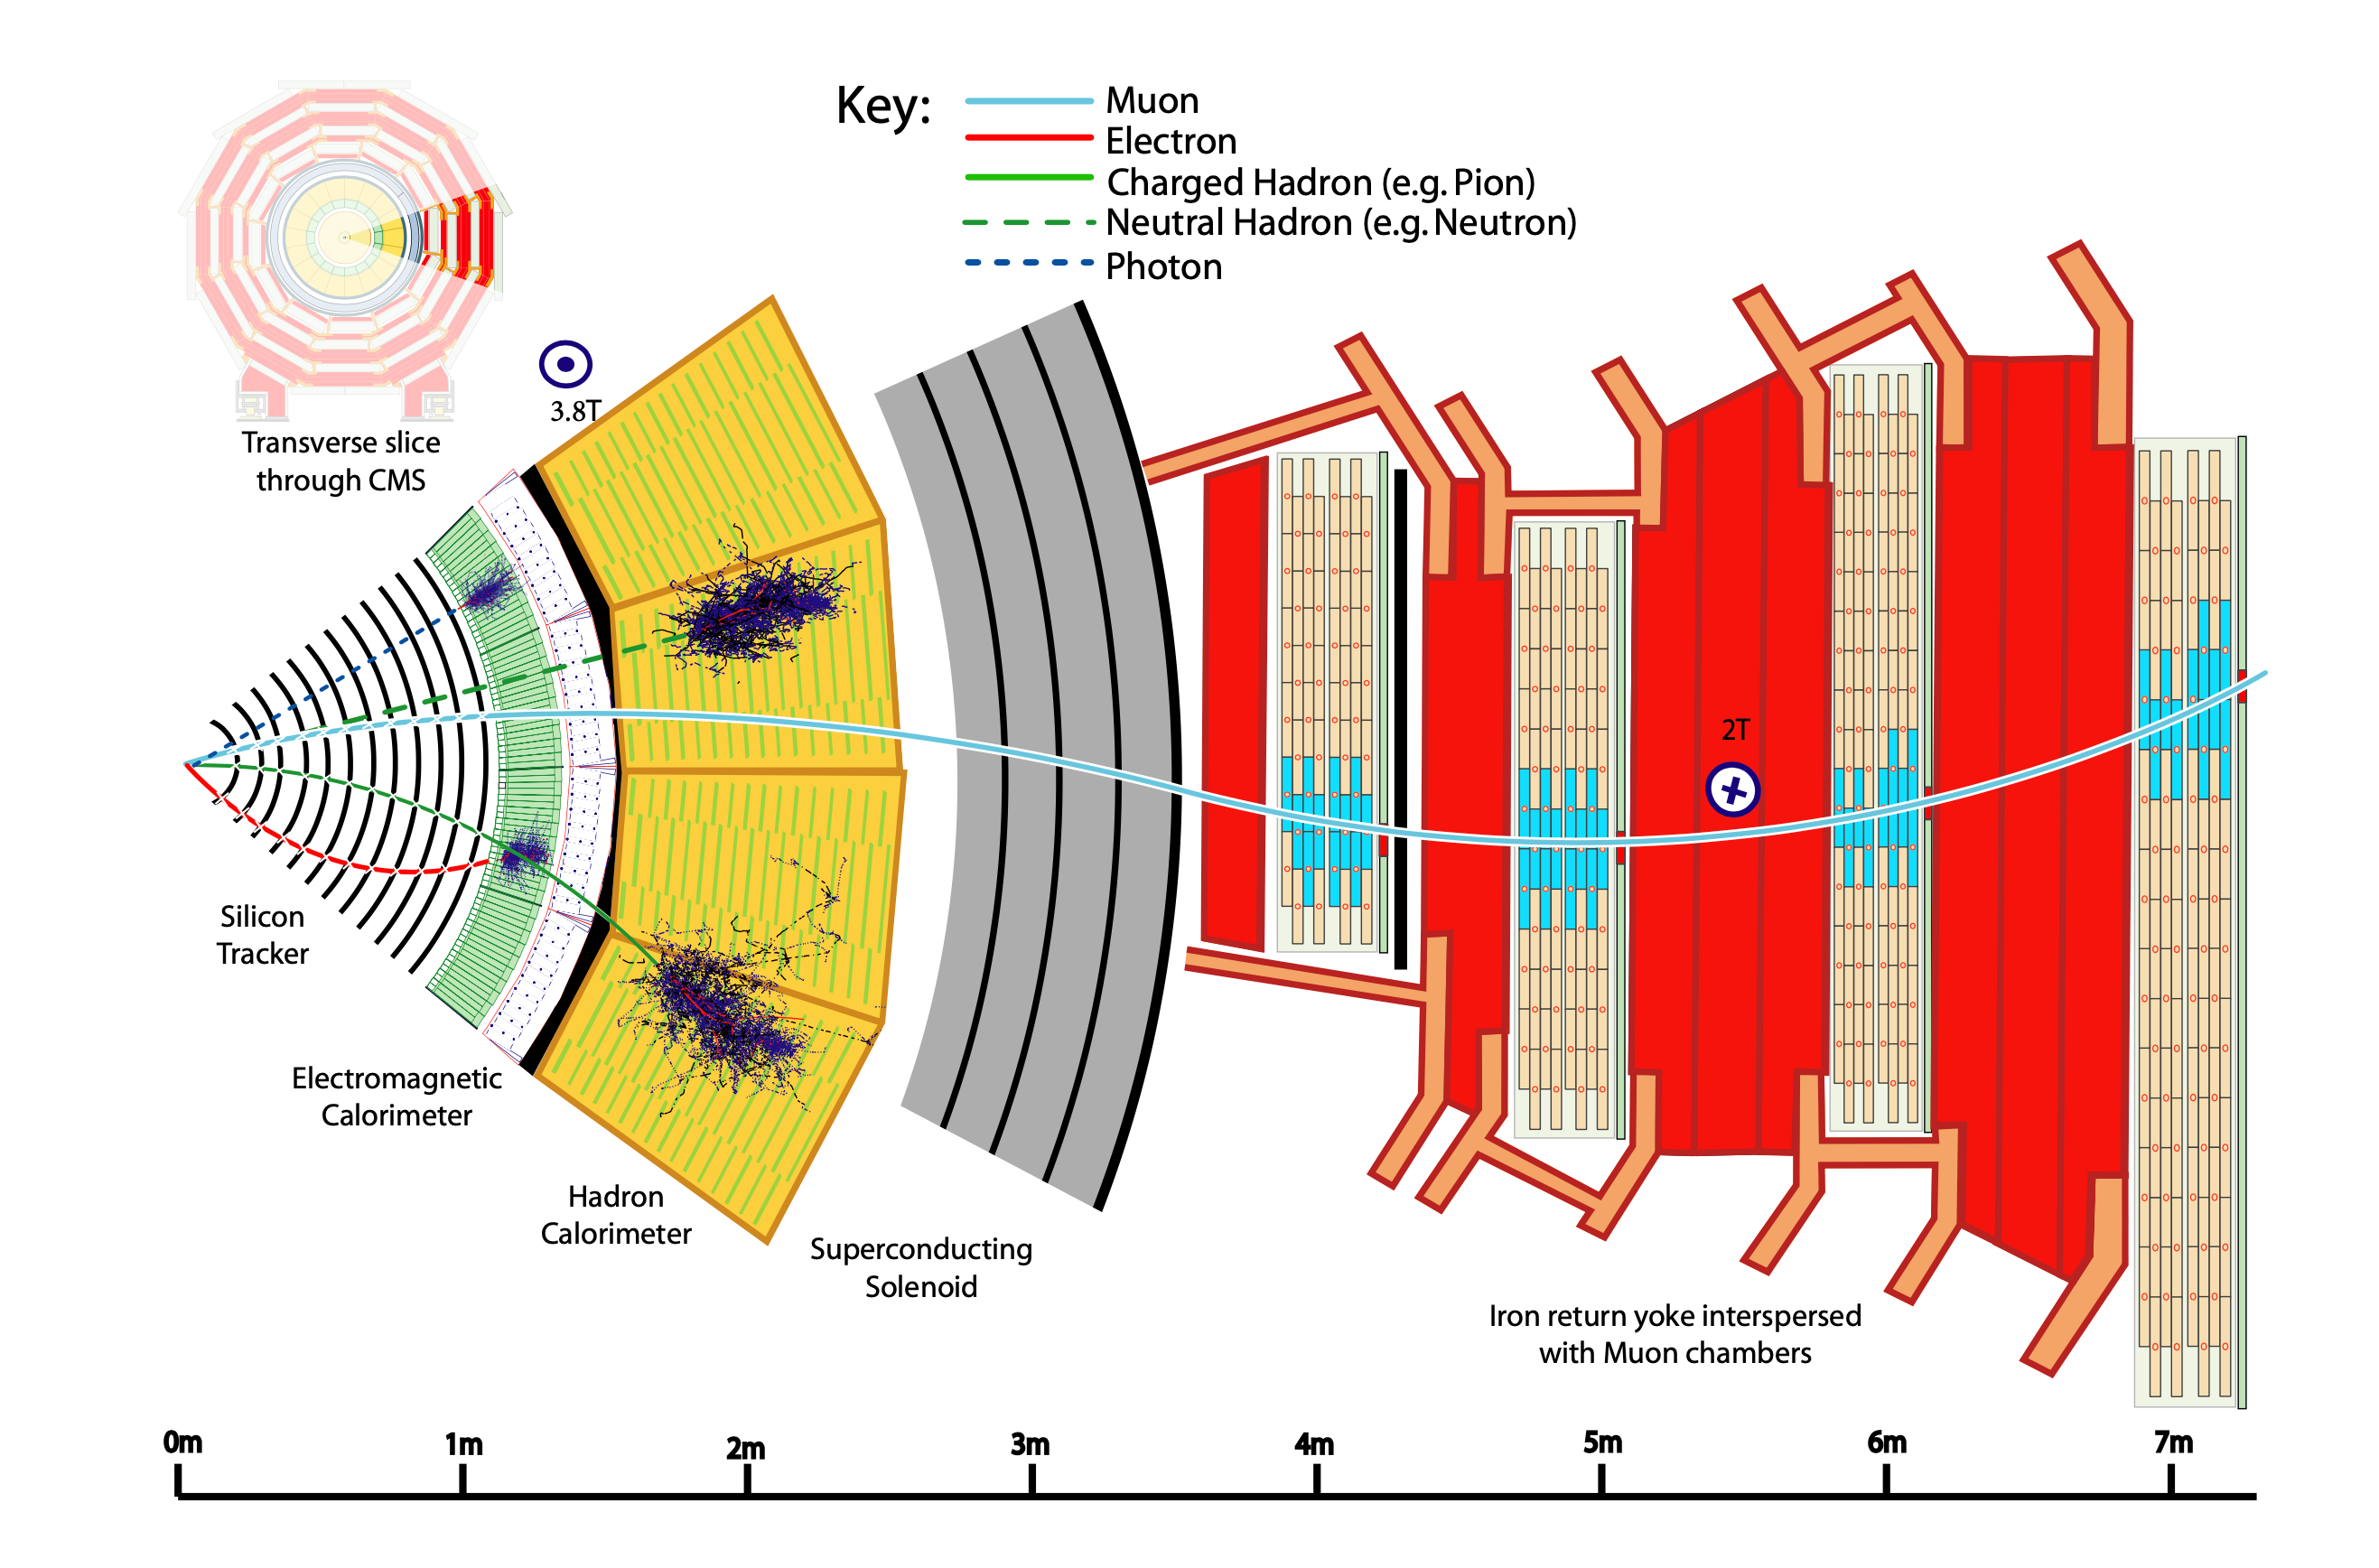
\includegraphics[width=0.7\textwidth]{chapters/CMSExperiment/sectionReconstruction/figures/pfa.png}
    \end{center}
    \begin{itemize} 
        \item combines information in all subdetector to construct final state particles (called PF candidate) muon, electron, charged hadron, neutral hadron, photon.
        \item main steps PF blocks, linking, identification/energy regression.
        \item Jets are clustered by anti-\kt based on PF candidates. 
    \end{itemize}
\end{frame}

\begin{frame}{Hadronic Tau Reconstruction}
\smaller
    \begin{center}
        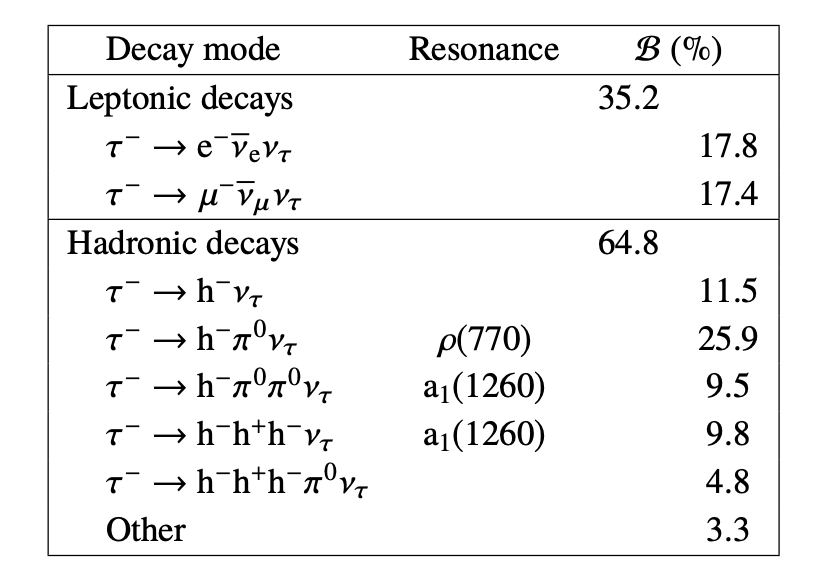
\includegraphics[width=0.5\textwidth]{slides/figures/tauDecay.png}
    \end{center}
    \begin{block}{Tau Property}
    \begin{itemize} 
        \item mass $m_\PGt = 1.776\GeV$ and lifetime $c\Gamma = 87\mum$
        \item 65\% decay hadronically
        \item fixed pattern of final-state particles
        \item defined visible mass at $\rho (770)$ and $a_1(1260)$
    \end{itemize}  
    \end{block}
\end{frame}

\begin{frame}{}
\smaller
    \begin{center}
        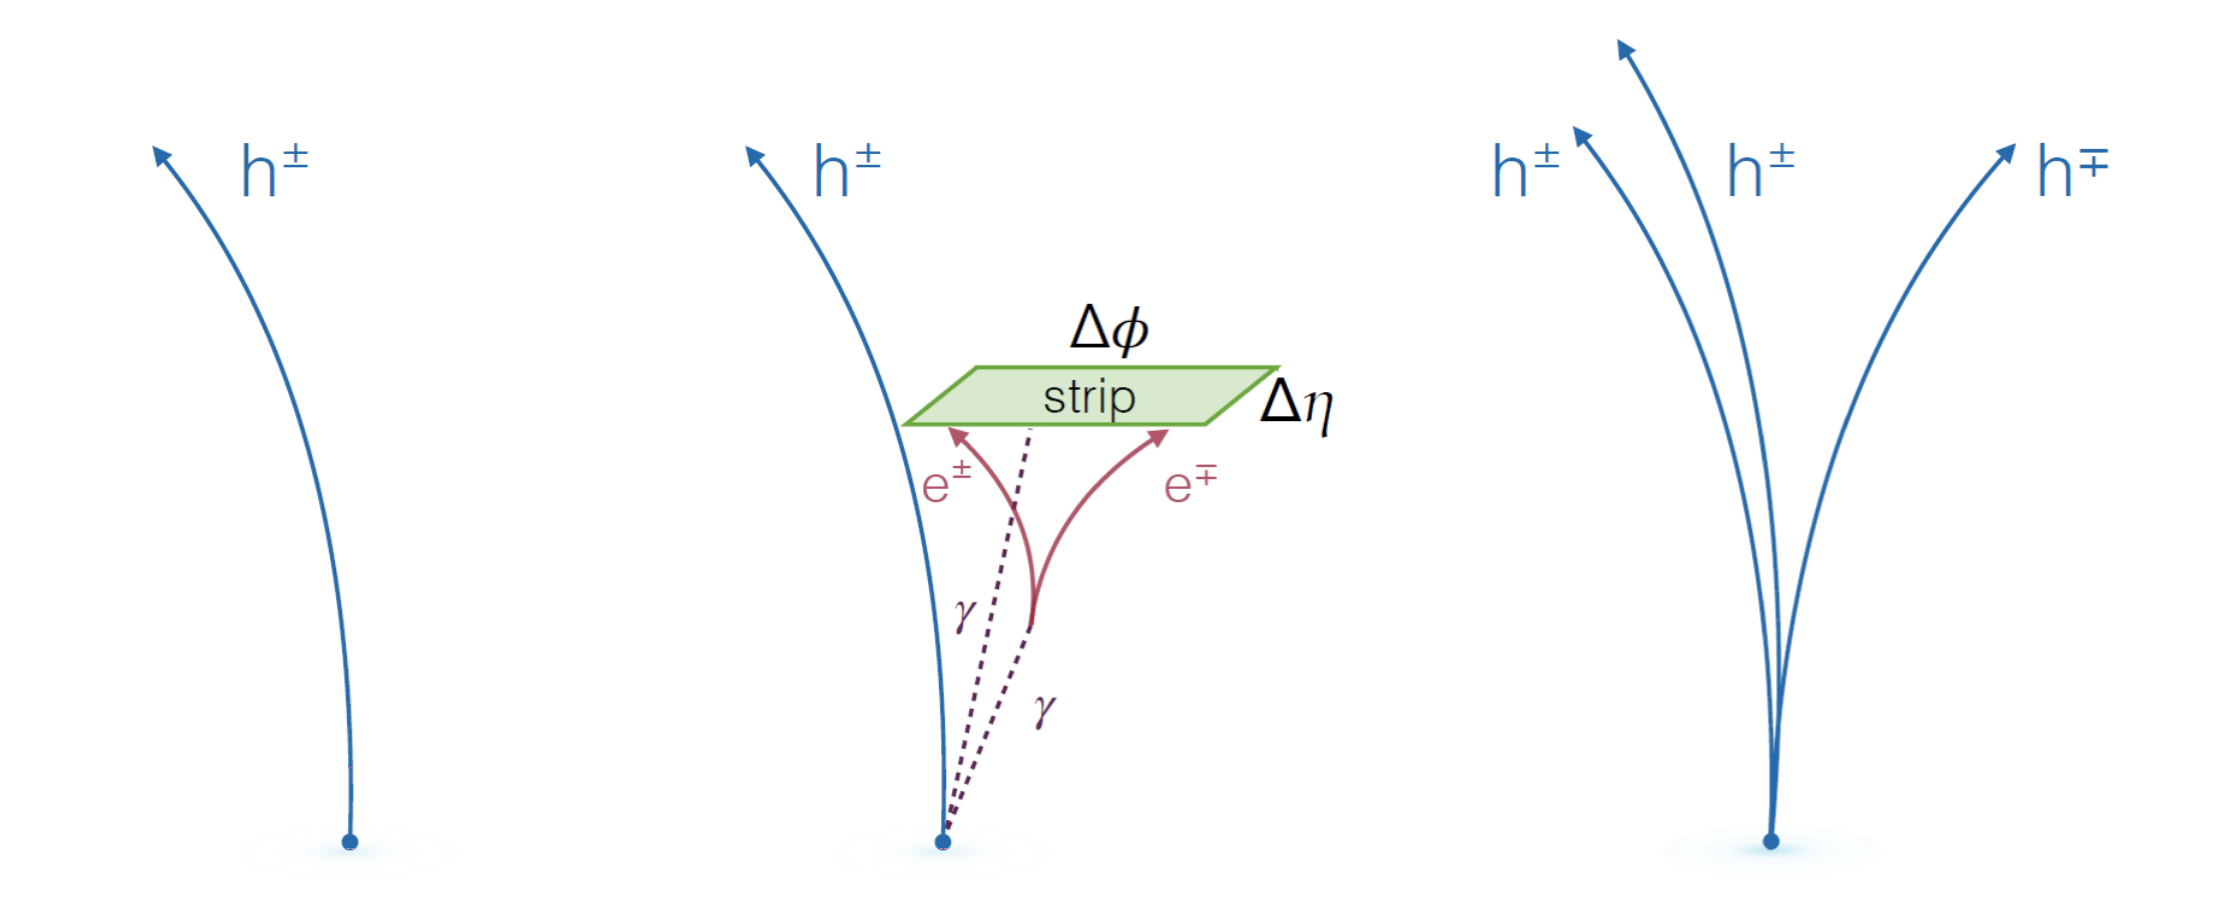
\includegraphics[width=0.6\textwidth]{slides/figures/tauReco.png}
    \end{center}
    \begin{block}{Hadrons-plus-strips (HPS)}
    Taus are reconstructed in their hadronic modes with Hadrons-plus-strips (HPS) algorithm from tagging PF jets
    \begin{itemize} 
        \item cluster \Pe/\PGg into strips. merging \Pe/\PGg in \pt decreasing order with a dynamic window size $\Delta\eta \times \Delta \phi = 0.20\pt^{-0.66} \times 0.35 \pt^{-0.71}$ 
        \item select charged hadrons (prong) $\pt>0.5\GeV$ and $d_{xy}<0.1$~cm.
        \item match to combination of hadrons and strips to \PGth decay modes.
        \item veto when
        \begin{itemize} 
        \smaller
            \item visible mass not competent with expected $\rho (770)$ and $a_1(1260)$ resonance
            \item not single charged
            \item any component falls outside signal cone $\Delta R_{sig} = \frac{3.0 \text{ GeV } } { \pt (\text{ hadronic system})  }$, with $0.05 \leq \Delta R_{sig} \leq 0.1.$
        \end{itemize}
    \end{itemize}  
    \end{block}
\end{frame}


\begin{frame}{Hadronic Tau Reconstruction}
\smaller
    
    \begin{columns}[c]
        \column{0.6\textwidth}
        \begin{block}{Discriminate against contamination}
        \begin{itemize} 
            \item discriminate against quark and gluon jets.
            \item iso-based discriminator: 
            \begin{itemize} 
            \smaller
                \item isolation is calculated energy sum in the ring between signal cone and $\Delta R = 0.3$ cone.
                \item quark and gluon jets tend to have larger isolation, while tau jets tend to have smaller.
            \end{itemize}
        
             
            % \begin{equation}
            % \tiny
            %     I_{\PGth} = \sum \pt^{\text{charged}} (d_z<0.2 \text{cm}) + \max \bigg( 0, \sum \pt^ \PGg - \Delta \beta \sum \pt^{\text{charged}} (d_z>0.2 \text{cm})  \bigg )
            % \end{equation}
            
            \item MVA-based discriminator: 
            \begin{itemize} 
            \smaller
                \item combine isolation and other variables sensitives to tau lifetime (e.g. SIP3D, d0).
                \item use boosted decision tree (BDT)
            \end{itemize}
        \end{itemize}
        \end{block}

        \column{0.4\textwidth}
        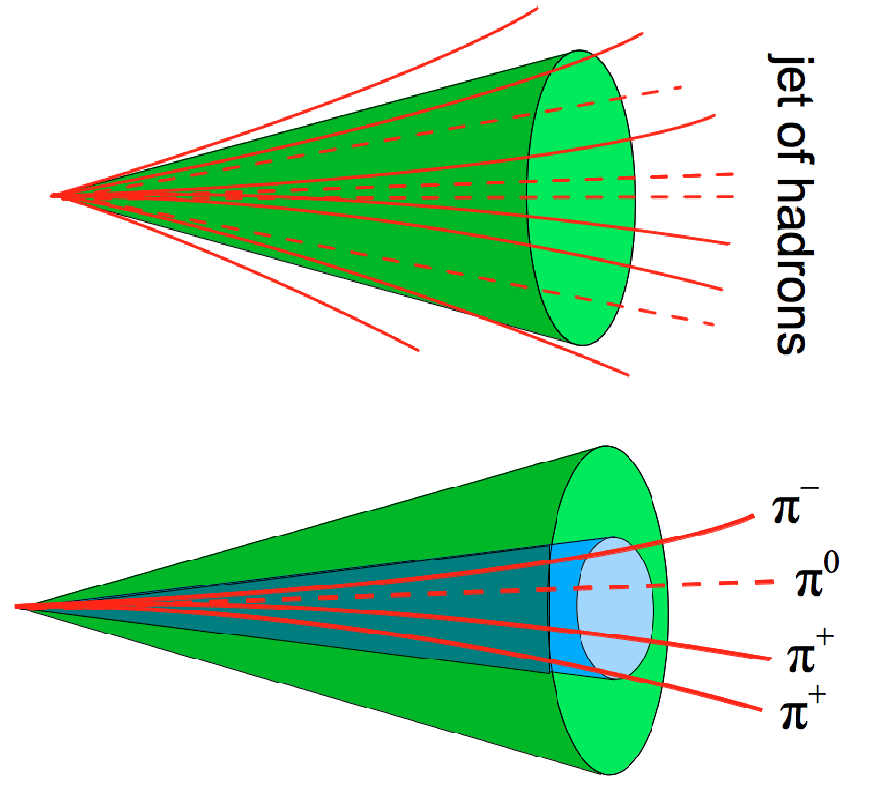
\includegraphics[width=\textwidth]{slides/figures/tausignature_trans.png}
    \end{columns}
    
\end{frame}
\section{Selections}


\subsection{Event selections}

\begin{frame}{Event selection}
\smaller
    \begin{table}
        \centering
        \setlength{\tabcolsep}{1em}
        \renewcommand{\arraystretch}{1.5}
        \resizebox{0.95\textwidth}{!}{    \begin{tabular}{c|c|ccc|c|c}     
        \hline 
        trigger                & label  & $N_{\Pe}$ & $N_{\PGm}$ & $N_{\PGt}$   & \pt & other  \\
        \hline                                                                                      
        \multirow{4}{*}{\Pe}   & \cee   & 2         & 0          & 0            & $\pt^{\Pe(\Pe)}  > 30 \, (20)\GeV$ & OS, $|m_{\cee} - m_{\PZ}| > 15\GeV$   \\
                               & \cem   & 1         & 1          & 0            & $\pt^{\Pe(\PGm)} > 30 \, (10)\GeV$ & OS\\
                               & \cet   & 1         & 0          & 1            & $\pt^{\Pe(\PGth)}> 30 \, (20)\GeV$ & OS\\
                               & \ceh   & 1         & 0          & 0            & $\pt^{\Pe} > 30\GeV$               &    \\
        \hline                                                                      
        \multirow{4}{*}{\PGm}  & \cme   & 1         & 1          & 0            & $\pt^{\PGm(\Pe)}  > 25 \, (20)\GeV$ & OS \\
                               & \cmm   & 0         & 2          & 0            & $\pt^{\PGm(\PGm)} > 25 \, (10)\GeV$ & OS,$|m_{\cmm} - m_{\PZ}| > 15\GeV$  \\
                               & \cmt   & 0         & 1          & 1            & $\pt^{\PGm(\PGth)}> 25 \, (20)\GeV$ & OS \\
                               & \cmh   & 0         & 1          & 0            & $\pt^{\PGm} > 25\GeV$               &    \\\hline 
                        
    \end{tabular}}
    \end{table}
    % \small{ *) opposite sign (OS)}
    
    \begin{itemize}
        \item Channels are further split based on $n_j$ and $n_b$
        \item Baseline categories require
        \begin{itemize}
        \smaller
            \item $n_j\geq 2$ in $\ell\ell$ and $\ell \PGth$ channels,
            \item $n_j\geq 4$ in \ceh and \cmh channels,
        \end{itemize}
        with either $n_b=1$ or $n_b\geq2$, giving a high purity of \ttbar and \tW.
    \end{itemize}
    
    \footnotetext[1]{\tiny OS for opposite sign.}
    \footnotetext[2]{\tiny counting analysis uses $\pt^\PGm>30 \GeV$ for the leading muon in muon triggered channels to reduce QCD.}
\end{frame}




\begin{frame}{}
    Baseline categories with $n_b=1$
    \begin{block}{\smaller \PGm trigger}
    \begin{center}
        \centering
        \cme \qquad\qquad\qquad\quad \cmm \qquad\qquad\qquad\quad \cmt \qquad\qquad\qquad\quad \cmh \\
        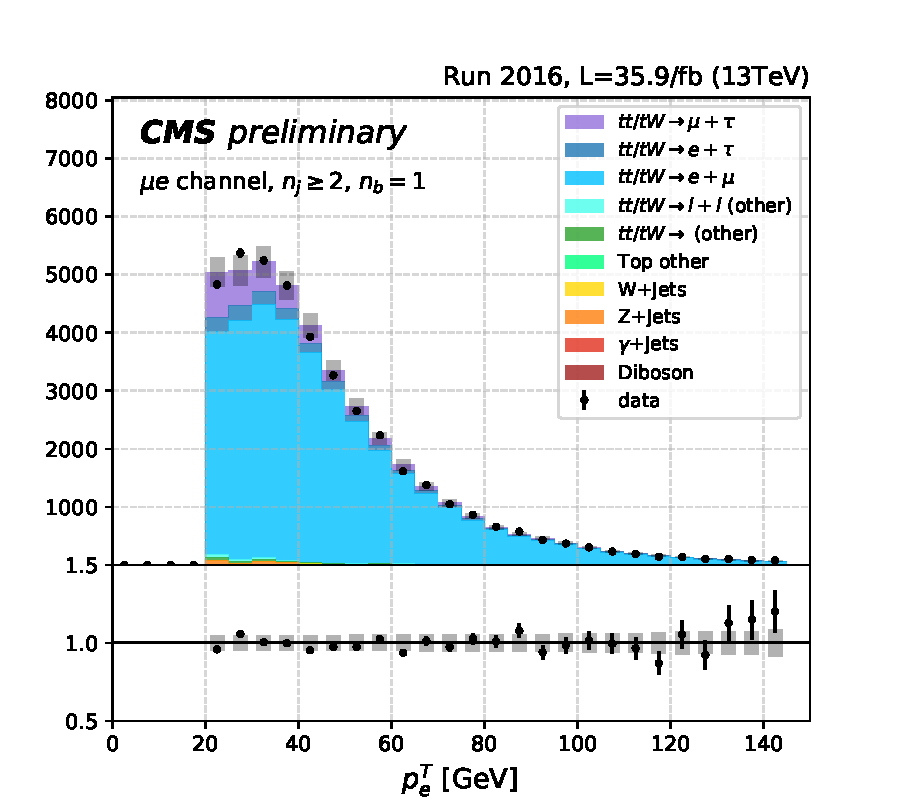
\includegraphics[width=0.24\textwidth]{chapters/Analysis/sectionPlots/figures/kinematics_pickles/emu/1b/emu_1b_lepton2_pt.pdf}
        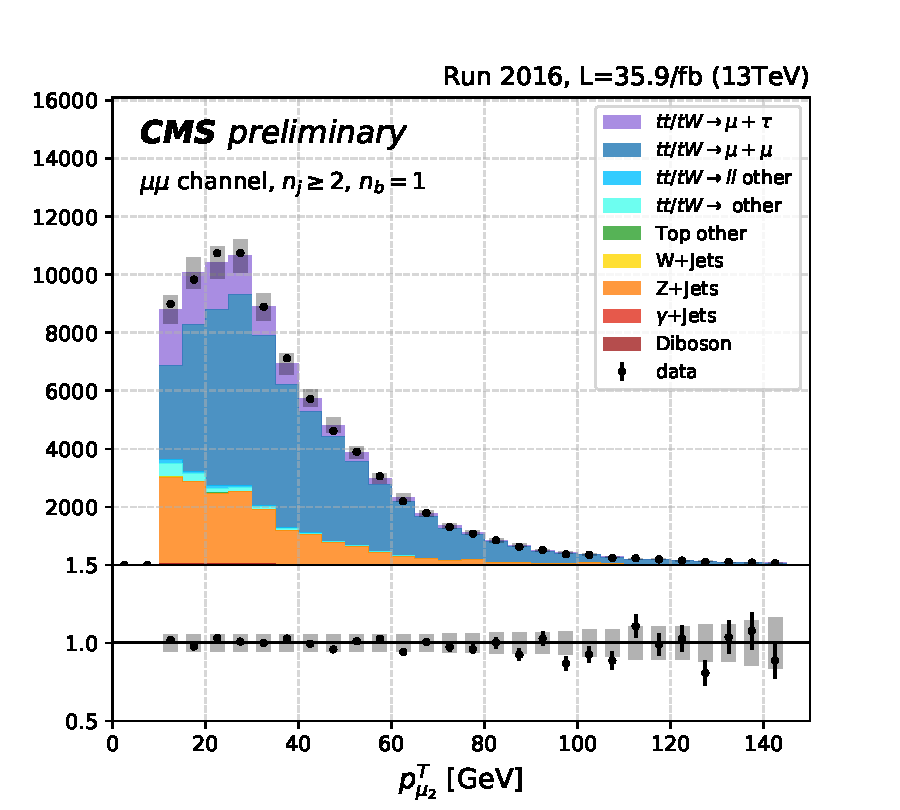
\includegraphics[width=0.24\textwidth]{chapters/Analysis/sectionPlots/figures/kinematics_pickles/mumu/1b/mumu_1b_lepton2_pt.pdf}
        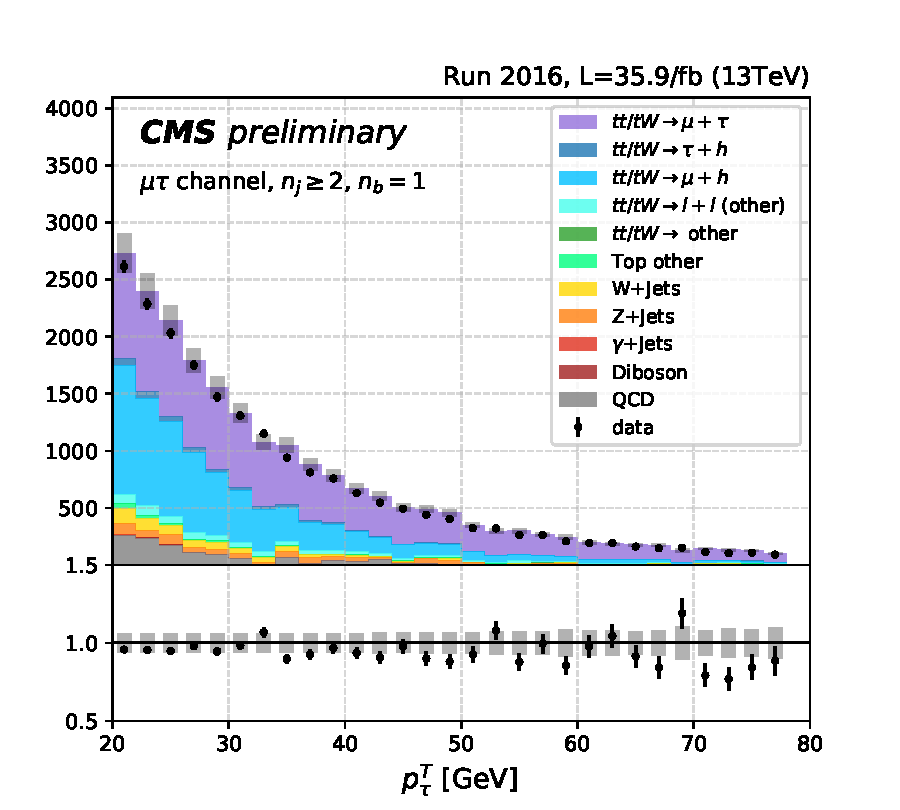
\includegraphics[width=0.24\textwidth]{chapters/Analysis/sectionPlots/figures/kinematics_pickles/mutau/1b/mutau_1b_lepton2_pt.pdf}
        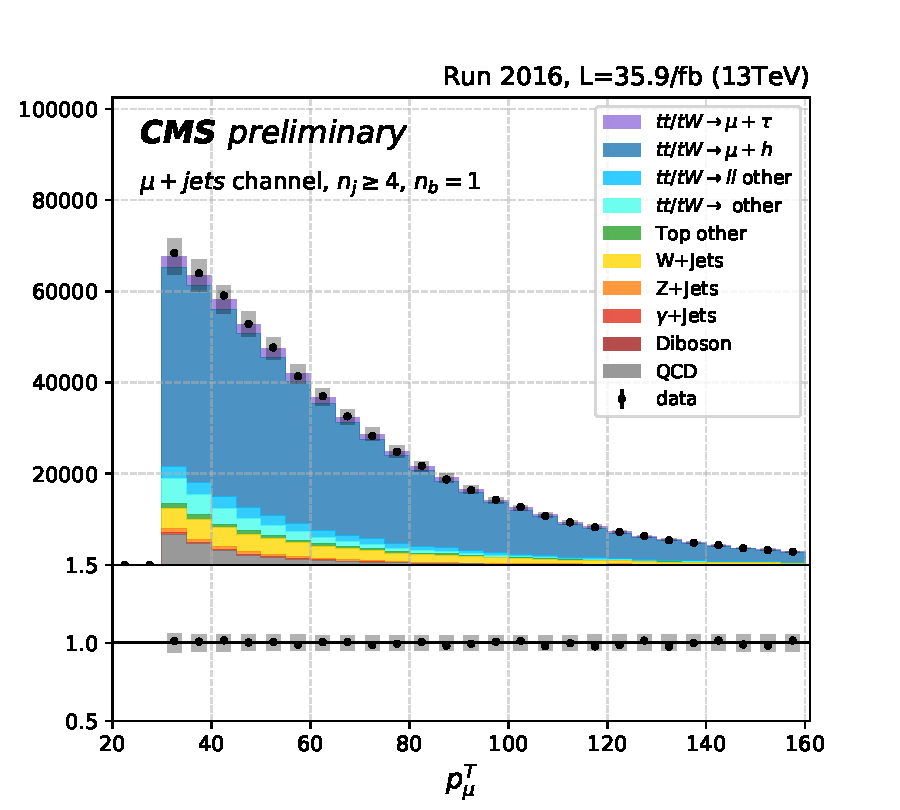
\includegraphics[width=0.24\textwidth]{chapters/Analysis/sectionPlots/figures/kinematics_pickles/mu4j/1b/mu4j_1b_lepton1_pt.pdf}
    \end{center}
    \end{block}
    
    \begin{block}{\smaller \Pe trigger}
    \begin{center}
        \cee \qquad\qquad\qquad\quad \cem \qquad\qquad\qquad\quad \cet \qquad\qquad\qquad\quad \ceh \\
        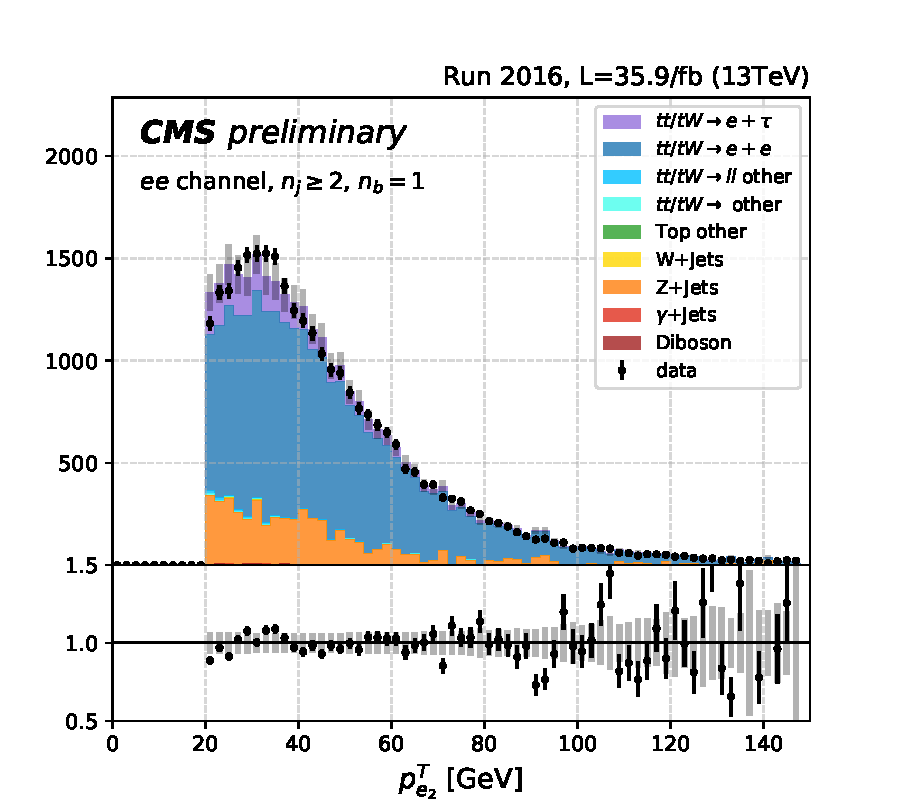
\includegraphics[width=0.24\textwidth]{chapters/Analysis/sectionPlots/figures/kinematics_pickles/ee/1b/ee_1b_lepton2_pt.pdf}
        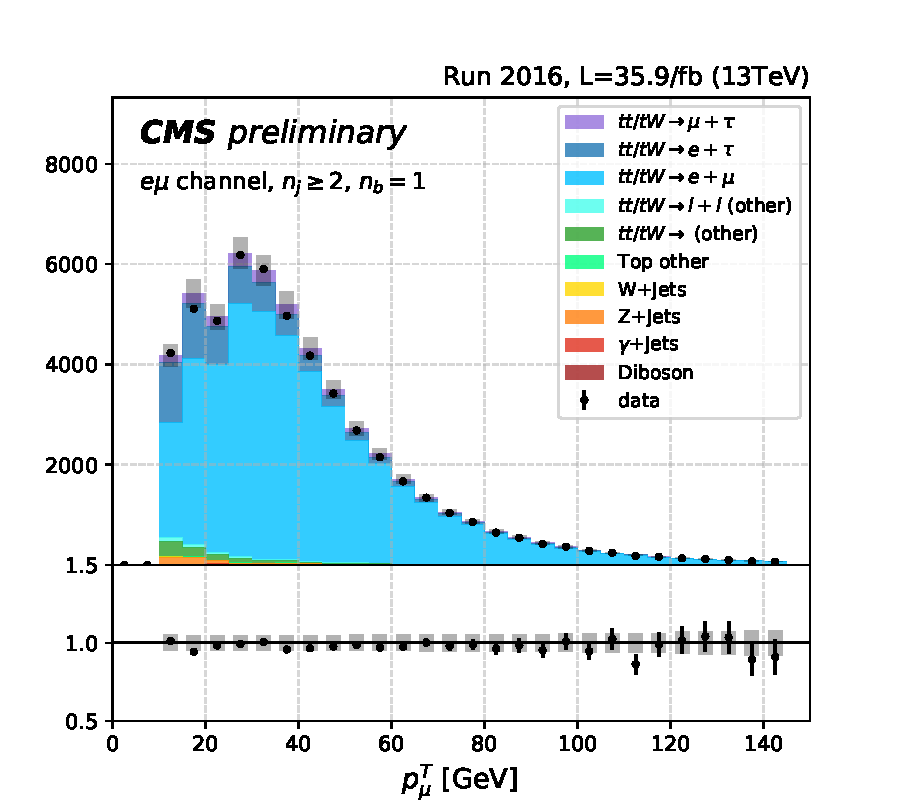
\includegraphics[width=0.24\textwidth]{chapters/Analysis/sectionPlots/figures/kinematics_pickles/emu2/1b/emu2_1b_lepton1_pt.pdf}
        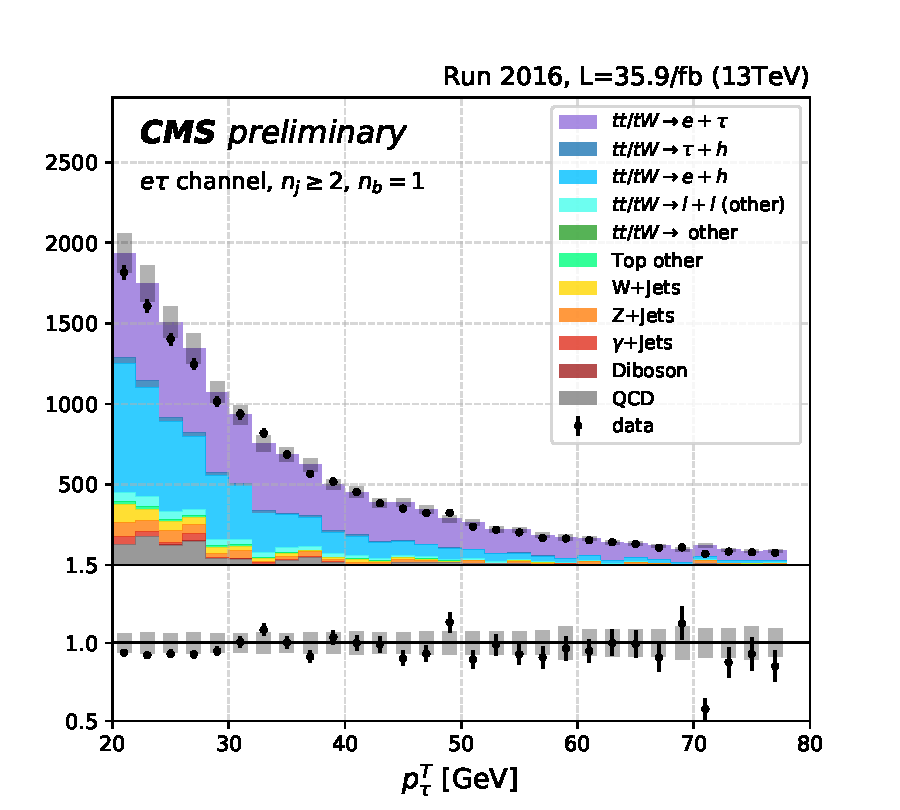
\includegraphics[width=0.24\textwidth]{chapters/Analysis/sectionPlots/figures/kinematics_pickles/etau/1b/etau_1b_lepton2_pt.pdf}
        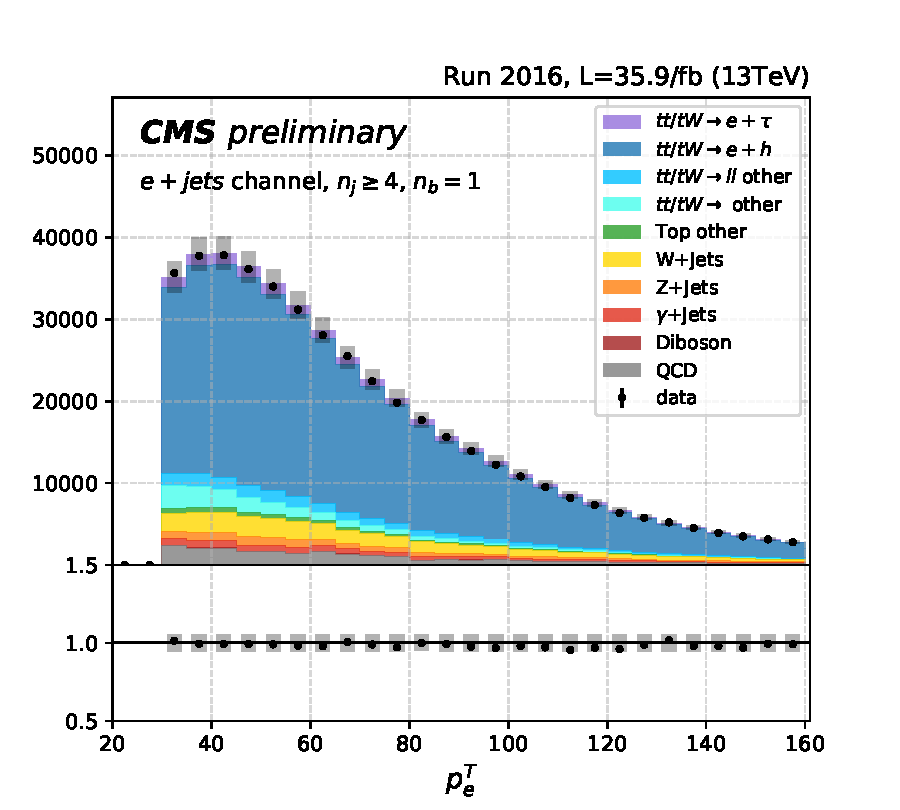
\includegraphics[width=0.24\textwidth]{chapters/Analysis/sectionPlots/figures/kinematics_pickles/e4j/1b/e4j_1b_lepton1_pt.pdf}
    \end{center}
    \end{block}
    
\end{frame}




\begin{frame}{}
    Baseline categories with $n_b\geq2$
    \begin{block}{\smaller \PGm trigger}
    \begin{center}
        \cme \qquad\qquad\qquad\quad \cmm \qquad\qquad\qquad\quad \cmt \qquad\qquad\qquad\quad \cmh \\
        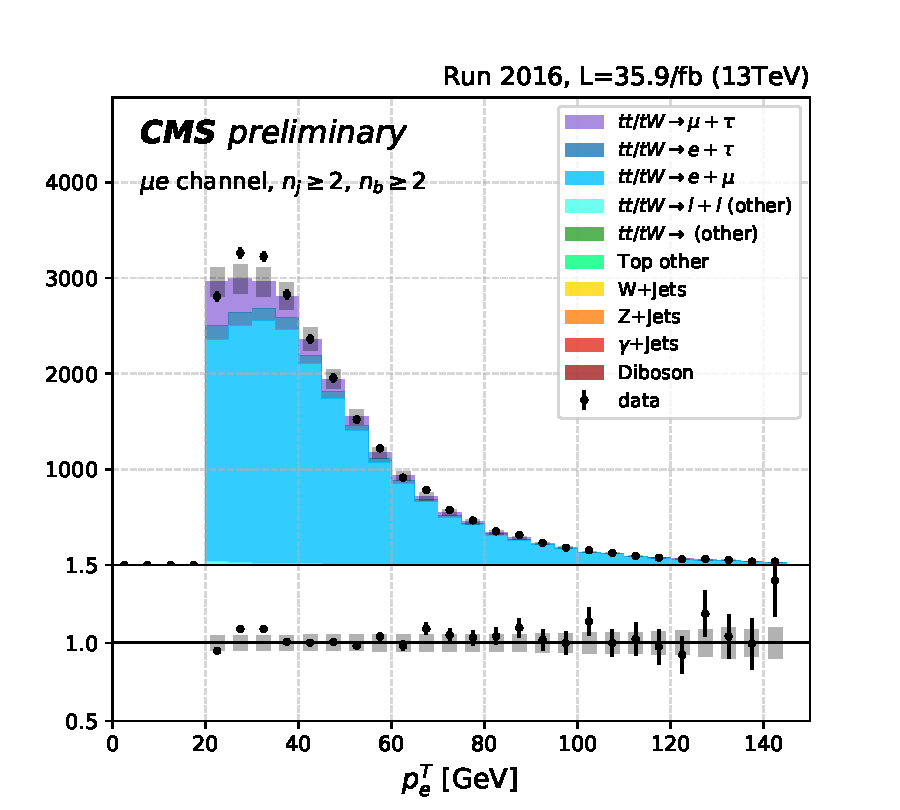
\includegraphics[width=0.24\textwidth]{chapters/Analysis/sectionPlots/figures/kinematics_pickles/emu/2b/emu_2b_lepton2_pt.pdf}
        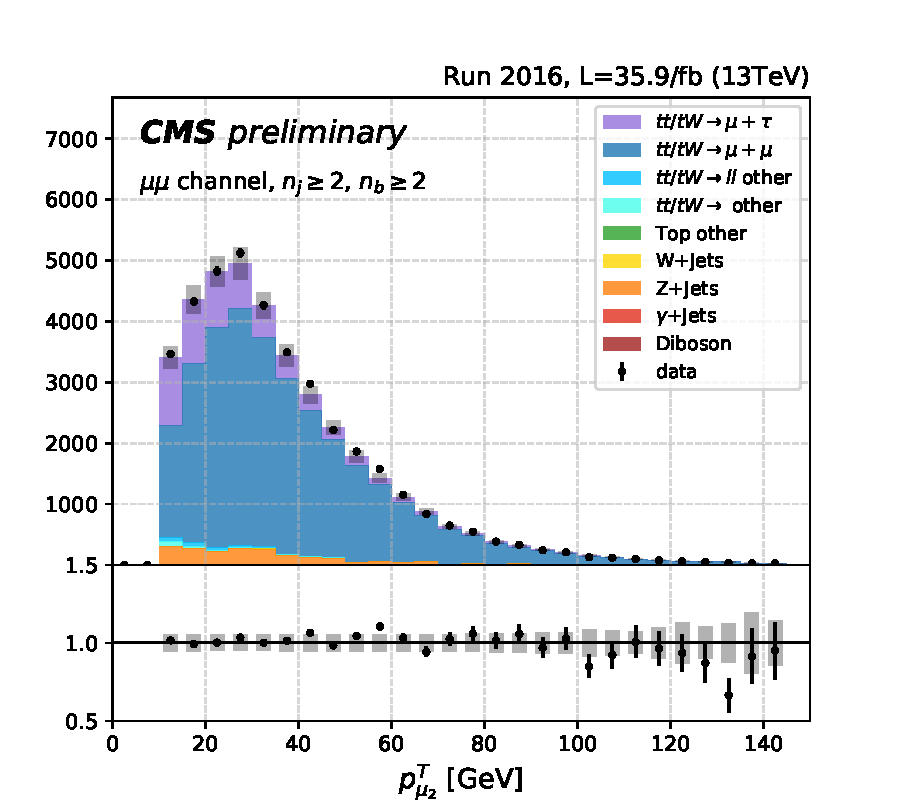
\includegraphics[width=0.24\textwidth]{chapters/Analysis/sectionPlots/figures/kinematics_pickles/mumu/2b/mumu_2b_lepton2_pt.pdf}
        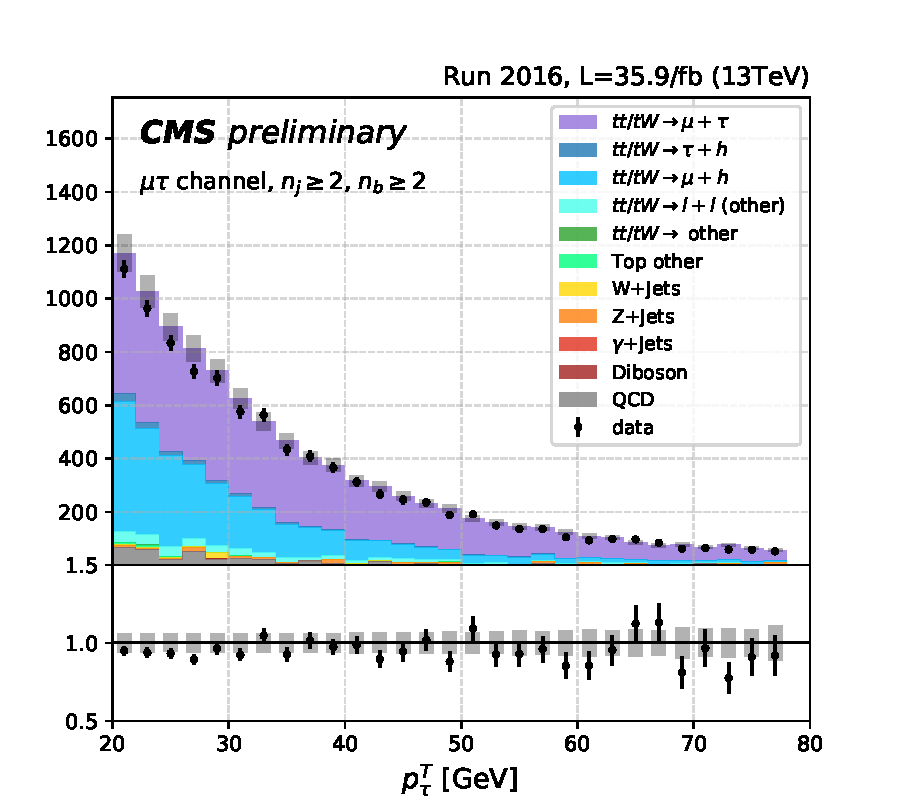
\includegraphics[width=0.24\textwidth]{chapters/Analysis/sectionPlots/figures/kinematics_pickles/mutau/2b/mutau_2b_lepton2_pt.pdf}
        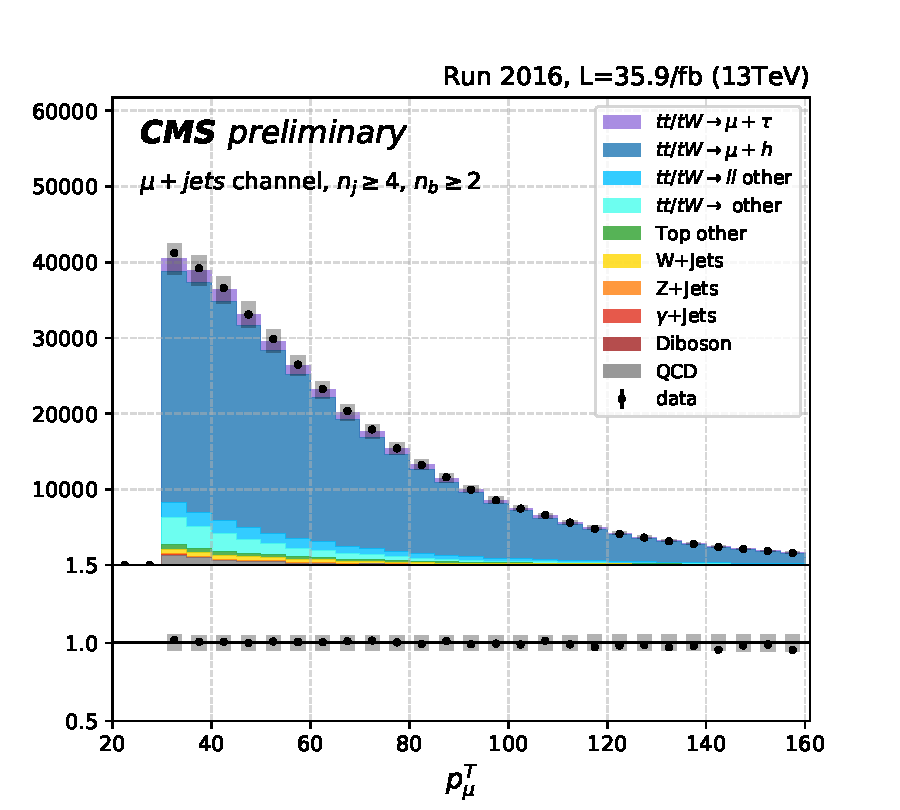
\includegraphics[width=0.24\textwidth]{chapters/Analysis/sectionPlots/figures/kinematics_pickles/mu4j/2b/mu4j_2b_lepton1_pt.pdf}
    \end{center}
    \end{block}
    
    \begin{block}{\smaller \Pe trigger}
    \begin{center}
        \cee \qquad\qquad\qquad\quad \cem \qquad\qquad\qquad\quad \cet \qquad\qquad\qquad\quad \ceh \\
        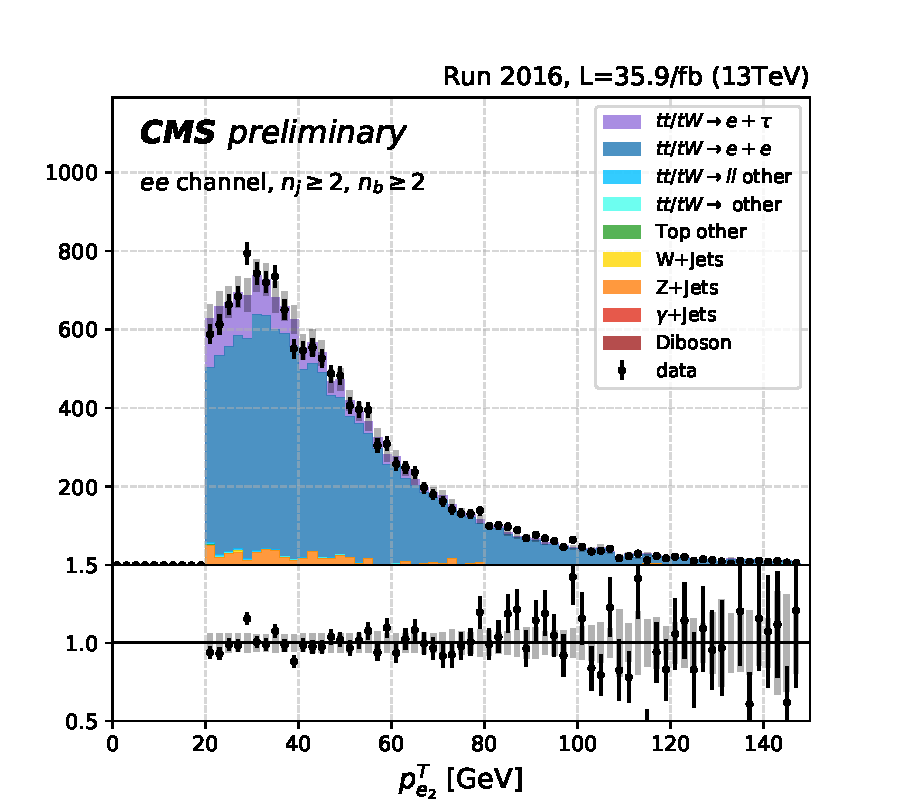
\includegraphics[width=0.24\textwidth]{chapters/Analysis/sectionPlots/figures/kinematics_pickles/ee/2b/ee_2b_lepton2_pt.pdf}
        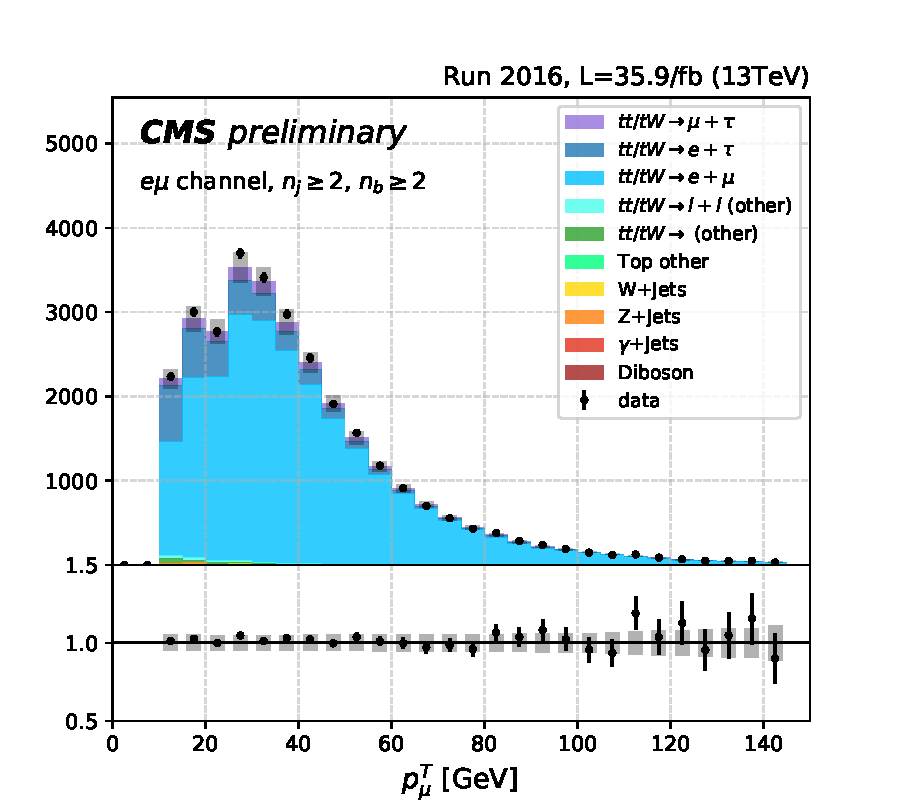
\includegraphics[width=0.24\textwidth]{chapters/Analysis/sectionPlots/figures/kinematics_pickles/emu2/2b/emu2_2b_lepton1_pt.pdf}
        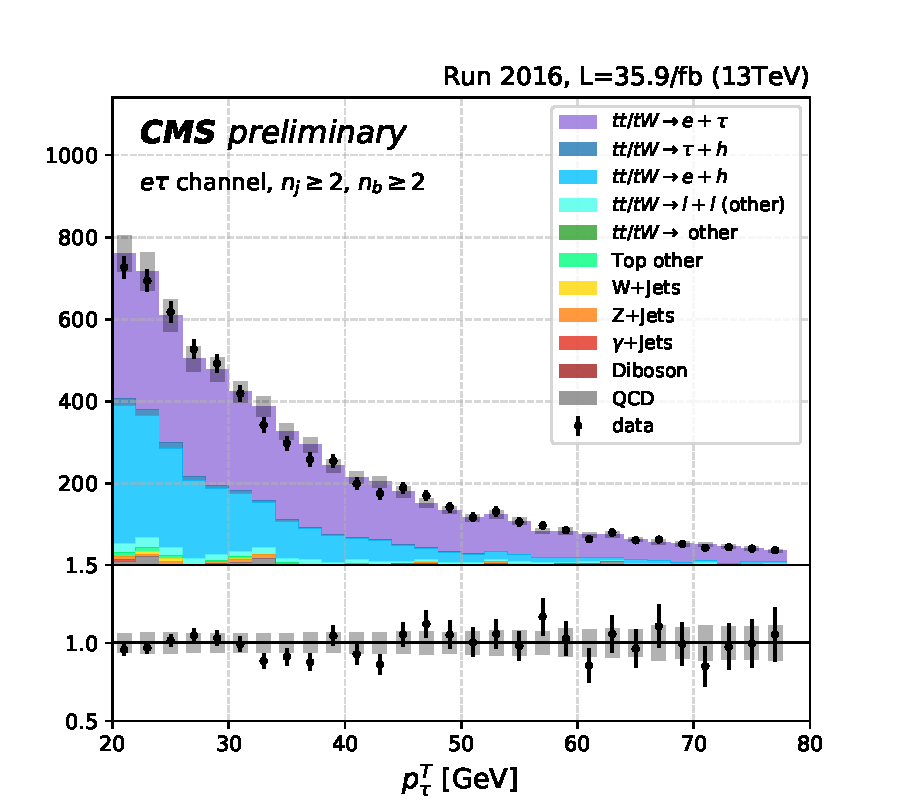
\includegraphics[width=0.24\textwidth]{chapters/Analysis/sectionPlots/figures/kinematics_pickles/etau/2b/etau_2b_lepton2_pt.pdf}
        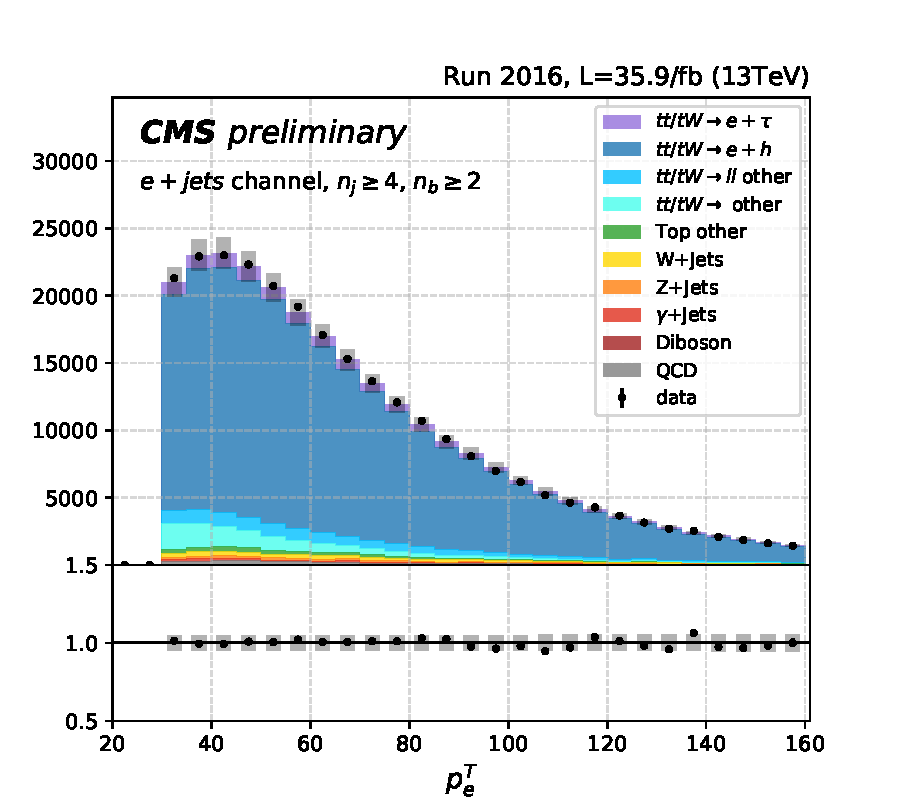
\includegraphics[width=0.24\textwidth]{chapters/Analysis/sectionPlots/figures/kinematics_pickles/e4j/2b/e4j_2b_lepton1_pt.pdf}
    \end{center}
    \end{block}
\end{frame}





% -------------
% new frame
% -------------
\begin{frame}{Extended $n_j$ and $n_b$ categories}
\smaller
    \begin{table}
        \centering
        \setlength{\tabcolsep}{1em}
        \renewcommand{\arraystretch}{1.5}
        \resizebox{0.7\textwidth}{!}{\begin{tabular}{l|c|c|c c|c}

                                    & $N_j = 0$     & $N_j = 1$      & $N_j = 2$                    & \multicolumn{1}{|c|}{$N_j = 3$}   & $N_j \geq 4$ \\
	\hline
    \multirow{2}{*}{$N_\PQb = 0$}   & \cellcolor{NUpurple10}\textcolor{red}{\cet, \cmt,}  & \cellcolor{NUpurple10}\textcolor{red}{\cet, \cmt,} & \multicolumn{2}{c}{\cellcolor{NUpurple10} \textcolor{red}{\cet, \cmt,} }      & \cellcolor{NUpurple10}\\
                                    & \cellcolor{NUpurple10} \textcolor{blue}{\cem}         & \cellcolor{NUpurple10}\textcolor{blue}{\cem}       & \multicolumn{2}{c}{\cellcolor{NUpurple10} \textcolor{orange}{\cem}}& \cellcolor{NUpurple10}\\
	\hline
    \multirow{3}{*}{$N_\PQb = 1$}   &   & \cellcolor{NUpurple10} \textcolor{orange}{\cet, \cmt, \cem } & \cet, \cmt   & \multicolumn{2}{!{\color{OliveGreen}\vrule width 2pt}c}{\cet, \cmt} \\
	\cline{3-6}
                                    & \multicolumn{2}{c|}{} & \multicolumn{3}{c}{ \cee, \cmm, \cem}                                        \\
	\cline{4-6}
                                    & \multicolumn{4}{c|}{} & \ceh, \cmh \\
	\hline

    \multirow{3}{*}{$N_\PQb \geq 2$} & \multicolumn{2}{c|}{} & \cet, \cmt & \multicolumn{2}{!{\color{OliveGreen}\vrule width 2pt}c}{\cet, \cmt} \\
	\cline{4-6}
                                    & \multicolumn{2}{c|}{} & \multicolumn{3}{c}{$\cee, \cmm, \cem$}                                        \\
	\cline{4-6}
                                    & \multicolumn{4}{c|}{} & \ceh, \cmh \\
	\hline
\end{tabular}}
    \end{table}

    \begin{block}{extended $n_j$ and $n_b$ categories in shape analysis}
    \begin{itemize}
        \item \textcolor{red}{Enriched with $\PZ \to \PGtl \PGth$ to constrain \PGth systematics.}
        extra cuts on $m_{\ell \PGth}$, $\Delta\phi(\ell,\PGth)$, $\mT^{\ell,MET}$ to enhance \zjets over \wjets.
        \item \textcolor{OliveGreen}{Bin $n_j$ finer in \cet and \cmt to better discriminate $\PW\to \PGth$ and $\PW\to jj$}
        \item \textcolor{blue}{Add \WW events}
        \item \textcolor{orange}{Add more \ttbar events}
    \end{itemize}
    \end{block}
\end{frame}


% -------------
% new frame
% -------------
\begin{frame}{}

    \begin{tcolorbox}[colframe=red,colback=white]{$\PZ\to \PGtl \PGth$}
    \smaller
        \begin{center}
        \color{red}
        $\cet: n_j=0, n_b=0$ \hspace{0.12\textwidth} $n_j=1, n_b=0$ \hspace{0.12\textwidth} $n_j\geq2, n_b=0$ \\
        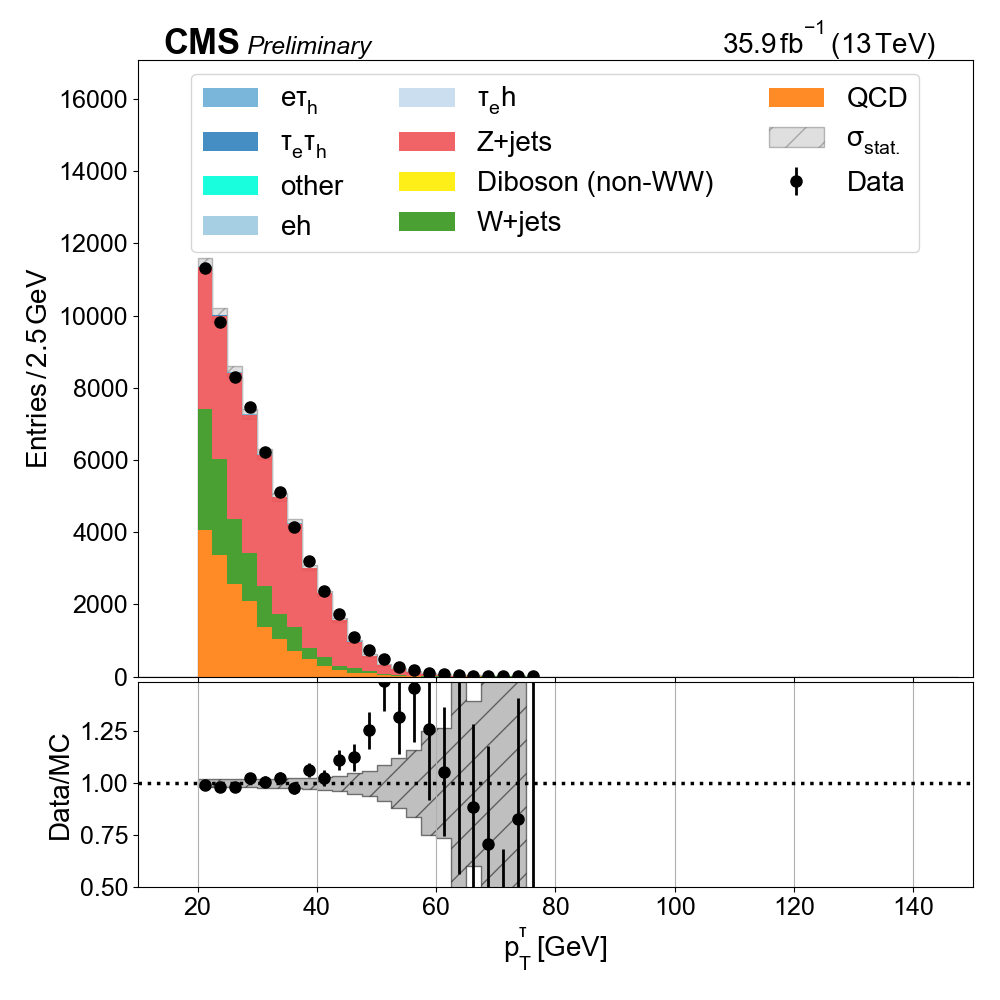
\includegraphics[width=0.3\textwidth]{chapters/Analysis/sectionPlots/figures/data_mc_overlays/etau_2016_cat_eq0_eq0_signal_linear_lepton_lepton2_pt.png}
        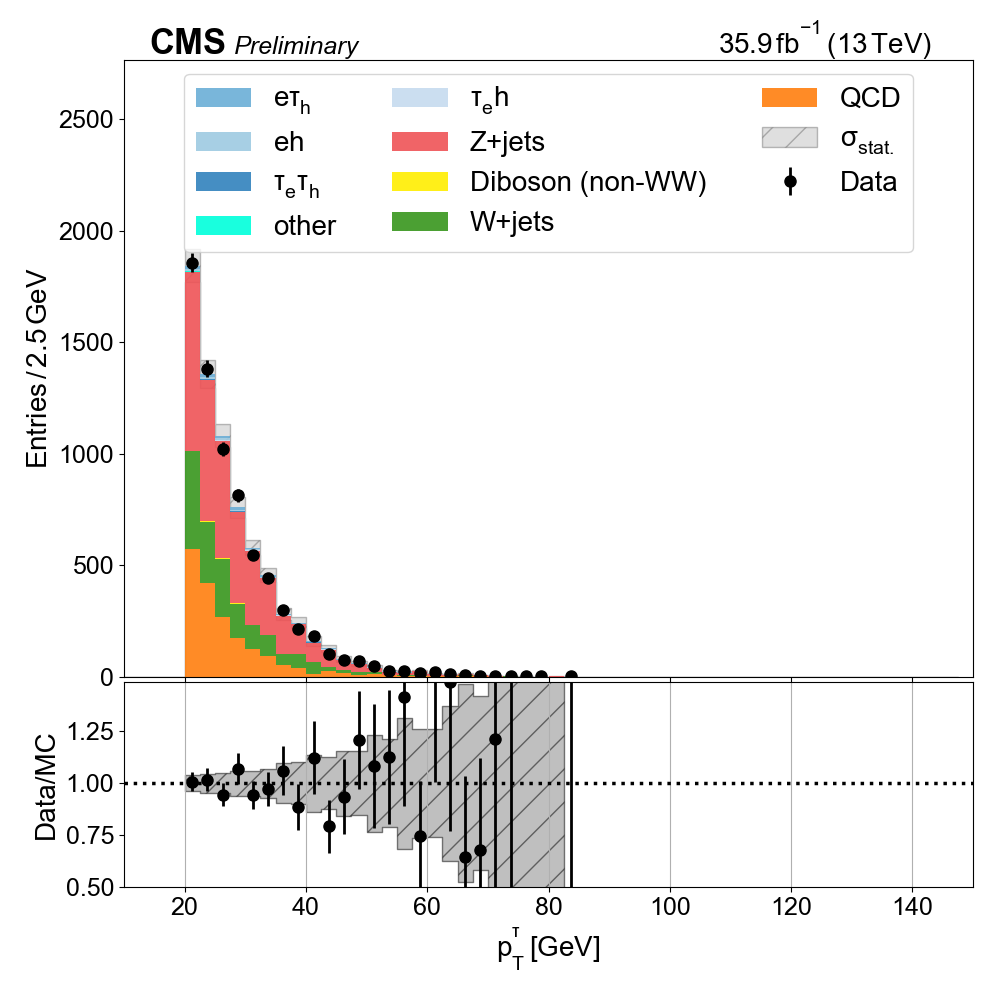
\includegraphics[width=0.3\textwidth]{chapters/Analysis/sectionPlots/figures/data_mc_overlays/etau_2016_cat_eq1_eq0_signal_linear_lepton_lepton2_pt.png}
        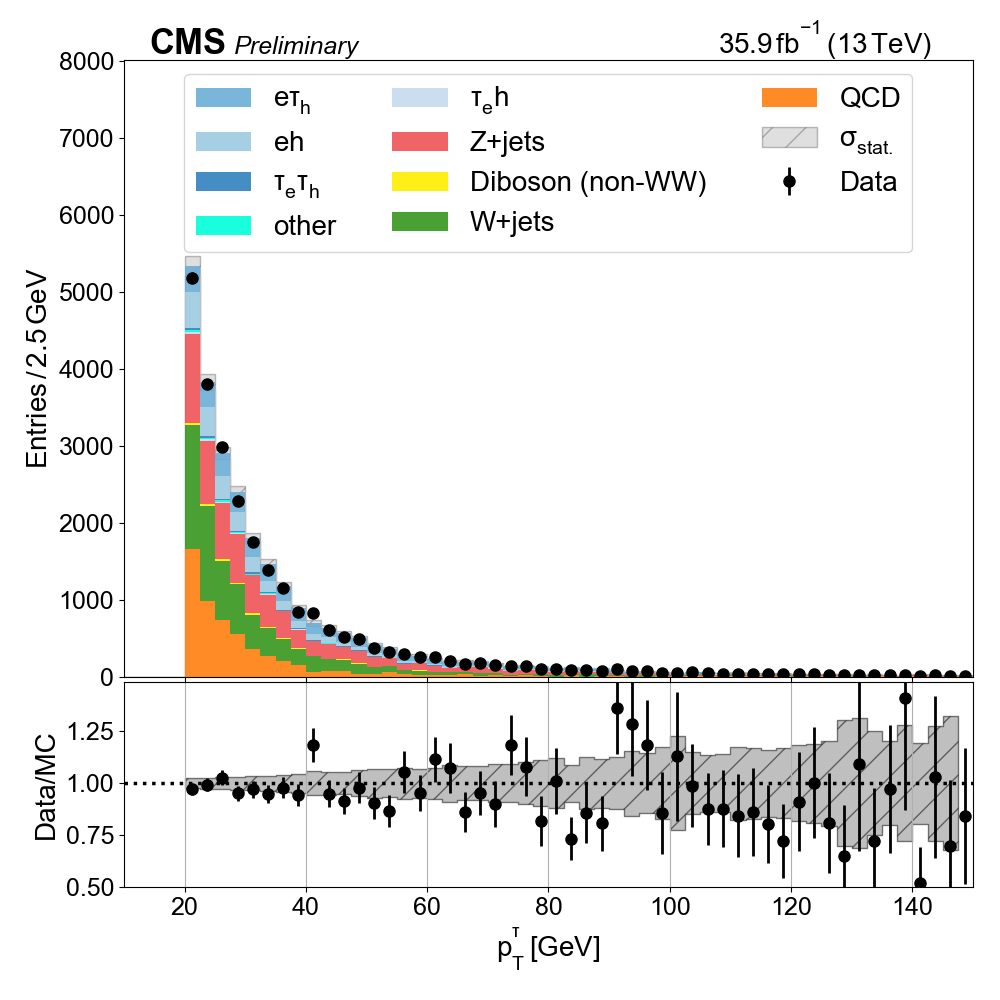
\includegraphics[width=0.3\textwidth]{chapters/Analysis/sectionPlots/figures/data_mc_overlays/etau_2016_cat_gt2_eq0_signal_linear_lepton_lepton2_pt.png} \\
        $\cmt: n_j=0, n_b=0$ \hspace{0.12\textwidth} $n_j=1, n_b=0$ \hspace{0.12\textwidth} $n_j\geq2, n_b=0$ \\
        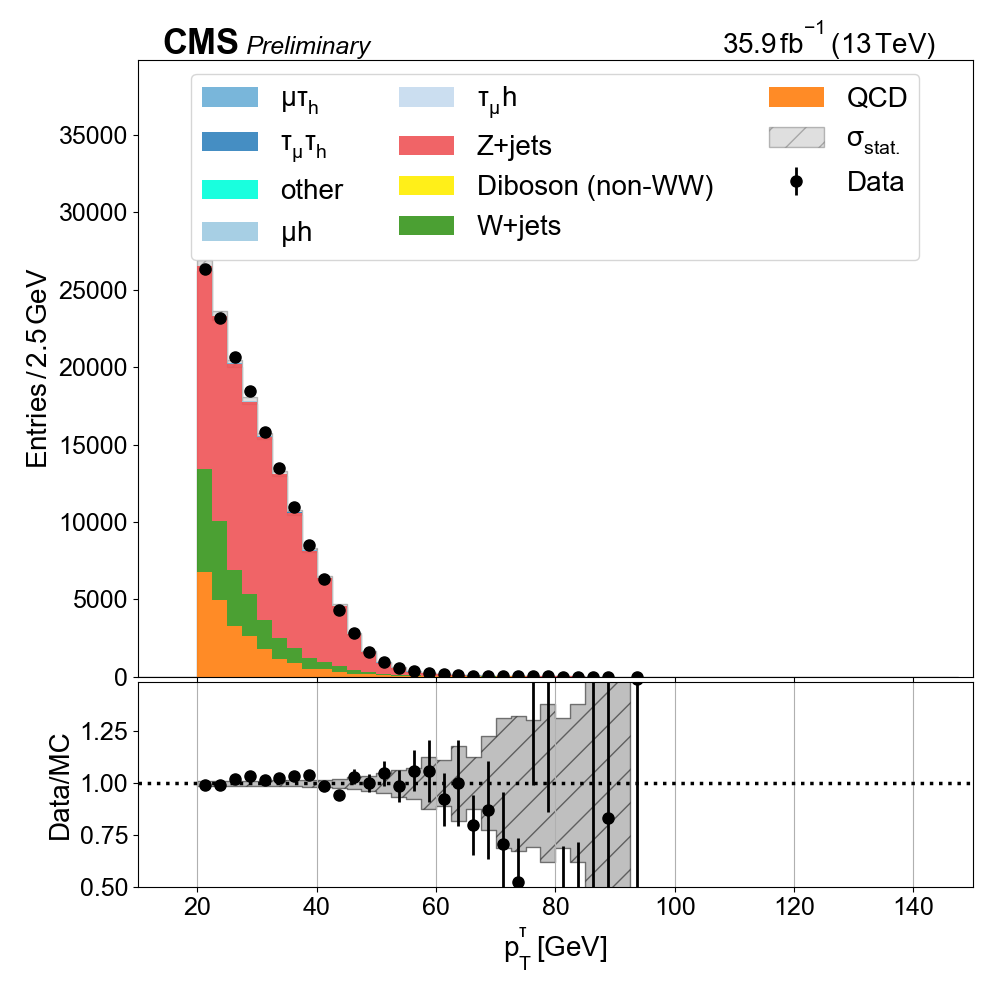
\includegraphics[width=0.3\textwidth]{chapters/Analysis/sectionPlots/figures/data_mc_overlays/mutau_2016_cat_eq0_eq0_signal_linear_lepton_lepton2_pt.png}
        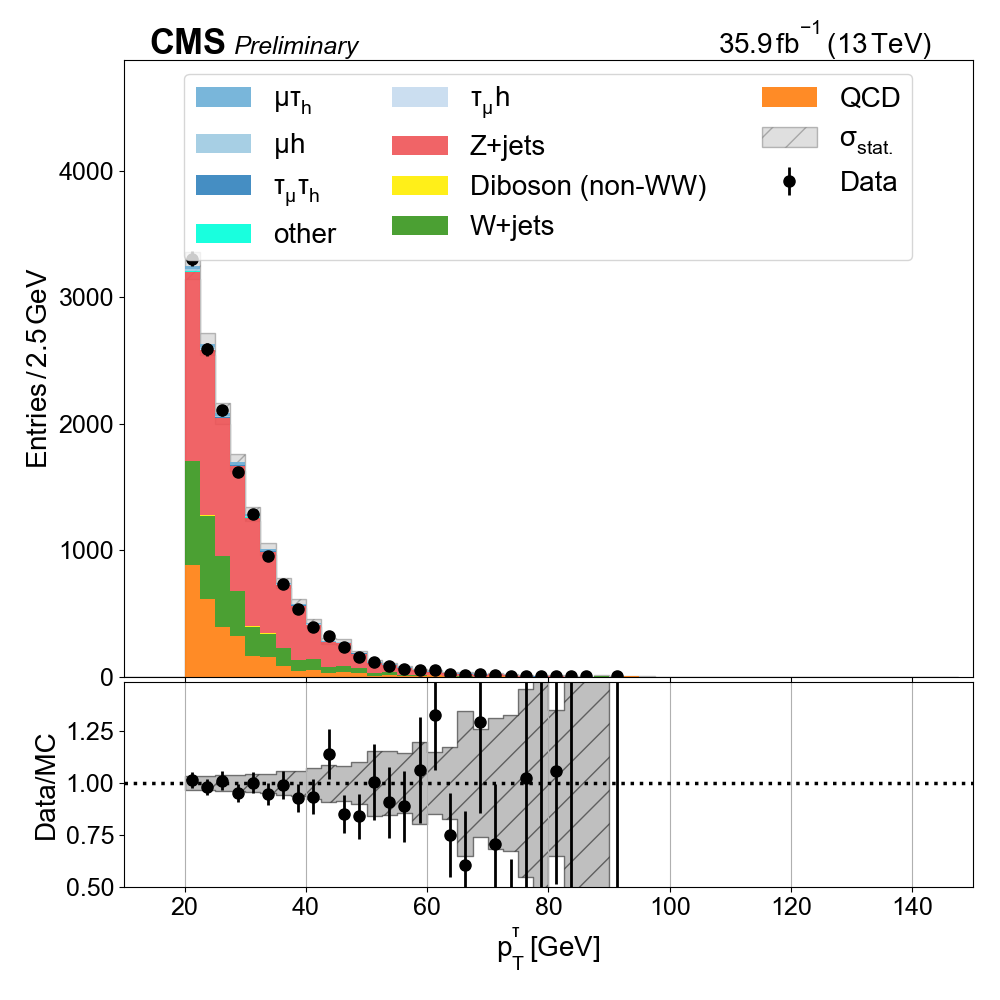
\includegraphics[width=0.3\textwidth]{chapters/Analysis/sectionPlots/figures/data_mc_overlays/mutau_2016_cat_eq1_eq0_signal_linear_lepton_lepton2_pt.png}
        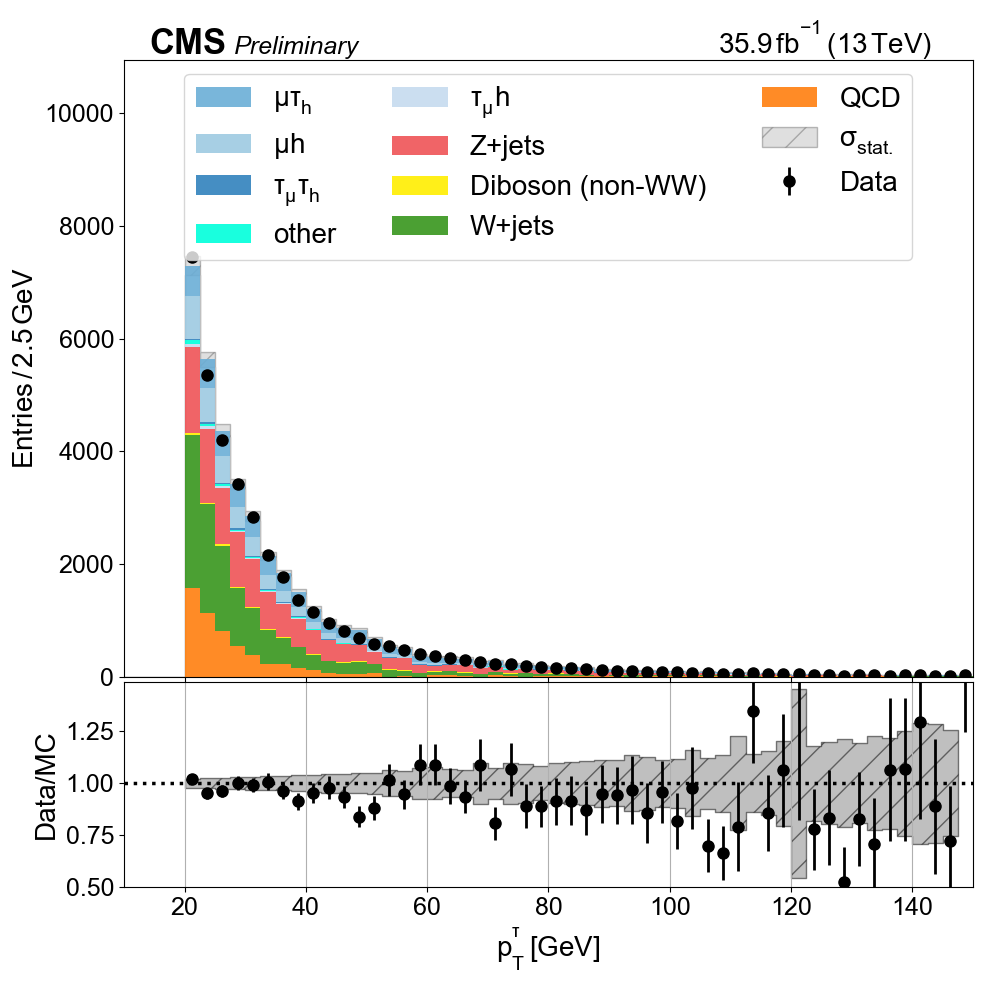
\includegraphics[width=0.3\textwidth]{chapters/Analysis/sectionPlots/figures/data_mc_overlays/mutau_2016_cat_gt2_eq0_signal_linear_lepton_lepton2_pt.png}        
        \end{center}
    \end{tcolorbox}
\end{frame}

% -------------
% new frame
% -------------
\begin{frame}{}
    \begin{columns}
        \column{0.33\textwidth}
        \begin{tcolorbox}[colframe=OliveGreen,colback=white]{finer $n_j$ binning}
            \begin{center}
            \color{OliveGreen}
            \smaller \smaller
            $n_j$ distribution of \cet\\
            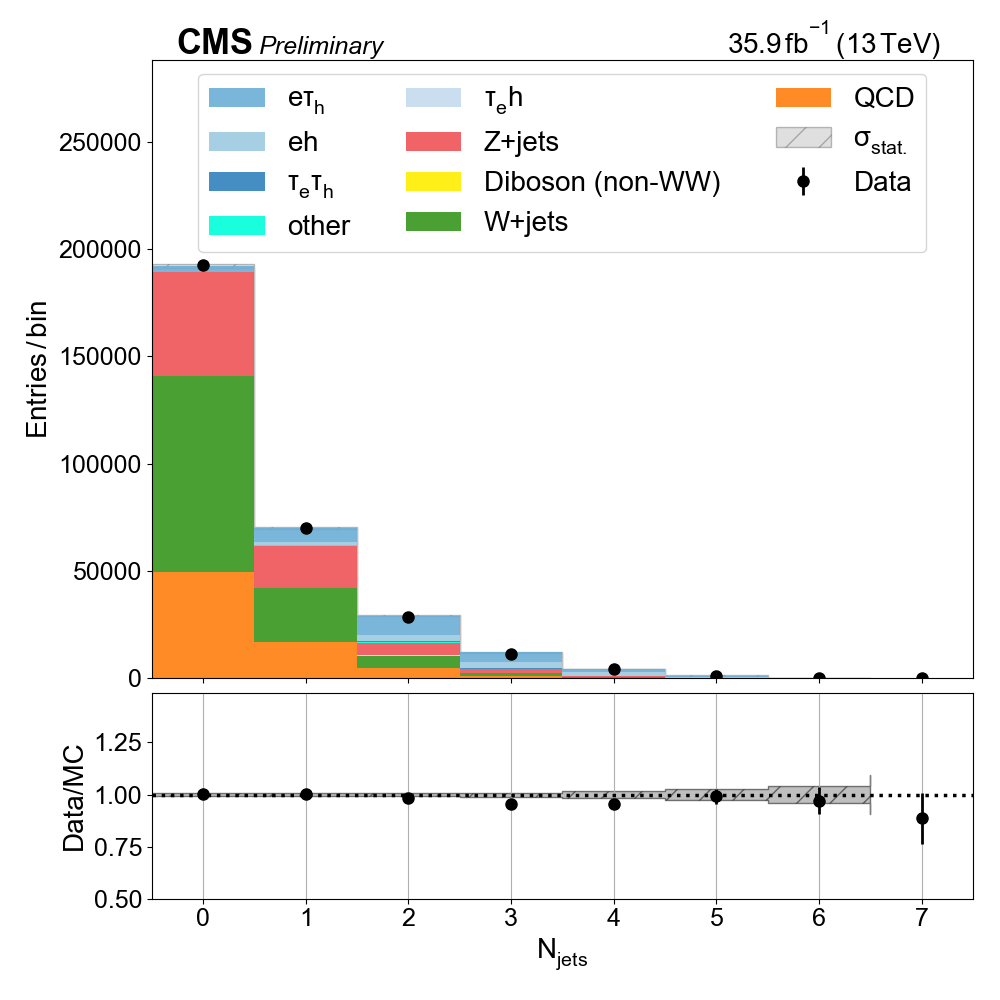
\includegraphics[width=\textwidth]{chapters/Analysis/sectionPlots/figures/data_mc_overlays/etau_2016_inclusive_linear_jet_n_jets.png}
            \end{center}
        \end{tcolorbox}
        
        \column{0.6\textwidth}
        \begin{tcolorbox}[colframe=blue,colback=white]{$\WW \to \Pe \PGm$}
            \begin{center}
            \color{blue}
            \smaller \smaller
            $\cem: n_j=0, n_b=0$ \hspace{0.1\textwidth} $n_j=1, n_b=0$  \\
            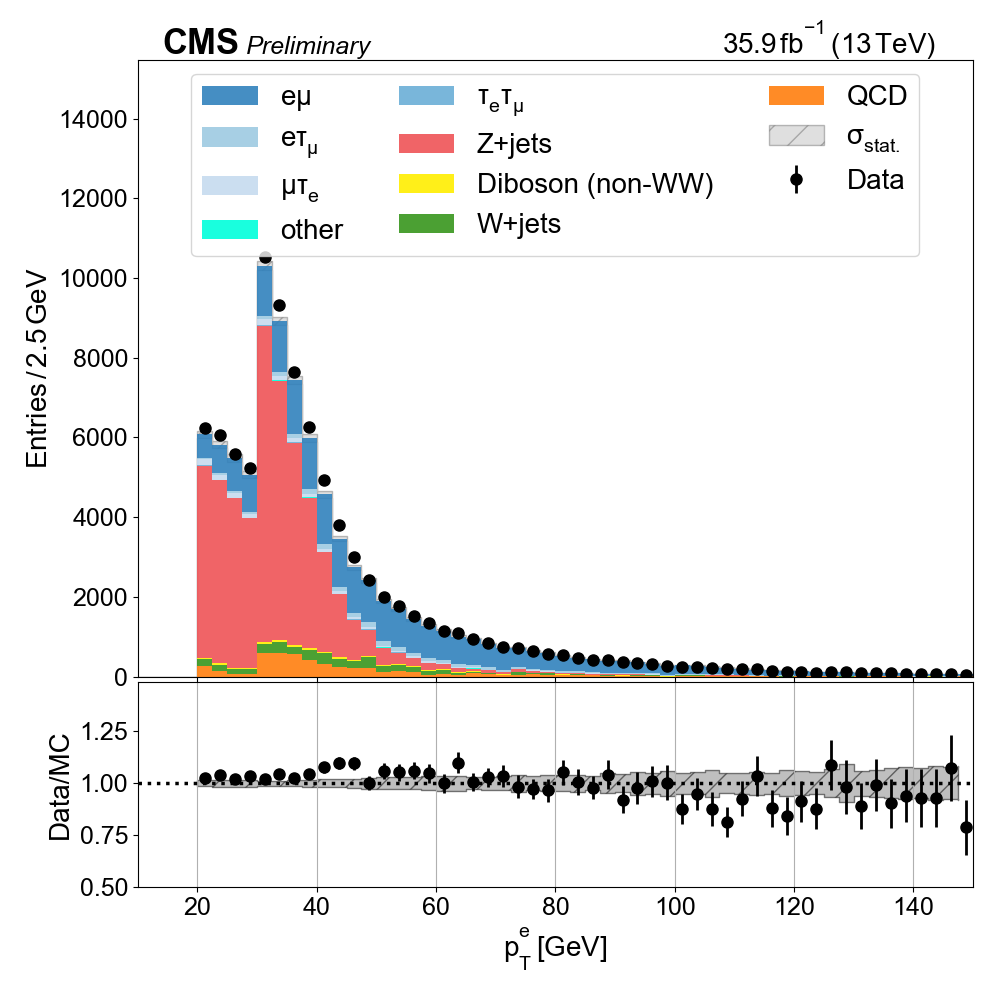
\includegraphics[width=0.48\textwidth]{chapters/Analysis/sectionPlots/figures/data_mc_overlays/emu_2016_cat_eq0_eq0_a_signal_linear_lepton_lepton2_pt.png}
            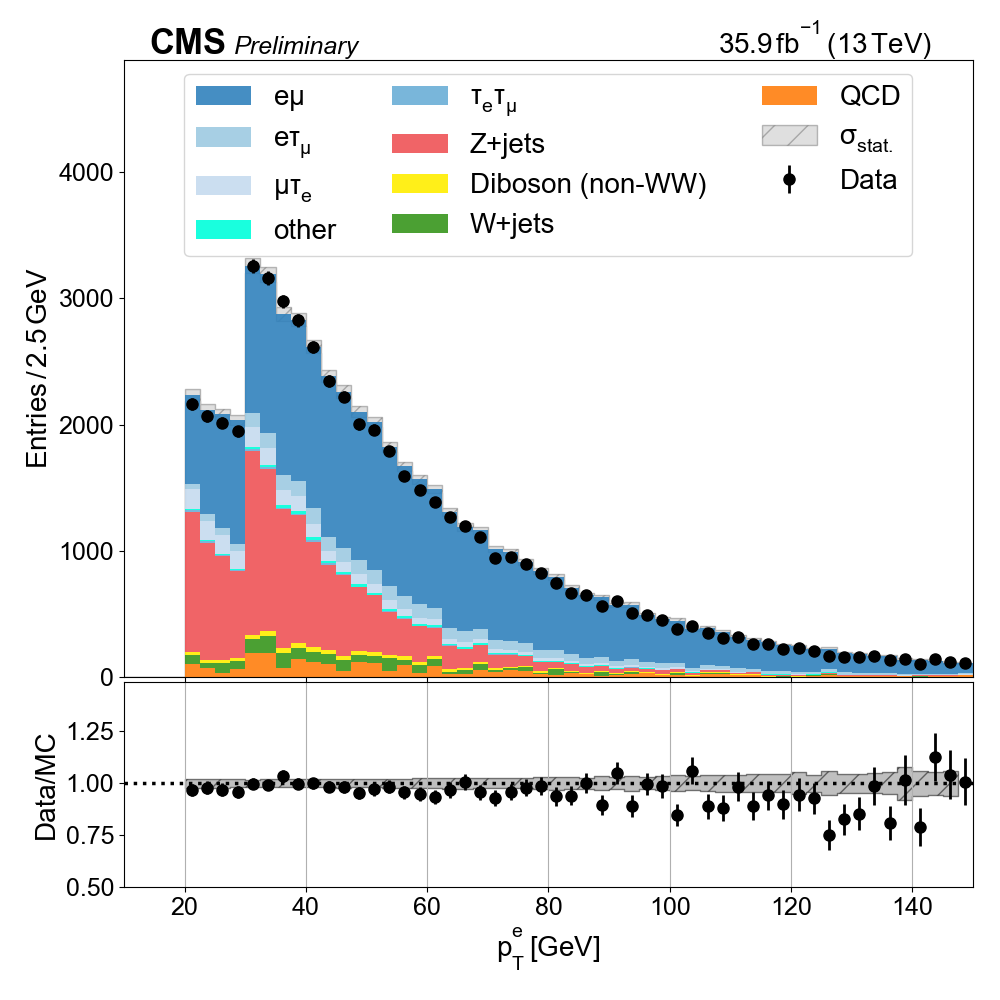
\includegraphics[width=0.48\textwidth]{chapters/Analysis/sectionPlots/figures/data_mc_overlays/emu_2016_cat_eq1_eq0_a_signal_linear_lepton_lepton2_pt.png}
            \end{center}
        \end{tcolorbox}
    \end{columns}
    
    
    \begin{tcolorbox}[colframe=orange,colback=white]{$\ttbar$ extra}
        \begin{center}
        \color{orange}
        \smaller \smaller
        $\cet: n_j=1, n_b=1$ \hspace{0.04\textwidth} $\cmt: n_j=1, n_b=1$ \hspace{0.04\textwidth} $\cem: n_j=1, n_b=1$ \hspace{0.04\textwidth} $\cem: n_j\geq2, n_b=0$ \\
        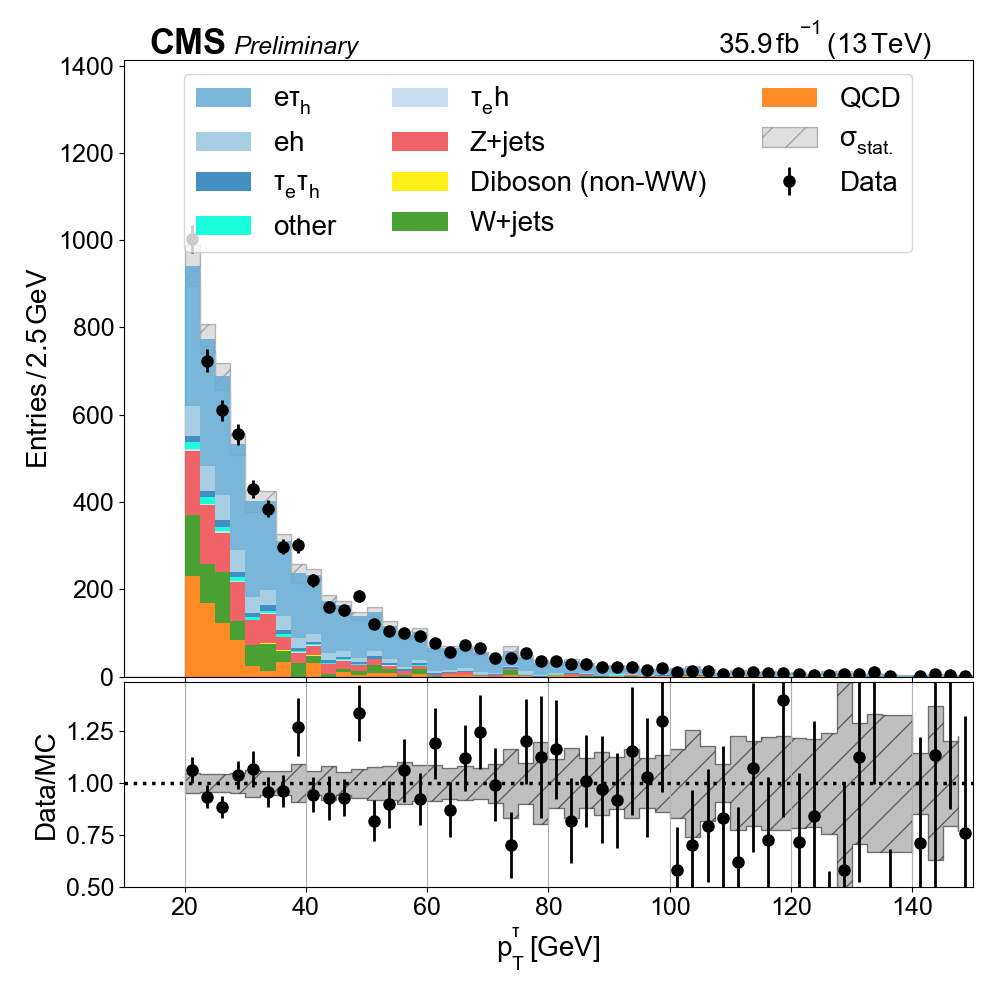
\includegraphics[width=0.24\textwidth]{chapters/Analysis/sectionPlots/figures/data_mc_overlays/etau_2016_cat_eq1_eq1_signal_linear_lepton_lepton2_pt.png}
        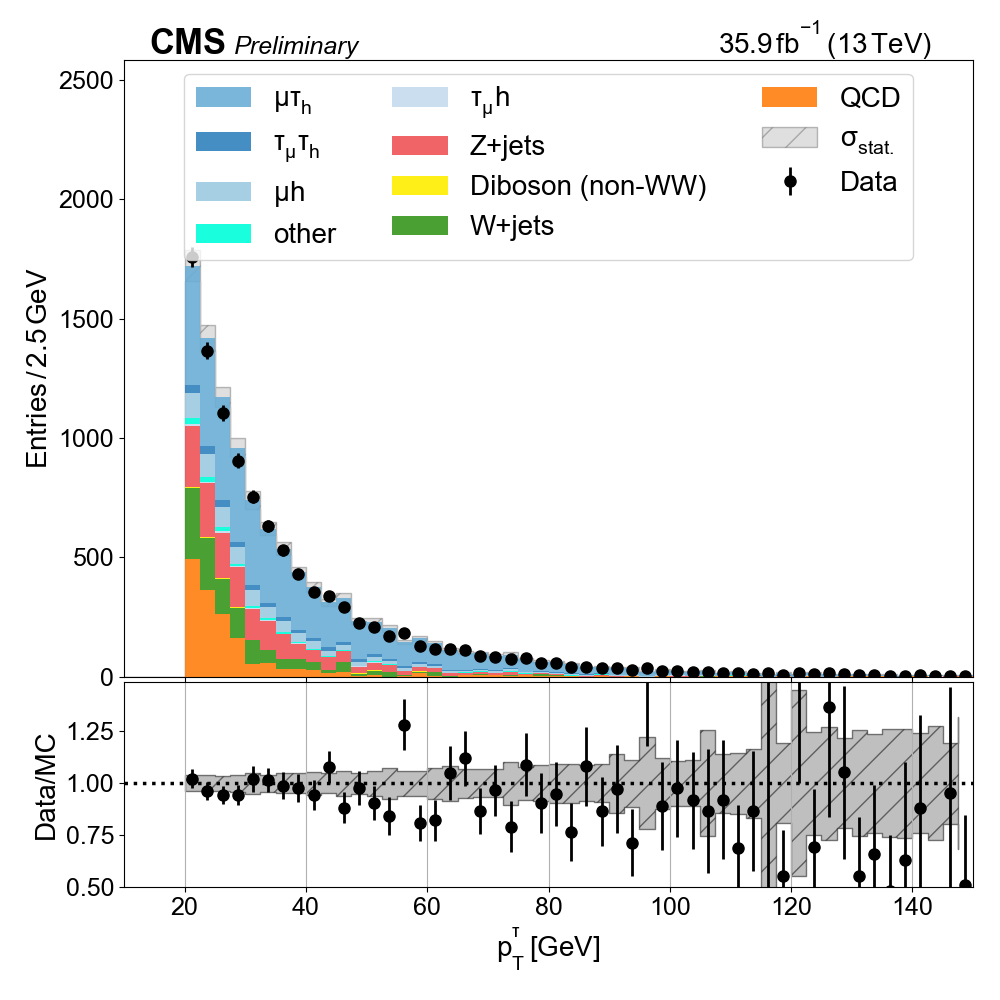
\includegraphics[width=0.24\textwidth]{chapters/Analysis/sectionPlots/figures/data_mc_overlays/mutau_2016_cat_eq1_eq1_signal_linear_lepton_lepton2_pt.png}
        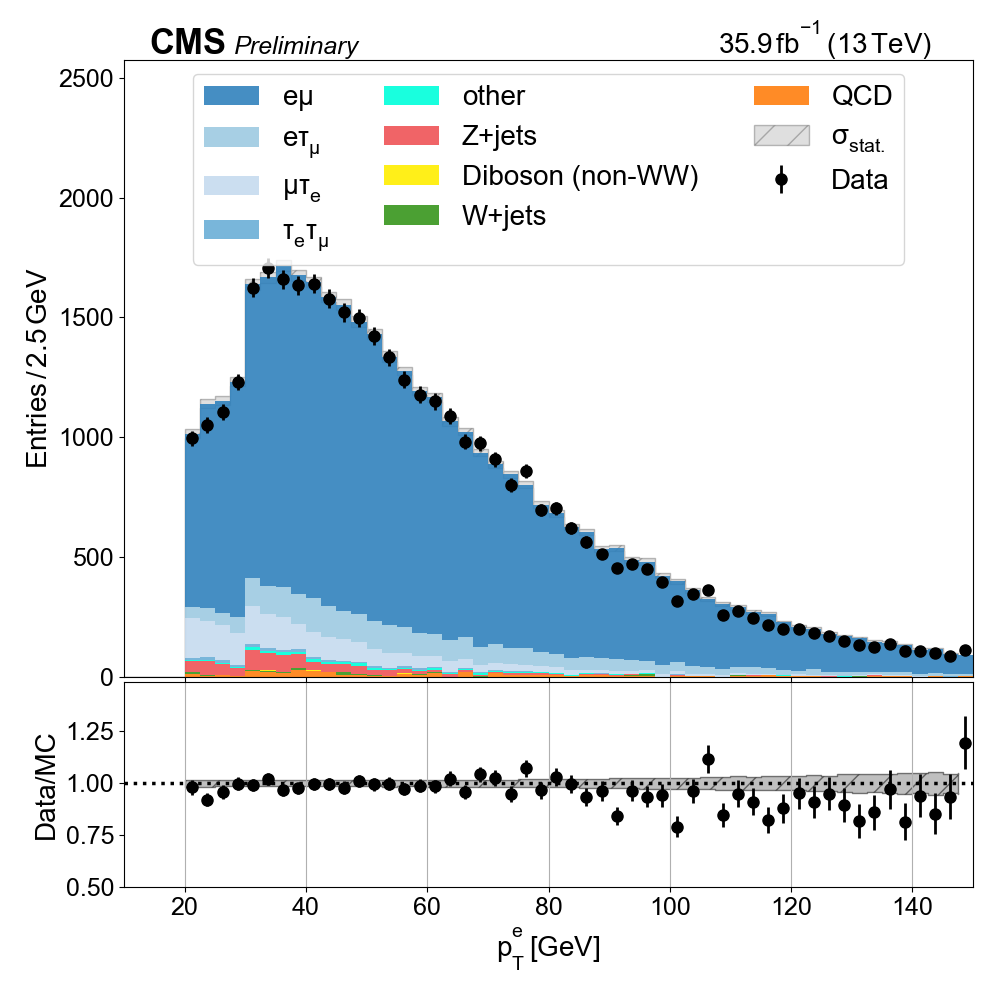
\includegraphics[width=0.24\textwidth]{chapters/Analysis/sectionPlots/figures/data_mc_overlays/emu_2016_cat_eq1_eq1_a_signal_linear_lepton_lepton2_pt.png}
        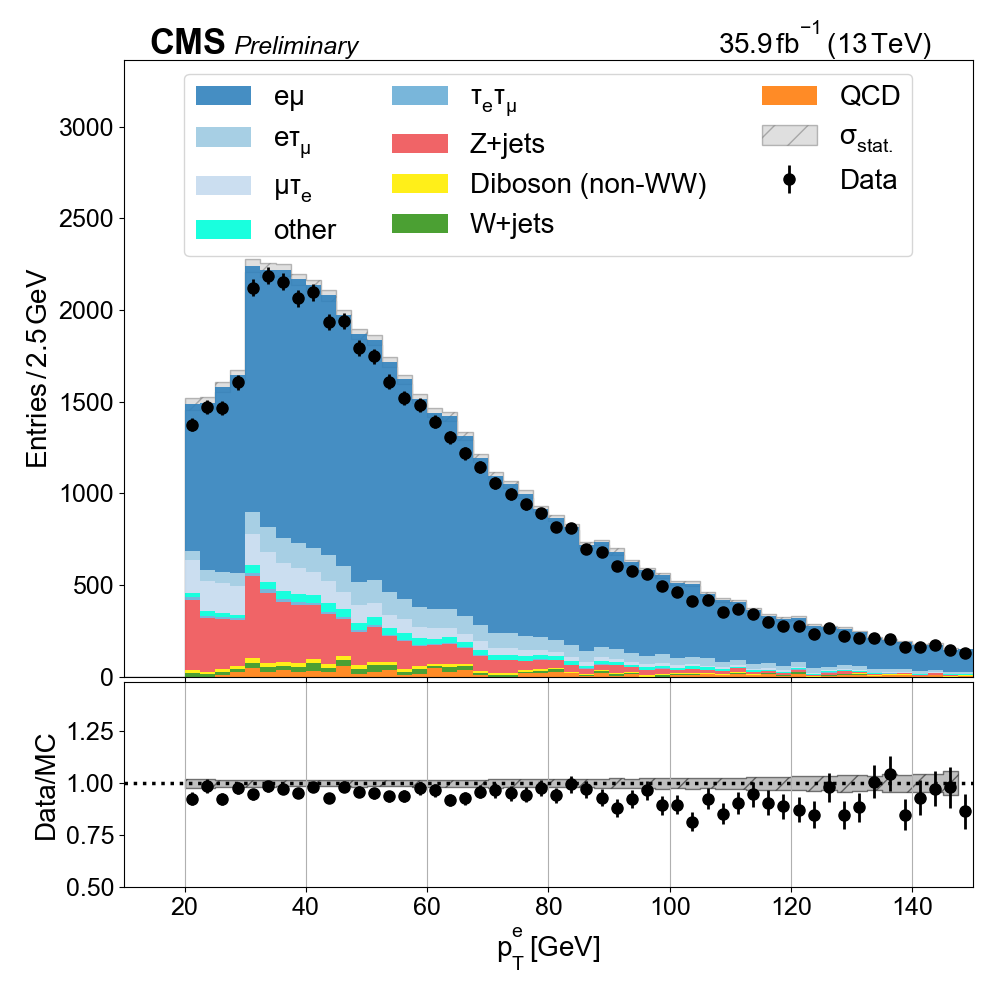
\includegraphics[width=0.24\textwidth]{chapters/Analysis/sectionPlots/figures/data_mc_overlays/emu_2016_cat_gt2_eq0_signal_linear_lepton_lepton2_pt.png}
        
        \end{center}
    \end{tcolorbox}
    
\end{frame}





\subsection{Calibrations}

% -------------
% new frame
% -------------
\begin{frame}{Corrections and calibrations}
\smaller
    \begin{columns}

        % add column
        \column{0.4\textwidth}
        \begin{block}{Generator}
            \begin{itemize}
                \item pile-up
                \item top \pt
                \item \PZ \pt
                \item \WW \pt
            \end{itemize}
        \end{block}
        
        \begin{block}{Trigger}
            \begin{itemize}
                \item single muon trigger efficiency
                \item \alert{single electron trigger efficiency}
                \item electron L1T prefiring correction
            \end{itemize}
        \end{block}
        
        
        % add column
        \column{0.4\textwidth}
        \begin{block}{Objects}
            \begin{itemize}
                \item \Pe
                \begin{itemize}
                \smaller
                    \item energy scale and resolution
                    \item reconstruction efficiency
                    \item isolation efficiency
                \end{itemize}
                \item \PGm: 
                \begin{itemize}
                \smaller
                    \item energy scale
                    \item identification efficiency
                    \item isolation efficiency
                \end{itemize}
                
                \item \PGth: 
                \begin{itemize}
                \smaller
                    \item energy scale
                    \item identification efficiency
                    \item \alert{mis-identification rate}
                \end{itemize}
                \item jet: 
                \begin{itemize}
                \smaller
                    \item energy scale and resolution
                \end{itemize}
                \item b tag: 
                \begin{itemize}
                \smaller
                    \item tag efficiency
                    \item mis-tag rate
                \end{itemize}
            \end{itemize}
        \end{block}
        
    \end{columns}
\end{frame}



% -------------
% new frame
% -------------
\begin{frame}{Single electron trigger efficiency}
\smaller \smaller
    \begin{columns}
        \column{0.6\textwidth}
        \begin{itemize}
            \item Perform a customized measurement of scale factors accounting for the difference of the single electron trigger efficiency in data and simulation.
            \item Use tag-prob approach:
            \begin{itemize} 
            \smaller
                \item electron: same as object selection;
                \item tagged electron: $\pt > 30\GeV$ triggered;
                \item \alert{two opposite electrons (at least one tagged);}
                \item $60<m_{\cee}<120\GeV$;
                \item for each tagged electron, the other electron become prob for measurement.
            \end{itemize}
            \item Trigger efficiency is defined as 
            $$ \epsilon (\pt, \eta) = \frac{ N_{\rm passing} (\pt, \eta) } {  N_{\rm total} (\pt, \eta) } $$.
            \item Scale factor to measure is the ratio of $\epsilon (\pt, \eta)$ between data and MC 
            $$ SF (\pt, \eta) = \frac{\epsilon_{\rm{Data}} (\pt, \eta) }{\epsilon_{\rm{MC}} (\pt, \eta) }. $$
            \item Split into BCDEF and GH periods. (Si-strip problem)
            \item Systematic uncertainties are estimated by shifting \pt of tags and probs.
        \end{itemize}
        
        \column{0.35\textwidth}
        \begin{block}{}
            \centering
            dominated by \zjets
            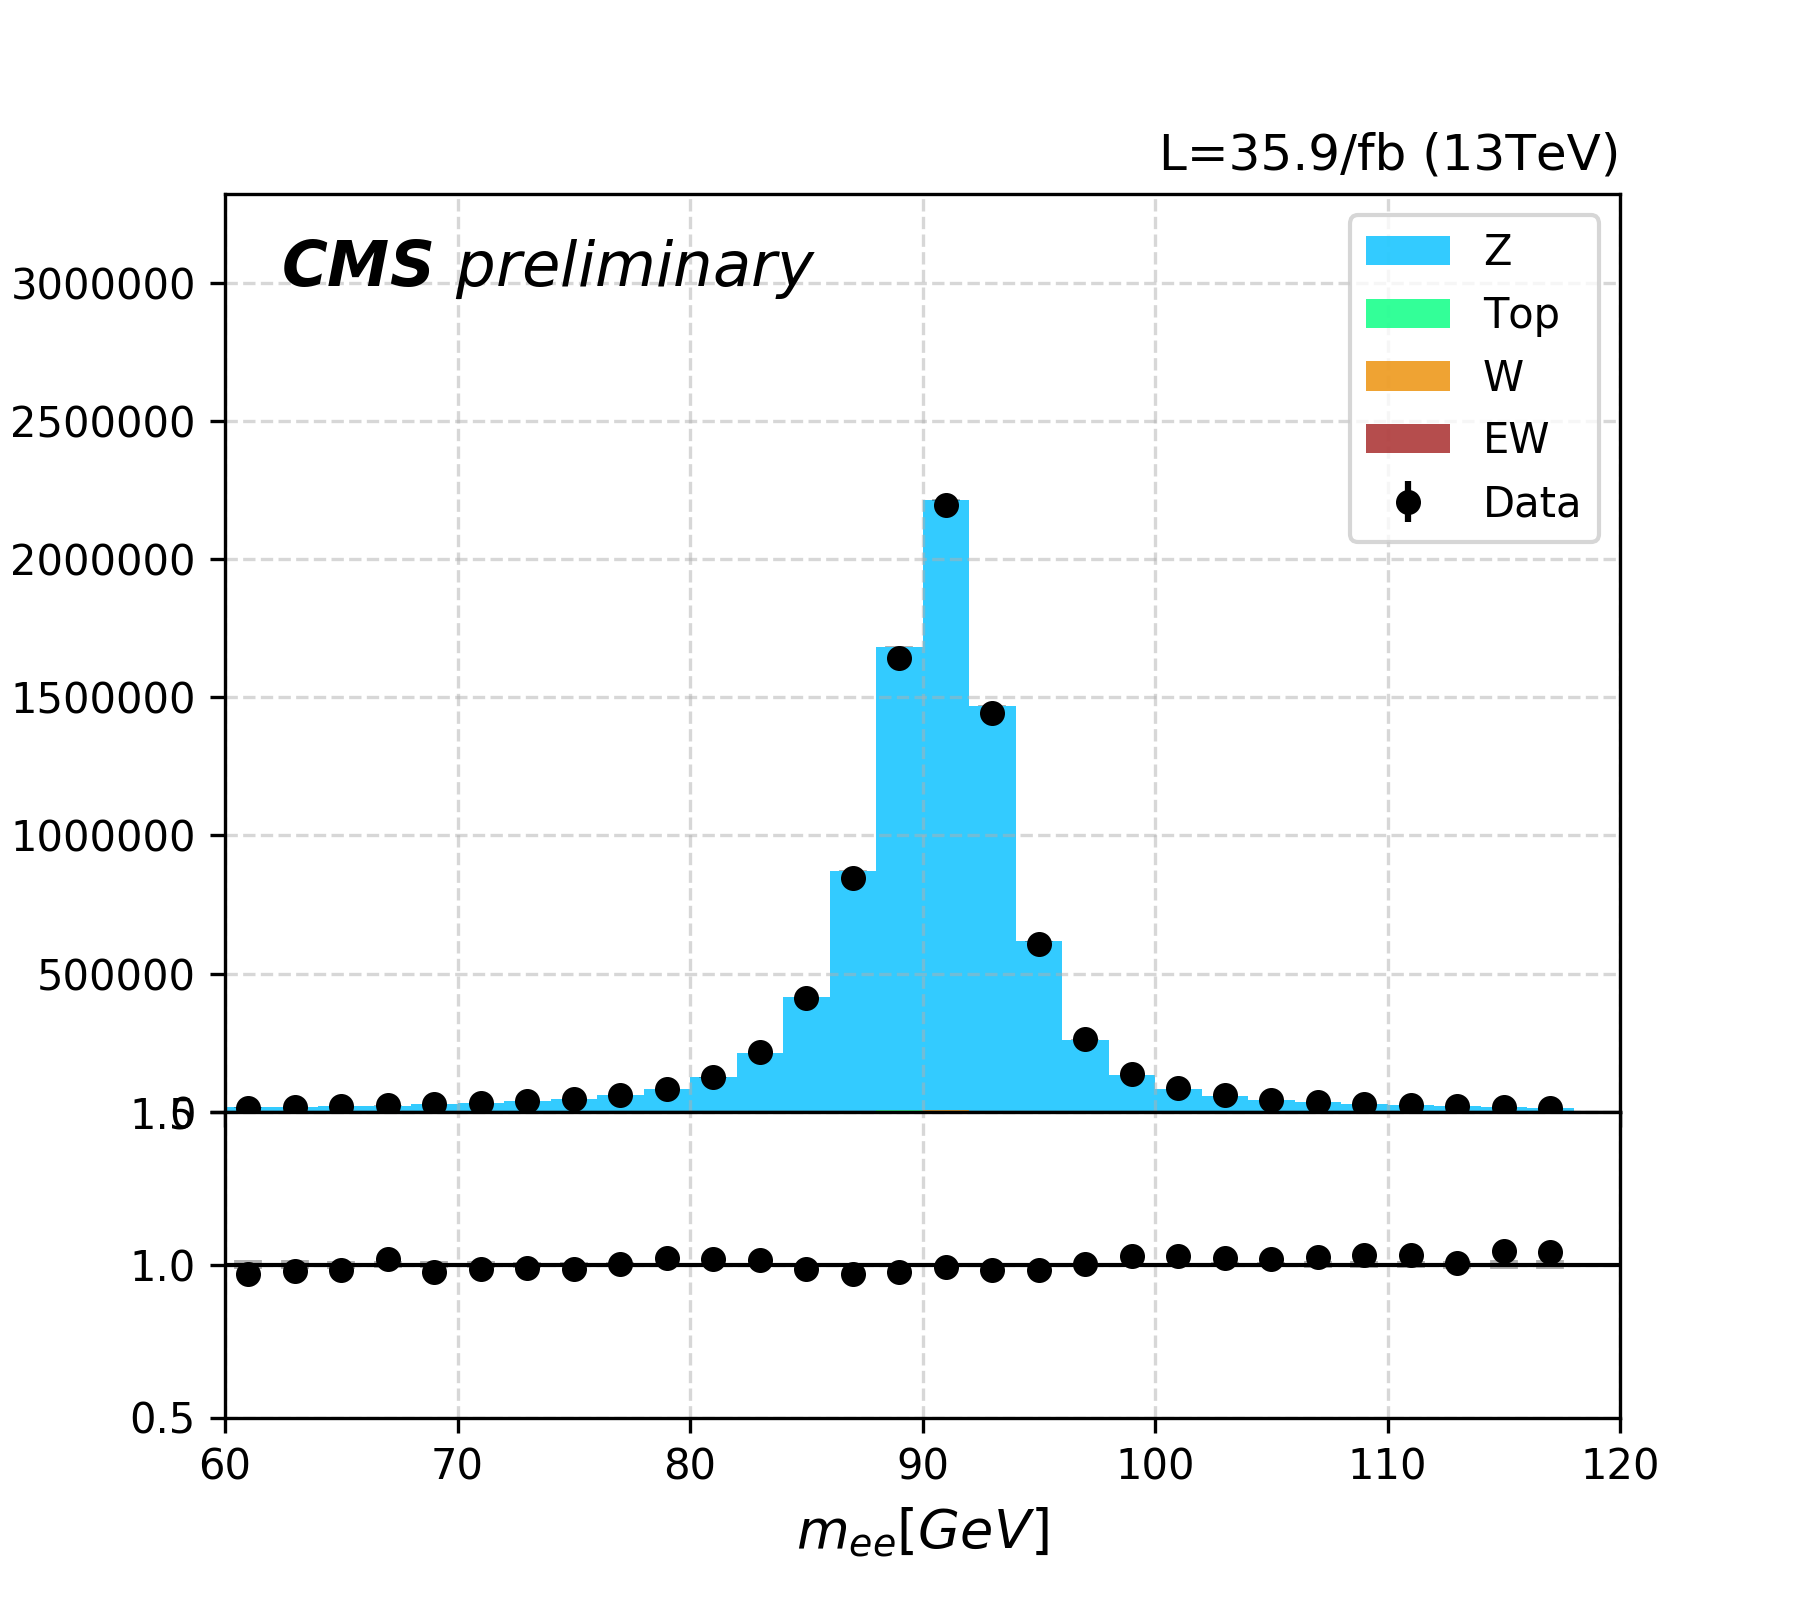
\includegraphics[width=\textwidth]{chapters/Analysis/sectionCalibration/figures/eTrigger/dileptonMass_tag30.png}
        \end{block}
        \begin{center}
            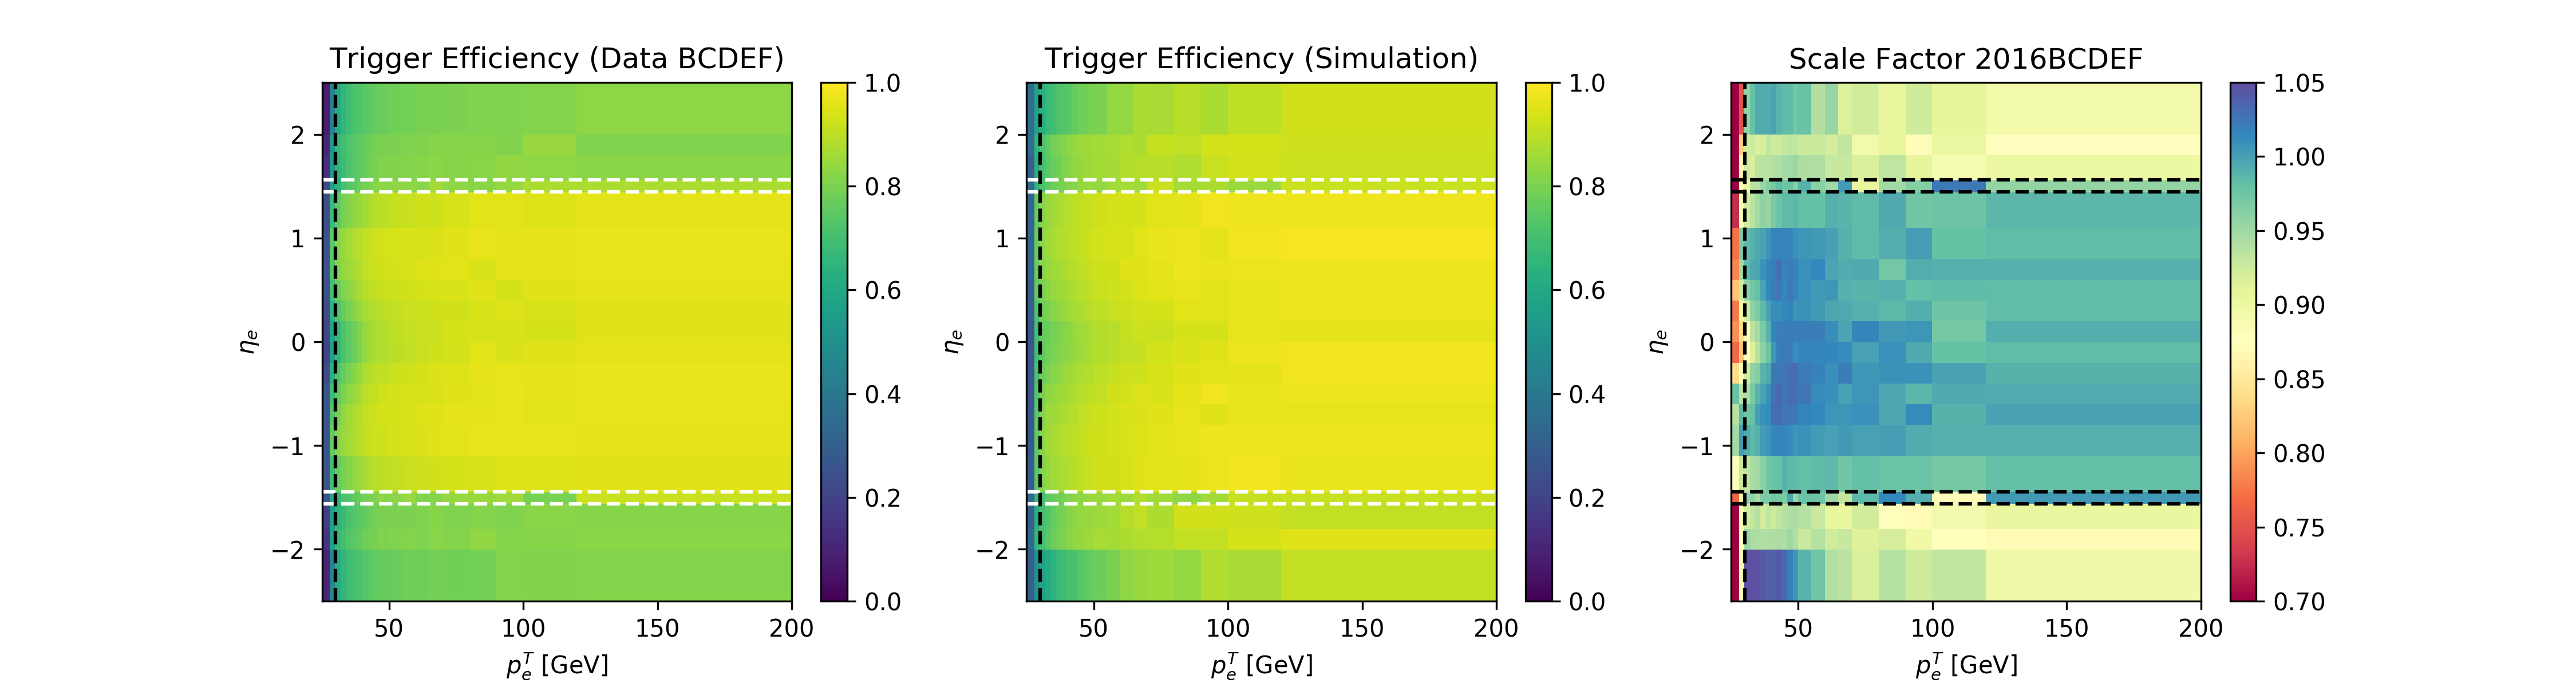
\includegraphics[width=0.49\textwidth, trim=24cm 0 3.7cm 0, clip]{chapters/Analysis/sectionCalibration/figures/eTrigger/eff2d_BCDEF.png}
            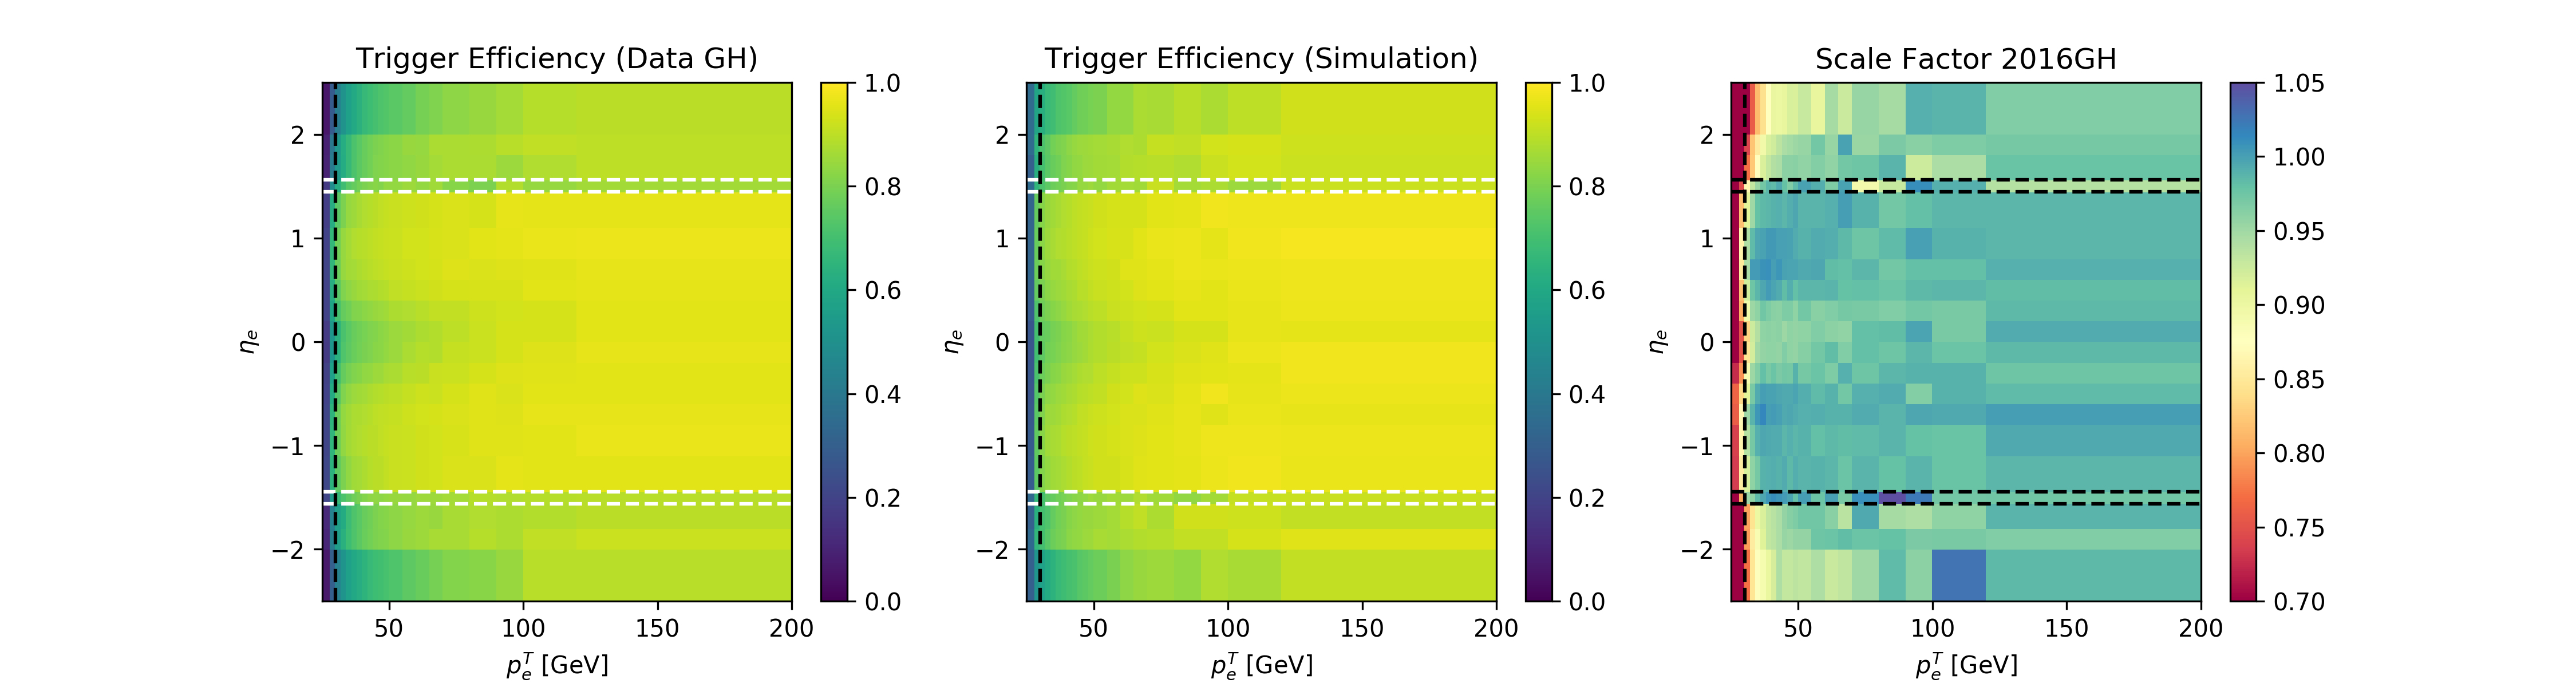
\includegraphics[width=0.49\textwidth, trim=24cm 0 3.7cm 0, clip]{chapters/Analysis/sectionCalibration/figures/eTrigger/eff2d_GH.png}
        \end{center}
    
    \end{columns}
    

\end{frame}



% -------------
% new frame
% -------------
\begin{frame}{$j\to \PGth$ mis-identification}
\smaller \smaller
    \begin{columns}
        \column{0.35\textwidth}
        \begin{block}{\smaller \cmt with $n_j\geq2$, $n_b=1$}
        \centering
            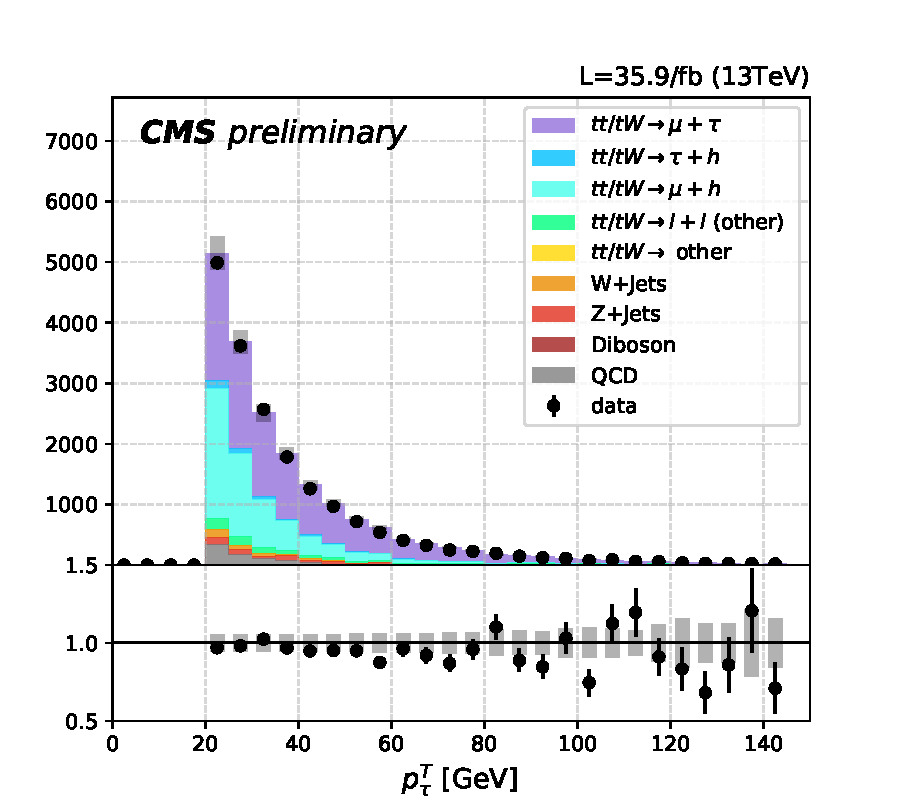
\includegraphics[width=\textwidth]{slides/figures/mutau_1b_lepton2_pt.pdf}
            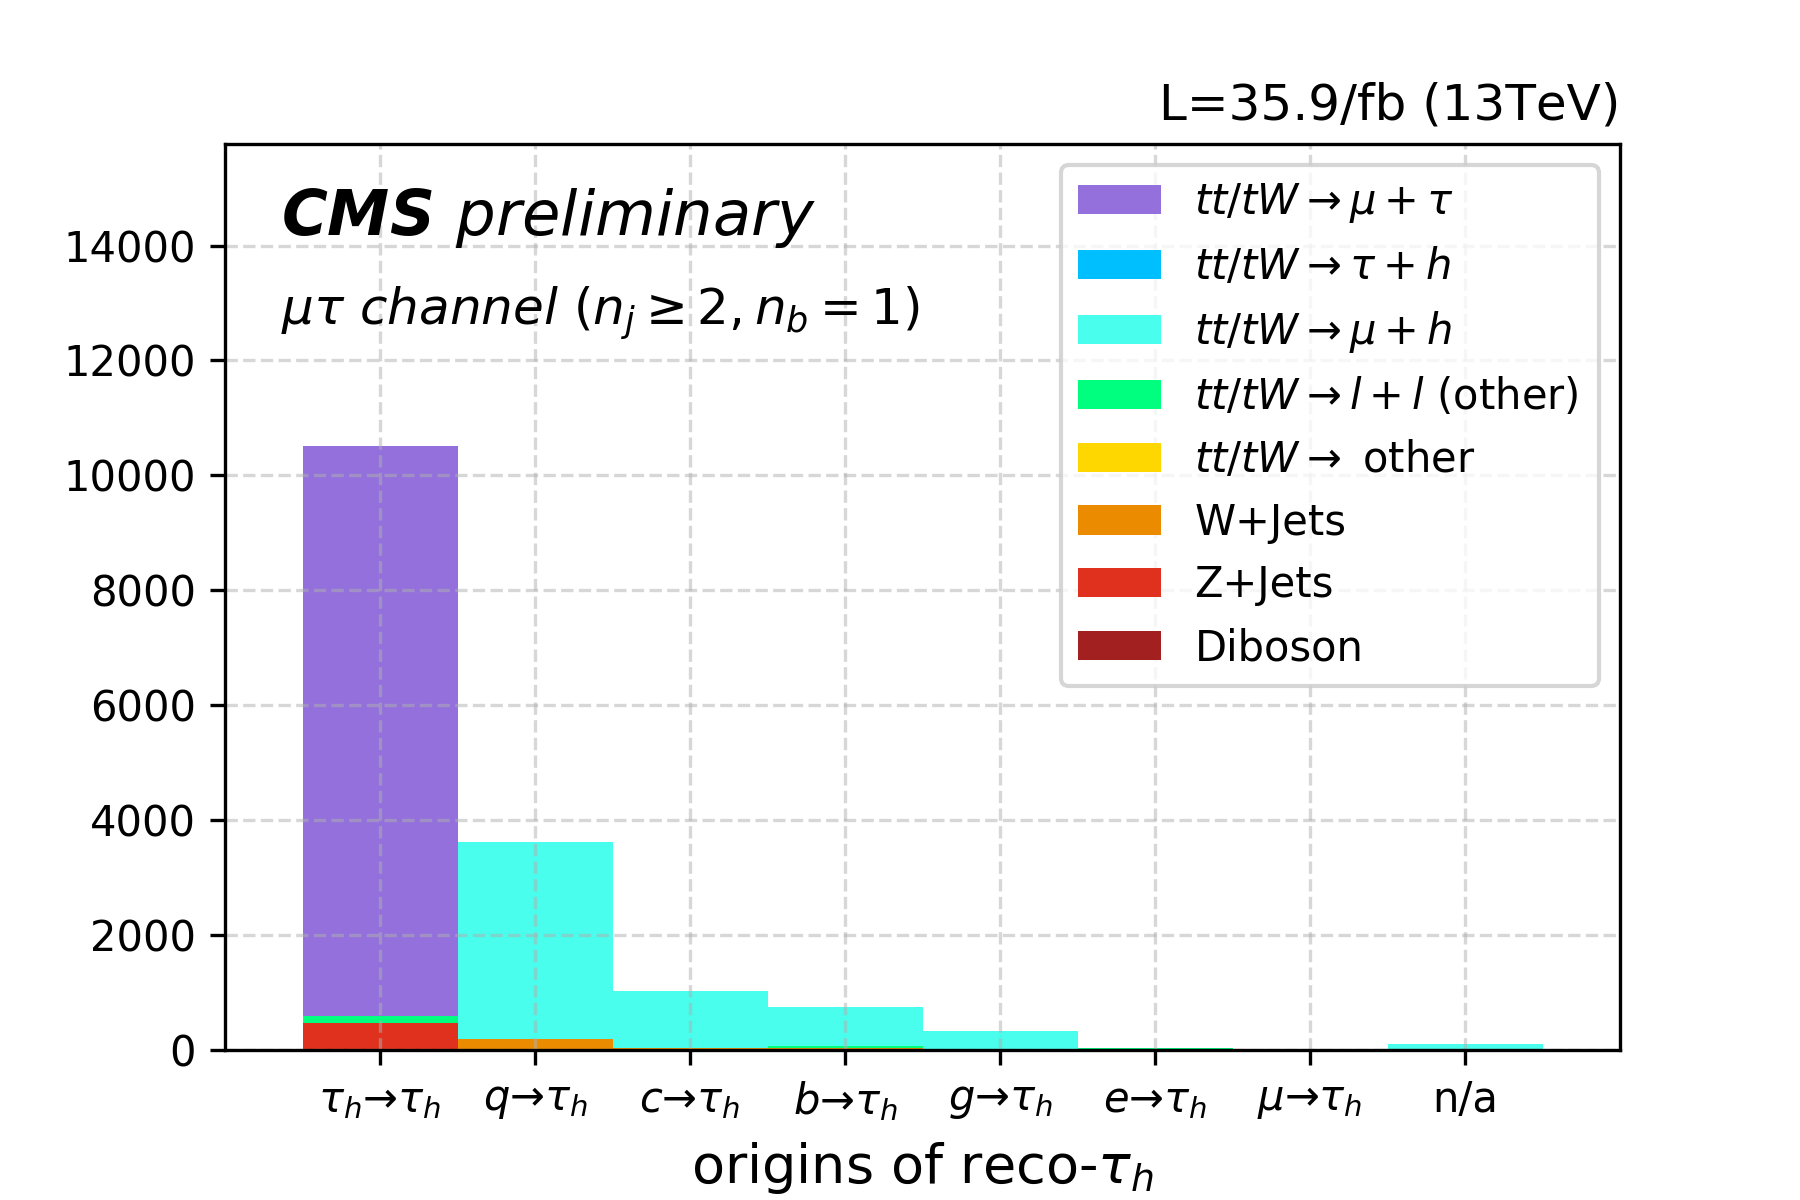
\includegraphics[width=\textwidth]{slides/figures/origin_mutau_1b.png}
        \end{block}
        
        \column{0.55\textwidth}
        \begin{itemize}
            \item Perform a customized measurement of scale factors accounting for the difference of the $j\to \PGth$ fake rate in data and simulation.
            \item $SF_{j \to \PGth}(\pt)$ is measured in $j \to \PGth$ enriched regions:
            \begin{itemize}
            \smaller
                \item \alert{$\cee/\cmm + \PGth$} dominated by \zjets, enriched with light jet faking \PGth;
                \item \alert{$\cem + \PGth$} dominated by \ttbar, enriched with b jet faking \PGth.
            \end{itemize}
            \item The origins of \PGth are found by matching with gen-level particles.
            \item Both Tight and VTight \PGth identification working points are considered.
            \item Systematic uncertainties include luminosity, cross-sections, \Pe/\PGm selection efficiencies.
        \end{itemize}
        \begin{center}
           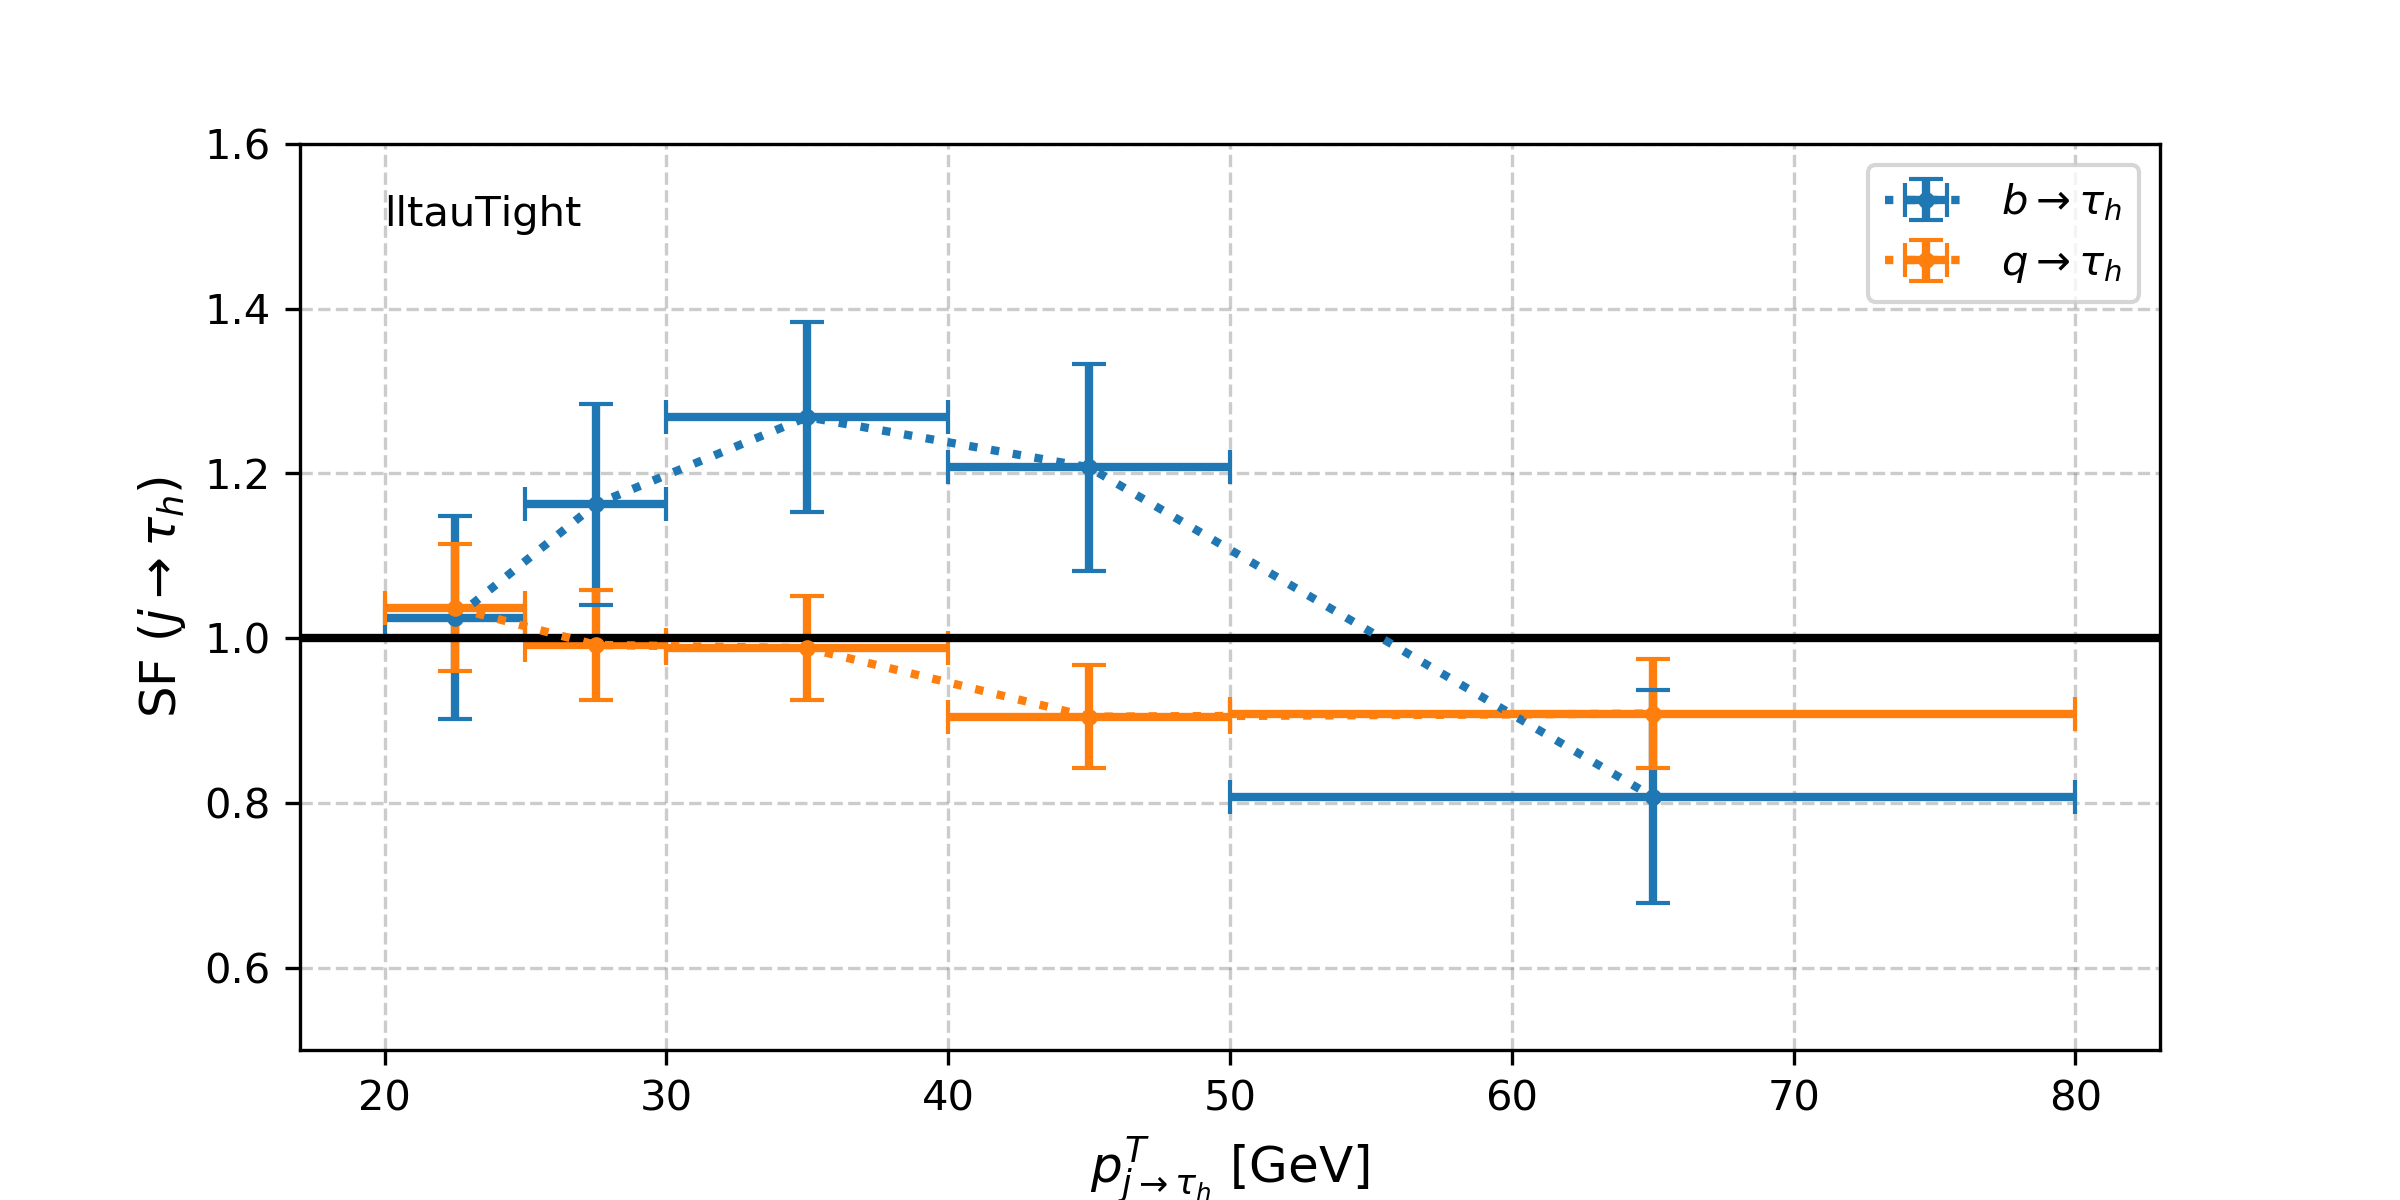
\includegraphics[width=0.8\textwidth]{chapters/Analysis/sectionCalibration/figures/jetToTauh/fit2_ptflavor2_lltauTight.png} 
        \end{center}
        
        
    \end{columns}
    
\end{frame}



\subsection{QCD Estimation}

\begin{frame}{QCD estimation}
\smaller \smaller
    \begin{block}{\cmt and \cet}
    \begin{columns}[c]
        \column{0.7\textwidth}
        \begin{itemize}
            \item Estimated by $n_{\rm data} - \sum n_{\rm MC}$ in the side-band region with \textcolor{red}{same-sign} leptons.
            \item Scale the estimation with a transfer factor \textcolor{blue}{$SF^{\rm SS \to OS}$} measured separately in orthogonal regions: 
            \begin{itemize} 
            \smaller
                \item counting: $\ell \PGth$ with $n_j\geq2,n_b=0$;
                \item shape: $\ell \PGth$ with anti-iso $\ell$ and $n_j=0,n_b=0$.
            \end{itemize}
            % \item Assign 25\% uncertainty to the normalization. [double c]
        \end{itemize}
        
        \column{0.3\textwidth}
        \centering
        \cmt $n_j=0,n_b=0$
        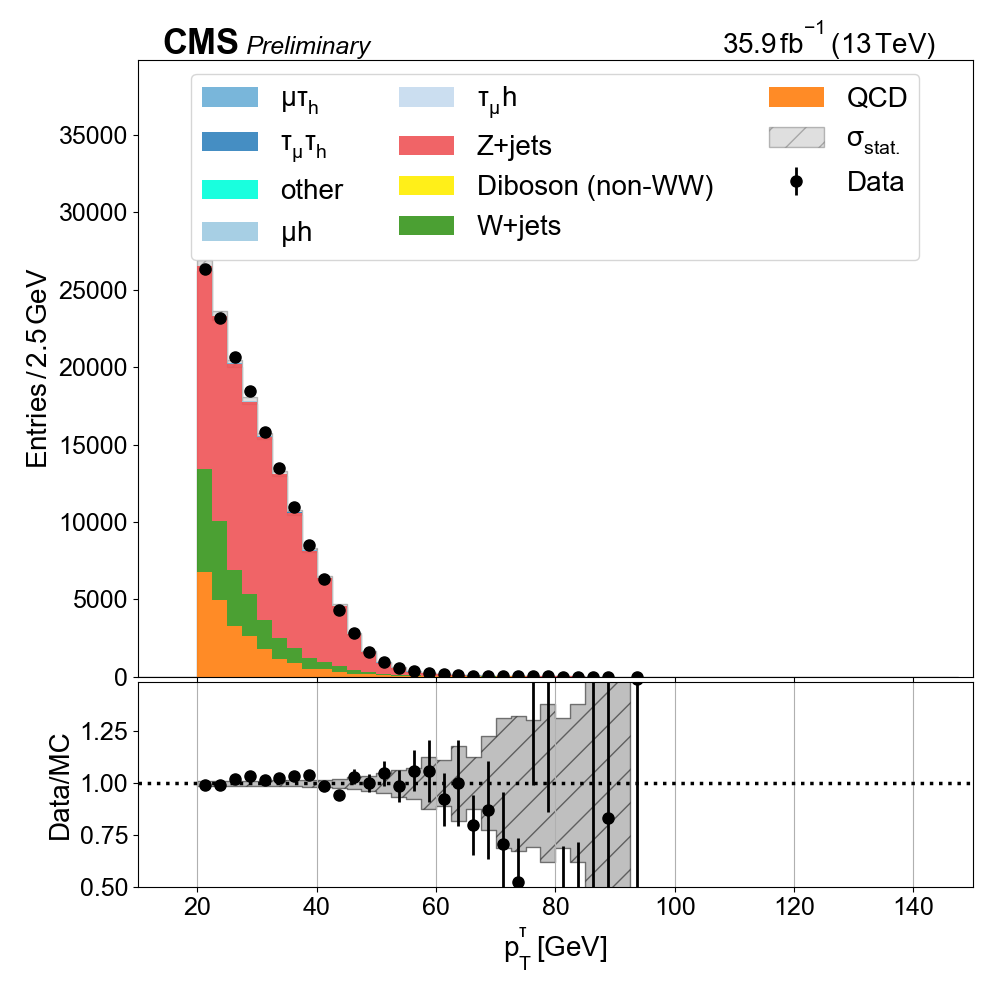
\includegraphics[width=0.8\textwidth]{chapters/Analysis/sectionPlots/figures/data_mc_overlays/mutau_2016_cat_eq0_eq0_signal_linear_lepton_lepton2_pt.png}
    \end{columns}
    \end{block}
    
    

    \begin{block}{\cmh and \ceh}
    \begin{columns}[c]
        \column{0.7\textwidth}
    
        \begin{itemize}
            \item Estimated by $n_{\rm data} - \sum n_{\rm MC}$ in the side-band region with \textcolor{red}{anti-isolated} leptons.
            \item Anti-isolated leptons requires passing Loose but not Tight isolation working point.
            \item Scale the estimation with a transfer factor \textcolor{blue}{ $SF^{\rm \overline{iso} \to iso} (\pt, \eta)$}, measured separately in orthogonal regions ($\ell h$ with $1\leq n_j \leq3, n_b=1$).
            % \item ??? estimation in \ceh is re-normalized by HT-binned QCD ???
            % \item Assign 25\% uncertainty to the normalization. 
        \end{itemize}
        
        \column{0.3\textwidth}
        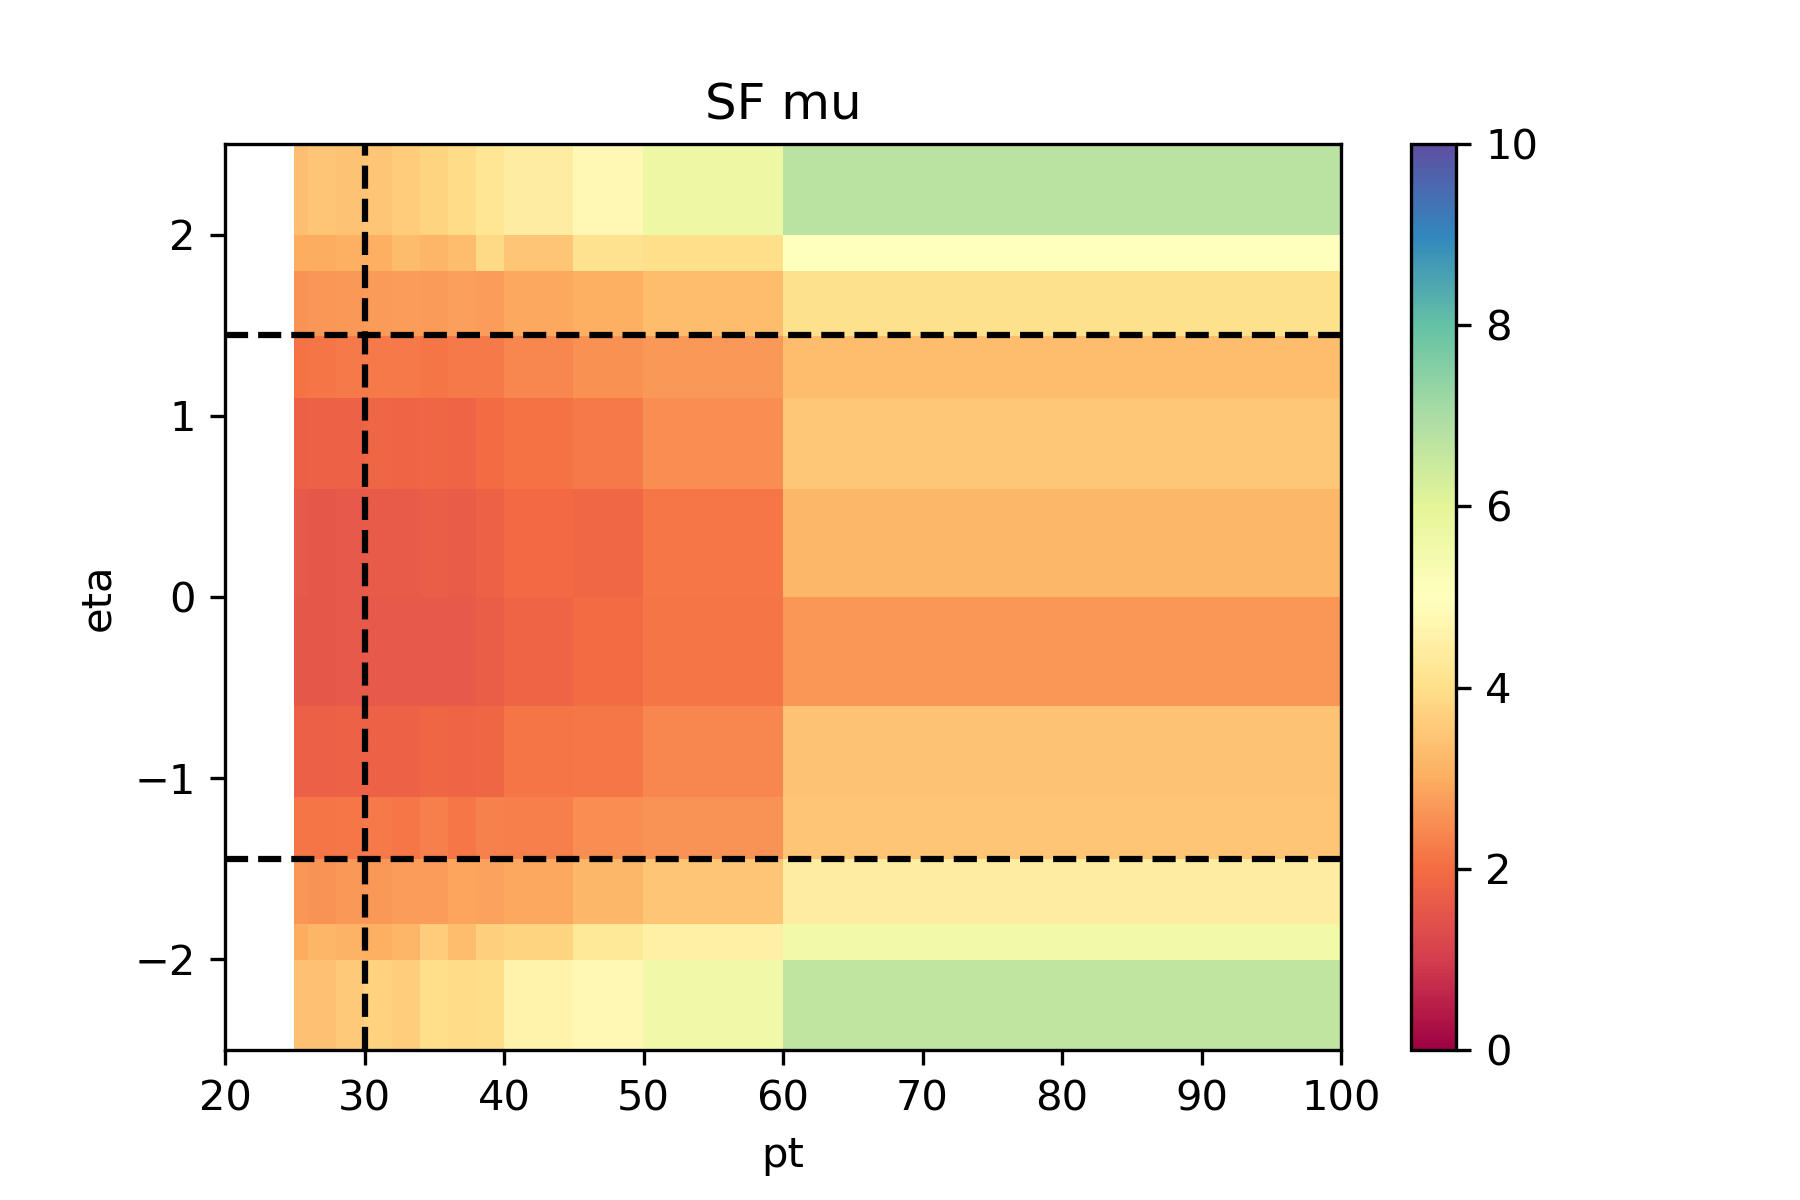
\includegraphics[width=0.95\textwidth,trim=0 0 2cm 0, clip]{chapters/Analysis/sectionBackground/figures/ljets_kinematics/123j1b/SF_mu_2d.png}
        
    \end{columns}
    \end{block}
    
\end{frame}

    
    

    % \begin{center}
    %     \includegraphics[width=0.9\textwidth, trim=0 21cm 32cm 18cm, clip]{chapters/Analysis/sectionBackground/figures/ltau_kinematics/ltau2.png}
    % \end{center}
    
    % normalization from 2j0b and iso-0j0b










\section{Methods of $B(W \to \ell \nu)$ extraction}

\subsection{parameterize WW decay}


\begin{frame}{Parameterize WW decay}

    The important parameters in our signal model are the W branching fractions,
    $$\vbw = \{\bwe, \bwm, \bwt, \bwh\},$$

    subject to the unitary constraint. Taking into account the \PGt decay modes, $\{\bte, \btm, \bth\}$, the \PW decay modes can be split further,

    $$\vbw^\prime = \{\bwe, \bwm, \bwt\bte, \bwt\btm, \bwt\bth, \bwh\}. $$

    All the possible terms for WW decays can be written in a matrix formed by the
    outer product of $\vbw^\prime$,

    \begin{equation*}
    \footnotesize
    \boldsymbol{B} =  \vbw^\prime\otimes \vbw^\prime =
    \begin{bmatrix}
        \bwe \bwe       & \bwe \bwm         & \bwe \bwt \bte        & \bwe \bwt \btm        & \bwe \bwt \bth        & \bwe \bwh         \\
        \bwm \bwe       & \bwm \bwm         & \bwm \bwt \bte        & \bwm \bwt \btm        & \bwm \bwt \bth        & \bwm \bwh         \\
        \bwt \bte \bwe  & \bwt \bte \bwm    & \bwt \bte \bwt \bte   & \bwt \bte \bwt \btm   & \bwt \bte \bwt \bth   & \bwt \bte \bwh    \\
        \bwt \btm \bwe  & \bwt \btm\bwm     & \bwt \btm \bwt \bte   & \bwt \btm \bwt \btm   & \bwt \btm \bwt \bth   & \bwt \btm \bwh    \\
        \bwt \bth \bwe  & \bwt \bth \bwm    & \bwt \bth \bwt \bte   & \bwt \bth \bwt \btm   & \bwt \bth \bwt \bth   & \bwt \bth \bwh    \\
        \bwh \bwe       & \bwh \bwm         & \bwh \bwt \bte        & \bwh \bwt \btm        & \bwh \bwt \bth        & \bwh  \bwh 
	\end{bmatrix} 
	\end{equation*}

    This is a six-by-six symmetric matrix.

\end{frame}

% -------------
% new frame
% -------------
\begin{frame}{}
    Correspondingly, there is a $6\times6$ symmetric matrix of the efficiencies\footnotemark for each decay mode to contribute to a specific final state,
    \begin{columns}
        \column{0.6\textwidth}
        \begin{equation*}
        \footnotesize
        \boldsymbol{E} = \begin{bmatrix}
            \epsilon_{\Pe\Pe}       & \epsilon_{\Pe\PGm}        & \epsilon_{\Pe\PGte}       & \epsilon_{\Pe\PGtmu}          & \epsilon_{\Pe\PGth}       & \epsilon_{\Pe \mathrm{h}}   \\
            \epsilon_{\Pe\PGm}      & \epsilon_{\PGm\PGm}       & \epsilon_{\PGm\PGte}      & \epsilon_{\PGm\PGtmu}         & \epsilon_{\PGm\PGth}      & \epsilon_{\PGm \mathrm{h}}  \\
            \epsilon_{\Pe\PGte}     & \epsilon_{\PGm\PGte}      & \epsilon_{\PGte\PGte}     & \epsilon_{\PGte\PGtmu}        & \epsilon_{\PGte\PGth}     & \epsilon_{\PGte \mathrm{h}} \\
            \epsilon_{\Pe\PGtmu}    & \epsilon_{\PGm\PGtmu}     & \epsilon_{\PGte\PGtmu}    & \epsilon_{\PGtmu\PGtmu}       & \epsilon_{\PGtmu\PGth}    & \epsilon_{\PGtmu \mathrm{h}}\\
            \epsilon_{\Pe\PGth}     & \epsilon_{\PGm\PGth}      & \epsilon_{\PGte\PGth}     & \epsilon_{\PGtmu\PGth}        & \epsilon_{\PGth\PGth}     & \epsilon_{\PGth \mathrm{h}} \\
            \epsilon_{\Pe\mathrm{h}}& \epsilon_{\PGm\mathrm{h}} & \epsilon_{\PGte\mathrm{h}}& \epsilon_{\PGtmu\mathrm{h}}   & \epsilon_{\PGth\mathrm{h}}& \epsilon_\mathrm{hh}        \\
        \end{bmatrix},
        \end{equation*}
        
        \column{0.4\textwidth}
        % \begin{tcolorbox}{}
        \smaller
        where the efficiencies are determined from simulated events,
        \begin{equation*}
            \epsilon = \frac{\sum_{\sf i\in acc.}w_{i}}{N_{total}}.
        \end{equation*}
        The prediction of signal events is,
        \begin{equation*}
            n_{s} = \sigma_{s} \mathcal{L} \mathbf{E}_{ij} \mathbf{B}_{ij}. 
        \end{equation*}
        % \end{tcolorbox}
    \end{columns}
    
    \vspace{0.05\textheight}
    \begin{center}
        \includegraphics[width=0.8\textwidth,trim=3cm 0 3cm 0, clip]{chapters/Analysis/sectionStatisticalAnalysis/figures/acc_mu1b.png}
        % \includegraphics[width=0.7\textwidth]{chapters/Analysis/sectionStatisticalAnalysis/figures/acc_mu2b.png}
        % \includegraphics[width=0.7\textwidth]{chapters/Analysis/sectionStatisticalAnalysis/figures/acc_e1b.png}
        % \includegraphics[width=0.7\textwidth]{chapters/Analysis/sectionStatisticalAnalysis/figures/acc_e2b.png}
    \end{center}

    %\vspace{-0.08in}


    \footnotetext[1]{\alert{\tiny N.B. W+jets accounted for just using the vector $\beta$ and the
    corresponding vector of efficiencies.}}
\end{frame}







\subsection{counting analysis}

% -------------
% new frame
% -------------
\begin{frame}{Counting analysis}
    % \begin{figure}
    %     \centering
    %     \includegraphics[width=0.9\textwidth]{chapters/Analysis/sectionStatisticalAnalysis/figures/counting.png}
    % \end{figure}

    \smaller
    For each of the trigger and $n_b$ regions, construct ratios \textcolor{NUpurple}{$\{X_{e},X_{\mu},X_{\tau}\}$} from data with background subtracted $n = N_{\rm data} - \sum N_{\rm bg}$,
    % Please add the following required packages to your document preamble:

    \begin{table}[]
        \centering
        \setlength{\tabcolsep}{2.5 em}
        \renewcommand{\arraystretch}{3}
        \resizebox{0.9\textwidth}{!}{
        \begin{tabular}{c|c|c|c|c}
        \rowcolor{NUpurple} 
                                & \multicolumn{2}{c|}{\textcolor{white}{Single-$\mu$ Trigger}}  & \multicolumn{2}{c}{\textcolor{white}{Single-$e$ Trigger}}    \\
        \rowcolor{NUpurple10} 
                                & $n_b = 1$                    & $n_b \geq 2$                   & $n_b = 1$                          & $n_b \geq 2$     \\ \hline 
        channels                & \multicolumn{2}{c|}{$\mu e$, $\mu \mu$, $\mu \tau_h$, $\mu h$} & \multicolumn{2}{c}{$e e$, $e \mu$, $e \tau_h$, $e h$}\\ \hline 
        \multirow{3}{*}{ratios, $t\in \{ \mu, e\}$} 
                                & \multicolumn{4}{c}{$\frac{n^{\ctre}  }{n^{\ctre} + n^{\ctrm} + n^{t\PGt} + n^{\ctrh}} = \textcolor{RedOrange}{X_\Pe   = \frac{ \Eij^{\ctre}\Bij }{  \Eij^{\ctre}\Bij+ \Eij^{\ctrm}\Bij+ \Eij^{t\PGt}\Bij+ \Eij^{\ctrh}\Bij}}$}\\
                                & \multicolumn{4}{c}{$\frac{n^{\ctrm}  }{n^{\ctre} + n^{\ctrm} + n^{t\PGt} + n^{\ctrh}} = \textcolor{Blue}{X_\PGm  = \frac{ \Eij^{\ctrm}\Bij }{  \Eij^{\ctre}\Bij+ \Eij^{\ctrm}\Bij+ \Eij^{t\PGt}\Bij+ \Eij^{\ctrh}\Bij}}$} \\
                                & \multicolumn{4}{c}{$\frac{n^{t\PGt}  }{n^{\ctre} + n^{\ctrm} + n^{t\PGt} + n^{\ctrh}} = \textcolor{OliveGreen}{X_\PGt  = \frac{ \Eij^{t\PGt}\Bij }{  \Eij^{\ctre}\Bij+ \Eij^{\ctrm}\Bij+ \Eij^{t\PGt}\Bij+ \Eij^{\ctrh}\Bij}}$} 
        \end{tabular}
        }
    \end{table}
    
   
\end{frame}



% -------------
% new frame
% -------------
\begin{frame}{}%Frame Title}
\smaller

    One gets a system of three quadratic equations with three unknowns $\{\bwe,\bwm,\bwt\}$,

    \begin{equation*}
    \tiny
	\begin{split}
        \textcolor{RedOrange}{F_\Pe(\bwe,\bwm,\bwt)} = c_{\Pe1} \bwe^2 + c_{\Pe2} \bwm^2 + c_{\Pe3} \bwt^2 + c_{\Pe4} \bwe\bwm + c_{\Pe5} \bwe\bwt + c_{\Pe6} \bwm\bwt + c_{\Pe7} \bwe + c_{\Pe8} \bwm + c_{\Pe9} \bwt + c_{\Pe0} &= 0 ,\\
        \textcolor{Blue}{F_\PGm(\bwe,\bwm,\bwt)} = c_{\PGm 1} \bwe^2 + c_{\PGm 2} \bwm^2 + c_{\PGm 3} \bwt^2 + c_{\PGm 4} \bwe\bwm + c_{\PGm 5} \bwe\bwt + c_{\PGm 6} \bwm\bwt + c_{\PGm 7} \bwe + c_{\PGm 8} \bwm + c_{\PGm 9} \bwt + c_{\PGm 0} &= 0, \\
        \textcolor{OliveGreen}{F_\PGt(\bwe,\bwm,\bwt)} = c_{_\PGt1} \bwe^2 + c_{\PGt2} \bwm^2 + c_{\PGt3} \bwt^2 + c_{\PGt4} \bwe\bwm + c_{\PGt5} \bwe\bwt + c_{\PGt6} \bwm\bwt + c_{\PGt7} \bwe + c_{\PGt8} \bwm + c_{\PGt9} \bwt + c_{\PGt0} &= 0 , \\
    \end{split}
    \end{equation*}
    
    where the coefficients $\{c_{ek},c_{\mu k},c_{\tau k} \}$ with $k\in\{ 0,1,2,\dots 9\}$ are fully determined by efficiencies $E$ and data ratios $\{X_e,X_\mu,X_\tau\}$.


	\begin{columns}[c] % align columns

	\column{.45\textwidth}
		\begin{figure}
			\centering
			\includegraphics[width=0.9\textwidth]{chapters/Analysis/sectionStatisticalAnalysis/figures/visual.png}
		\end{figure}


	\column{.55\textwidth}
    \begin{itemize}
        \item In the $\{\beta_{e},\beta_{\mu},\beta_{\tau}\}$ space, three quadratic equations are three hyperbolic planes, intersection of which is the solution.
		\begin{equation*} 
            \small
            \begin{bmatrix} \bwe \\ \bwm \\ \bwt \end{bmatrix} = \text{Sol} 
                \begin{bmatrix}
                \textcolor{RedOrange}{F_\Pe (\bwe,\bwm,\bwt) = 0} \\
                \textcolor{Blue}{F_\PGm  (\bwe,\bwm,\bwt) = 0} \\
                \textcolor{OliveGreen}{F_\PGt (\bwe,\bwm,\bwt) = 0}
                \end{bmatrix}
		\end{equation*}
        \item The results from four different data categories are analytically combined considering the uncorrelated statistical error and correlated systematic errors.  
        \end{itemize}

	\end{columns}

\end{frame}





\subsection{shape analysis}

\begin{frame}{Shape analysis}
\smaller 
    \begin{columns}
        \column{0.6\textwidth}
        \begin{block}{\smaller discriminating $W\rightarrow e/\mu$ vs. $W\rightarrow\tau\rightarrow e/\mu$}
            \begin{itemize}
                \item Features are selected to best isolate
                    $W\rightarrow\tau$ decays 
                \begin{itemize}
                \smaller
                    \item \alert{$W\rightarrow\tau\rightarrow e/\mu$ tend to have lower \pt}
                \end{itemize}
                \item More sophisticated discrimination techniques considered, e.g.
                    neural networks, but...
                \begin{itemize}
                \smaller
                    \item lepton $\pt$ is by far still strongest source of discrimination
                    \item additional observables complicates accounting for systematic uncertainties
                \end{itemize}
                \item Trailing muon impact parameter considered (as for ATLAS), but was poorly calibrated
                \item Histograms binning are generated using the Bayesian Block algorithm (arXiv:1708.00810)
            \end{itemize}

        \end{block}


        \column{0.4\textwidth}
        \begin{center}
            % \vspace{-0.1in} 
            \includegraphics[width=0.9\textwidth]{chapters/Analysis/sectionPlots/figures/kinematics_pickles/mumu/12b/mumu_2b_lepton2_pt.pdf}
            \includegraphics[width=0.9\textwidth]{chapters/Analysis/sectionSelection/figures/sob/mumu_lepton2_d0_logscale.pdf}
        \end{center}

    \end{columns}

\end{frame}


\begin{frame}{}
\smaller 

    \begin{block}{\smaller binned maximum likelihood estimation}
        In this case, the W branching fractions, $\mathbf{B}$, are treated as free parameters, and the values that minimize the NLL assuming Poisson probabilities are determined,

        \begin{equation*}
            \mathsf{NLL}(\boldsymbol{B}, \boldsymbol{\theta}|\mathbf{y}) = \sum_{\mathsf{i\in category}} 
            \sum_{\mathsf{j \in bins}} -y_{ij}\ln(f_{ij}(\boldsymbol{B}, \boldsymbol{\theta})) + f_{ij}(\boldsymbol{B}, \boldsymbol{\theta}) + \sum_{k\in n.p.}\pi_\theta (\theta)
        \end{equation*}

        where $y_{ij}$ is the data yield in category $i$ and bin $j$, and $f_{ij}$ is the prediction
        parameterized by the branching fractions, $\mathbf{B}$ and nuisance parameters,
        $\boldsymbol{\theta}$. The constraint on the n.p. are denoted by $\pi_{\theta}(\theta)$. The
        data model is written, 

        \begin{equation*}
            f_{ij}(\boldsymbol{B}, \boldsymbol{\theta}) = \sum_{s\in sig} s_{ij,s}(\boldsymbol{B}, \boldsymbol{\theta}) + \sum_{b\in bg} b_{ij,b}(\boldsymbol{\theta}). 
        \end{equation*}

    \end{block}

    \begin{itemize}
        \smaller
        \item 30 categories based on jet and b tag multiplicities 
        \item total of 72 template components, w/ only $\sim 10$ are relevant to any specific category
        \item $\sim 100$ non-MC stat nuisance parameters
        \item $\sim 400$ bins in total 
        \item template morphing and MC stat. variation implemented according to arXiv:1103.0354
        \item minimization using \textcolor{blue}{\texttt{scipy.optimize.minimize}}
    \end{itemize}
    
\end{frame}



\begin{frame}{} %$ee$ and $\mu\mu$: trailing lepton $\pt$}
Post-fit distributions

    \begin{columns}
        \column{0.5\textwidth}
        \begin{tcolorbox}[colframe=NUpurple]{ \cee and \cmm: trailing lepton $\pt$}
            \begin{center}
                \includegraphics[width=0.48\textwidth]{chapters/Analysis/sectionStatisticalAnalysis/figures/fit/ee_cat_gt2_eq1_b}
                \includegraphics[width=0.48\textwidth]{chapters/Analysis/sectionStatisticalAnalysis/figures/fit/ee_cat_gt2_gt2_b}

                \includegraphics[width=0.48\textwidth]{chapters/Analysis/sectionStatisticalAnalysis/figures/fit/mumu_cat_gt2_eq1_b}
                \includegraphics[width=0.48\textwidth]{chapters/Analysis/sectionStatisticalAnalysis/figures/fit/mumu_cat_gt2_gt2_b}
            \end{center}
        \end{tcolorbox}{}

        \column{0.5\textwidth}
        \begin{tcolorbox}[colframe=NUpurple]{ \ceh and \cmh: lepton $\pt$}
            \begin{center}
                \includegraphics[width=0.48\textwidth]{chapters/Analysis/sectionStatisticalAnalysis/figures/fit/ejet_cat_gt4_eq1}
                \includegraphics[width=0.48\textwidth]{chapters/Analysis/sectionStatisticalAnalysis/figures/fit/ejet_cat_gt4_gt2}

                \includegraphics[width=0.48\textwidth]{chapters/Analysis/sectionStatisticalAnalysis/figures/fit/mujet_cat_gt4_eq1}
                \includegraphics[width=0.48\textwidth]{chapters/Analysis/sectionStatisticalAnalysis/figures/fit/mujet_cat_gt4_gt2}
            \end{center}
        \end{tcolorbox}
    \end{columns}

\end{frame}

\begin{frame}{}
Post-fit distributions
    \begin{tcolorbox}[colframe=NUpurple]{ \cem: trailing lepton $\pt$}
        \begin{center}
            \includegraphics[width=0.25\textwidth]{chapters/Analysis/sectionStatisticalAnalysis/figures/fit/emu_cat_eq0_eq0_a}
            \includegraphics[width=0.25\textwidth]{chapters/Analysis/sectionStatisticalAnalysis/figures/fit/emu_cat_eq1_eq0_a}
            \includegraphics[width=0.25\textwidth]{chapters/Analysis/sectionStatisticalAnalysis/figures/fit/emu_cat_eq1_eq1_a}

            \includegraphics[width=0.25\textwidth]{chapters/Analysis/sectionStatisticalAnalysis/figures/fit/emu_cat_gt2_eq0}
            \includegraphics[width=0.25\textwidth]{chapters/Analysis/sectionStatisticalAnalysis/figures/fit/emu_cat_gt2_eq1_a}
            \includegraphics[width=0.25\textwidth]{chapters/Analysis/sectionStatisticalAnalysis/figures/fit/emu_cat_gt2_gt2_a}
        \end{center}
    \end{tcolorbox}

\end{frame}

\begin{frame}{}
Post-fit distributions
    \begin{tcolorbox}[colframe=NUpurple]{ \cet: tau $\pt$}
        \begin{center}
            \includegraphics[width=0.24\textwidth]{chapters/Analysis/sectionStatisticalAnalysis/figures/fit/etau_cat_eq0_eq0}
            \includegraphics[width=0.24\textwidth]{chapters/Analysis/sectionStatisticalAnalysis/figures/fit/etau_cat_eq1_eq0}
            \includegraphics[width=0.24\textwidth]{chapters/Analysis/sectionStatisticalAnalysis/figures/fit/etau_cat_gt2_eq0}
            \includegraphics[width=0.24\textwidth]{chapters/Analysis/sectionStatisticalAnalysis/figures/fit/etau_cat_eq1_eq1}

            \includegraphics[width=0.24\textwidth]{chapters/Analysis/sectionStatisticalAnalysis/figures/fit/etau_cat_eq2_eq1}
            \includegraphics[width=0.24\textwidth]{chapters/Analysis/sectionStatisticalAnalysis/figures/fit/etau_cat_eq2_eq2}
            \includegraphics[width=0.24\textwidth]{chapters/Analysis/sectionStatisticalAnalysis/figures/fit/etau_cat_gt3_eq1}
            \includegraphics[width=0.24\textwidth]{chapters/Analysis/sectionStatisticalAnalysis/figures/fit/etau_cat_gt3_gt2}
        \end{center}
    \end{tcolorbox}
\end{frame}

\begin{frame}{}
Post-fit distributions
    \begin{tcolorbox}[colframe=NUpurple]{ \cmt: tau $\pt$}
        \begin{center}
            \includegraphics[width=0.24\textwidth]{chapters/Analysis/sectionStatisticalAnalysis/figures/fit/mutau_cat_eq0_eq0}
            \includegraphics[width=0.24\textwidth]{chapters/Analysis/sectionStatisticalAnalysis/figures/fit/mutau_cat_eq1_eq0}
            \includegraphics[width=0.24\textwidth]{chapters/Analysis/sectionStatisticalAnalysis/figures/fit/mutau_cat_gt2_eq0}
            \includegraphics[width=0.24\textwidth]{chapters/Analysis/sectionStatisticalAnalysis/figures/fit/mutau_cat_eq1_eq1}

            \includegraphics[width=0.24\textwidth]{chapters/Analysis/sectionStatisticalAnalysis/figures/fit/mutau_cat_eq2_eq1}
            \includegraphics[width=0.24\textwidth]{chapters/Analysis/sectionStatisticalAnalysis/figures/fit/mutau_cat_eq2_eq2}
            \includegraphics[width=0.24\textwidth]{chapters/Analysis/sectionStatisticalAnalysis/figures/fit/mutau_cat_gt3_eq1}
            \includegraphics[width=0.24\textwidth]{chapters/Analysis/sectionStatisticalAnalysis/figures/fit/mutau_cat_gt3_gt2}
        \end{center}
    \end{tcolorbox}

\end{frame}

\section{Systematic Uncertainties}



\begin{frame}{Handling systematics}

    \begin{itemize}
        \item Statistical uncertainties are calculated using different approaches for the two analyses.
        \item Shape analysis:
        \begin{itemize}
            \smaller
            \item uncertainty is included in fit with nuisance parameters (n.p.);
            \item most uncertainties are accounted for using morphing templates;
            \item MC statistical uncertainty accounted for on a bin-by-bin basis using Barlow-Beeston approach;
            \item the same systematic parameter in all relevant categories are fully correlated;
            \item different systematic parameters are independent before fit. (correlations are generated by the fitting process.)
        \end{itemize}
        
        \item Counting analysis:
        \begin{itemize}
            \smaller
            \item uncertainty accounted for by carrying out measurement with each uncertainty source varied by $\pm 1\sigma$;
            \item results in different trigger and $n_b$ categories are analytically combined by $\chi^2$ assuming:
            \begin{itemize}
            \smaller 
                \item the same source of systematics is fully correlated;
                \item difference sources of systematics is independent.
            \end{itemize}
        \end{itemize}
    \end{itemize}

\end{frame}


\begin{frame}{Sources of systematic uncertainties}
\smaller

    \begin{itemize}
        \item Luminosity (2.5\%).
        \item Cross-section\footnotemark: \ttbar (5\%), \tW (5\%), \zjets (10\%), \wjets (5\%), \gjets (10\%), VV (10\%). 
        
        \item QCD estimation in $\ell\PGth$ and $\ell h$ (25\%).
        \item Gen-level reweightings: PU, top \pt, \WW \pt .
        \item Trigger efficiencies: single muon trigger, single electron trigger.
        \item Object reconstruction:
        \begin{itemize}
        \smaller
            \item muon: identification, isolation, energy scale.
            \item electron: identification, reconstruction, energy scale.
            \item tau: identification, misidentification, energy scale.
            \item jet: energy scale, energy resolution.
            \item btag: tag/mistag.
        \end{itemize}
        \item Tau decay branching fractions: $\PGt \to \Pe$, $\PGt \to \PGm$, $\PGt \to \mathrm{h}$.
        \item Simulation of \ttbar: ISR/FSR, matrix element to parton shower matching (ME-PS), underlying event tuning (UE).
        
    \end{itemize}

\footnotetext[2]{\footnotesize Shape analysis decomposes \ttbar, \wjets, \zjets cross-sections into generator parameters, e.g. PDF, \alpS, $\mu_f$, $\mu_r$, to avoid constraining relevant n.p..}
\end{frame}





\begin{frame}{}
counting analysis
    \centering
    \includegraphics[width=\textwidth, trim=1.5cm 0cm 3.5cm 1cm, clip]{chapters/Analysis/sectionSystematics/figures/systematics_impact_counting.pdf}
\end{frame}

\begin{frame}{}
shape analysis
    \centering
    \includegraphics[width=\textwidth]{chapters/Analysis/sectionSystematics/figures/pulls_impacts_final.pdf}
\end{frame}










\section{Results}

\begin{frame}{Results}
    \begin{table}[htb!]
        \centering
        \setlength{\tabcolsep}{1.5em}
        \renewcommand{\arraystretch}{1.5}
        \resizebox{0.98\textwidth}{!}{
        \begin{tabular}{l|ccc}
                               & counting              & shape                 & LEP \\
        \hline                                                                 
        w/o LFU &&& \\
        \hline
        $\BWe$      & $(11.16 \pm 0.04 \pm 0.27) \%$ & $(10.83 \pm 0.01 \pm 0.10) \%$  & $(10.71 \pm 0.14 \pm 0.07)$ \% \\
        $\BWm$      & $(11.13 \pm 0.03 \pm 0.21) \%$ & $(10.94 \pm 0.01 \pm 0.08) \%$ & $(10.63 \pm 0.13 \pm 0.07)$ \% \\
        $\BWt$      & $(10.64 \pm 0.08 \pm 0.65) \%$ & $(10.77 \pm 0.05 \pm 0.21) \%$ & $(11.38 \pm 0.17 \pm 0.11)$ \% \\
        $\BWh$      & $(67.08 \pm 0.07 \pm 0.72) \%$ & $(67.46 \pm 0.04 \pm 0.28) \%$ & $(-- \pm --)$ \% \\
        \hline
        w/ LFU &&& \\
        \hline
        $\BWl$      & $(-- \pm --)\%$       & $(10.89 \pm 0.01 \pm 0.08)\%$  & $(10.86 \pm 0.06 \pm 0.09)\%$  \\
        $\BWh$      & $(-- \pm --)\%$       & $(67.32 \pm 0.02 \pm 0.23)\%$  & $(67.41 \pm 0.18 \pm 0.20)\%$  \\
        \end{tabular}
        }
    \end{table}


    \begin{table}[htb!]
        \centering
        \renewcommand{\arraystretch}{1.5}
        \resizebox{0.7\textwidth}{!}{
        \begin{tabular}{ccc}
            counting              & shape                 & LEP \\
          $\begin{bmatrix} 1 &+0.59 &-0.06 \\  +0.59 &1 &-0.27 \\ -0.06 &-0.27 &1 \end{bmatrix}$  
        & $\begin{bmatrix} 1 &+0.47 &+0.09 \\  +0.47 &1 &+0.14 \\ +0.09 &+0.14 &1 \end{bmatrix}$ 
        & $\begin{bmatrix} 1 &+0.17 &-0.20 \\  +0.17 &1 &-0.12 \\ -0.20 &-0.12 &1 \end{bmatrix}$ \\
        \end{tabular}}
    \end{table}
\end{frame}

\footnotetext[1]{\tiny first and second uncertainties are statistical and systematic.}

\begin{frame}{Results}
    \begin{center}
    \includegraphics[width=0.5\textwidth]{chapters/Analysis/sectionResult/figures/unblinded_summary_plot.pdf}
    \end{center}
\end{frame}


\begin{frame}{Results}
    \begin{center}
    \includegraphics[width=0.99\textwidth]{chapters/Analysis/sectionResult/figures/result_contours_2d_br_dash.pdf}
    pair-wised \BWl on 2D plane. 68\%,95\% C.I. countours.
    \end{center}
\end{frame}

\begin{frame}{Results}
    \begin{center}
        \includegraphics[width=0.6\textwidth]{chapters/Analysis/sectionResult/figures/result_contours_2d_ratio_symmetric.pdf}
    \end{center}
\end{frame}




\begin{frame}{\smaller More derived quantities from shape analysis}
    % \begin{equation}
    %     f(r_{\PGt/\Pe}, r_{\PGt/\PGm}) = \int_{-\infty}^{\infty}
    %     \left| \beta_{\PGt}\right|g(r_{\PGt/\Pe}\beta_{\PGt}, r_{\PGt/\PGm}\beta_{\PGt}, \beta_{\PGt})
    %     d\beta_{\PGt}
    % \end{equation}
    Assuming partial LFU between electron and muon, the shape analysis reperforms the fit with the same parameter for \BWe and \BWm.
    $$ 2 \BWt /(\BWe + \BWm) = 1.002(19) $$
    comparing with LEP's $1.066(25)$.
        
    
    % \begin{table}[htb!]
    %     \centering
    %     \setlength{\tabcolsep}{0.5em}
    %     \renewcommand{\arraystretch}{2}
    %     \resizebox{0.9\textwidth}{!}{
    %     \begin{tabular}{c|ccc}
    %                             & CMS               & LEP               & ATLAS              \\
    %     \hline                                                                 
    %     $\BWm / \BWe$           & $1.013 \pm 0.009$ & $0.993 \pm 0.019$ & --                 \\
    %     $\BWt / \BWe$           & $1.011 \pm 0.020$ & $1.063 \pm 0.027$ & --                 \\
    %     $\BWt / \BWm$           & $0.998 \pm 0.019$ & $1.070 \pm 0.026$ & $0.992 \pm 0.013$  \\
    %     $2 \BWt /(\BWe + \BWm)$ & $1.002 \pm 0.019$ & $1.066 \pm 0.025$ & --                 \\
    %     \end{tabular}}
    % \end{table}
\end{frame}







\begin{frame}{\smaller More derived quantities from shape analysis}
\smaller
\begin{center}
    \includegraphics[width=0.5\textwidth]{slides/figures/ckm.png}
\end{center}

The CKM matrix is related to the ratio between the inclusive hadronic and inclusive leptonic branching fractions.

\begin{equation*}
\smaller \smaller \smaller 
    R^\PW_{\mathrm{h}/\ell} = \frac{\BWh }{\BWl} = \bigg( 1 + \frac{\alpS(m_\PW)}{\pi}\bigg) \sumCKM,
\end{equation*}


    \begin{table}[!h]
        \setlength{\tabcolsep}{0.5em}
        \renewcommand{\arraystretch}{1.2}
        \centering
        \resizebox{0.9\textwidth}{!}{
        \begin{tabular}{ccc|ccc}
            \hline
            Assumption &  &  Quantity & CMS & LEP & CMS+LEP\\
            \hline
                                                                &                   & $R^\PW_{\mathrm{h}/\ell}$ & $2.060\pm0.021$ & $2.068\pm0.025$ & $2.063\pm0.016$ \\ \hline
            CKM Unitarity: $\sumCKM = 2$                        & $\Longrightarrow$ & $\alpS(m_\PW)$            & $0.094\pm0.033$ & $0.108\pm0.040$ & $0.099\pm0.026$ \\ \hline
            PDG $\alpS(m_\PW) = 1.1200\pm0.010$  & $\Longrightarrow$ & \sumCKM                   & $1.985\pm0.021$ & $1.997\pm0.025$ & $1.992\pm0.016$ \\ \hline
            $\begin{matrix} 
                \text{PDG: } \alpS(m_\PW) = 1.1200\pm0.010 \\ 
                \text{PDG: } \sum_{\substack{ud,us,ub\\cd,cb}} |V_{ij}|^2 =1.0490(18) 
            \end{matrix} $ 
                                                                & $\Longrightarrow$ & \absVcs                   & $0.969\pm0.011$ & $0.974\pm0.013$ & $0.971\pm0.008$ \\ \hline
        \end{tabular}
        }
    \end{table}
\end{frame}

  
\begin{frame}{\smaller More derived quantities from shape analysis}
\smaller
    \begin{center}
    \includegraphics[width=0.5\textwidth]{chapters/Introduction/sectionRelatedWorks/figures/vcs.pdf}
    \end{center}
        
   
    Similar precision compare to the current \absVcs measurements. PDG average combines the measurements from
    \begin{itemize}
    \smaller
        \item $\PDs$ decay (Belle \cite{Zupanc:2013byn}, CLEO \cite{Alexander:2009ux,Onyisi:2009th,Naik:2009tk}, BaBar \cite{delAmoSanchez:2010jg} and BESIII \cite{Ablikim:2016duz, Ablikim:2018jun})
        \item $\PD$ decay (Belle \cite{Widhalm:2006wz}, CLEO \cite{Besson:2009uv}, BaBar \cite{Aubert:2007wg} and BESIII \cite{Ablikim:2015ixa, Ablikim:2018evp})
    \end{itemize}


\end{frame}



\section{Conclusion}

\begin{frame}{Conclusion}
\smaller
    \begin{itemize}
        \item For decades, LEP's result is the most precise and only \BWl measurement, showing $2.6\sigma$ tension with SM LU.

        \item We provide a new measurement with CMS using LHC 13\TeV collisions. Three individual leptonic branching fractions are measured simultaneous.
        \begin{itemize}
        \smaller
            \item  shape: \BWemt = 10.83(10)\%, 10.94(08)\%,10.77(21)\%
            \item  counting: \BWemt = 11.15(27)\%, 11.13(22)\%,10.63(65)\%
        \end{itemize}
        \item Counting analysis is limited by the tau identification systematics.
        \item Shape analysis is the currently the most precise measurement. 
        \begin{itemize}
        \smaller
            \item use \pt distribution to discriminate $\PW\to\PGtl$ and $\PW \to \ell$
            \item use extended data regions to constrain the tau related systematics.  
        \end{itemize}
        \item Two analysis are consist. SM LU is agreed.
        
        \item Assuming partial LU, $R^{\PW}_{\PGt/(\Pe,\PGm)} = 1.002(19)$ 
        \item Assuming fully LU, $\BWl=10.89(08)\%$ and $\BWh= 67.32(23)\%$, with which three SM quantities are derived
        \begin{itemize}
        \smaller
            \item \alpS = 0.094(33),  \sumCKM = 1.991(19), \absVcs = 0.969(11)
        \end{itemize}
    \end{itemize}
\end{frame}


\appendix
% -------------
% new frame
% -------------
\begin{frame}{}
\large
    \begin{center}
        Acknowledgement
    \end{center}
\end{frame}


\begin{frame}{Acknowledgement}

    \begin{columns}
        \column{0.45\textwidth}
        \centering
        \includegraphics[height=0.5\textheight]{slides/figures/mayda}\\
        Mayda
        
        \column{0.45\textwidth}
        \centering
        \includegraphics[height=0.5\textheight]{slides/figures/nate}\\
        Nate
    \end{columns}
\end{frame}


\begin{frame}{Acknowledgement}
    \centering
    % \includegraphics[height=0.5\textheight]{slides/figures/group}
    NWU HEP group photo
\end{frame}



\begin{frame}{Acknowledgement}

    \begin{columns}
        \column{0.45\textwidth}
        \centering
        \includegraphics[width=0.7\textwidth]{slides/figures/shuyuan} \\
        My wife Shuyuan
        
        
        \column{0.45\textwidth}
        \centering
        \includegraphics[width=0.9\textwidth]{slides/figures/friends}\\
        Friends at Northwestern Yuanjing, Minwei, Yining, Zihao, Jing
    \end{columns}
\end{frame}






% -------------
% new frame
% -------------
\begin{frame}{}
\large
    \begin{center}
        Backup
    \end{center}
\end{frame}

% -------------
% Data and simulations
% -------------
\begin{frame}{Data and simulations}
\smaller
    \begin{block}{Data}
        \begin{itemize}
            \item 2016 run rereco-MINIAOD ($\mathcal{L} = 35.9\fbinv, \sqrt{s}=13\TeV$)
            \item \texttt{SingleMuon\_run2016[B-H]-03Feb2017} triggered with \texttt{HLT\_Iso(Tk)Mu24}
            \item \texttt{SingleElectron\_run2016[B-H]-03Feb2017} triggered with \texttt{HLT\_Ele27\_WPTight\_Gsf} 
        \end{itemize}
    \end{block}
    
    \begin{block}{Simulation}
        \begin{itemize}
            \item primary signal: \ttbar, \tW, \WW $^*$, \wjets $^*$ (* treated as background in counting analysis.)
            \item background:  \zjets, \gjets, $\PZ\PZ$, $\PZ\PW$, QCD
            \item simulation assumes $\BWl = 0.108$
            \item simulation are produced with
            \begin{itemize}
            \smaller
                \item NNPDF3.0 for parton distribution function.
                \item \PYTHIA8 for parton shower, hadronization and decay of unstable particles.
                \item \texttt{CUETP8M2T4} and \texttt{CUETP8M1} tuning for underlying events. 
                \item \GEANTfour for detector simulation
                \item the same software program for reconstruction and triggering as collision data
            \end{itemize}
        \end{itemize}
    \end{block}
\end{frame}


\begin{frame}{Data}
\smaller
    \begin{center}
    \resizebox{0.7\textwidth}{!}{
    % \small
    \begin{tabular}{l c c}
        \hline
        Sample                                              & Run ranges    & $\int L (\fbinv)$ \\
        \hline
        \texttt{SingleMuon/Run2016B-03Feb2017\_ver2-v2}     & 272007-275376 & 5.33                \\
        \texttt{SingleMuon/Run2016C-03Feb2017-v2}           & 275657-276283 & 2.4                 \\
        \texttt{SingleMuon/Run2016D-03Feb2017-v2}           & 276315-276811 & 4.26                \\
        \texttt{SingleMuon/Run2016E-03Feb2017-v2}           & 276831-277420 & 4.1                 \\
        \texttt{SingleMuon/Run2016F-03Feb2017-v2}           & 277772-278808 & 3.2                 \\
        \texttt{SingleMuon/Run2016G-03Feb2017-v2}           & 278820-280385 & 7.8                 \\
        \texttt{SingleMuon/Run2016H-03Feb2017\_ver*-v1}     & 281613-284044 & 9.2                 \\
        \hline
        \texttt{SingleElectron/Run2016B-03Feb2017\_ver2-v2} & 272007-275376 & 5.33                  \\
        \texttt{SingleElectron/Run2016C-03Feb2017-v2}       & 275657-276283 & 2.4                   \\
        \texttt{SingleElectron/Run2016D-03Feb2017-v2}       & 276315-276811 & 4.26                  \\
        \texttt{SingleElectron/Run2016E-03Feb2017-v2}       & 276831-277420 & 4.1                   \\
        \texttt{SingleElectron/Run2016F-03Feb2017-v2}       & 277772-278808 & 3.2                   \\
        \texttt{SingleElectron/Run2016G-03Feb2017-v2}       & 278820-280385 & 7.8                   \\
        \texttt{SingleElectron/Run2016H-03Feb2017\_ver*-v1} & 281613-284044 & 9.2                   \\
        \hline
    \end{tabular}

}
    \end{center}
\end{frame}


\begin{frame}{Simulation}
\smaller
    \begin{center}
    \resizebox{0.6\textwidth}{!}{\begin{table}[ht]
    \centering
    \setlength{\tabcolsep}{2em}
    \renewcommand{\arraystretch}{1.1}
    \caption{Simulated MC samples.} \label{tab:dat:mc2016}
    % \small
    \begin{tabular}{l l c}
        \hline
        Process                                           & Generator         & $\sigma \times \text{BR} (pb)$ \\
        \hline
        $t\bar{t}$                                        & \POWHEG+\PYTHIA     & 831.76                        \\
        $t\bar{t}$  (leptonic)                            & \POWHEG+\PYTHIA     & 87.32                          \\
        $t\bar{t}$  (semi-leptonic)                       & \POWHEG+\PYTHIA     & 364.35                         \\
        $tW/\bar{t}W$                                     & \POWHEG+\PYTHIA     & 35.6                           \\
        \hline
        Z+jets                                            &                  &                                \\
        \hspace*{1em} $10 < m_{\ell\ell} < 50$ GeV        & \MCATNLO+\PYTHIA   & 18610                          \\
        \hspace*{1em} $m_{\ell\ell} > 50 $GeV             & \MCATNLO+\PYTHIA   & 5765                           \\
        \hspace*{1em} $m_{\ell\ell} > 50, N_{j} = 0 $GeV  & \MCATNLO+\PYTHIA   & 4757                           \\
        \hspace*{1em} $m_{\ell\ell} > 50, N_{j} = 1 $GeV  & \MCATNLO+\PYTHIA   & 884.4                          \\
        \hspace*{1em} $m_{\ell\ell} > 50, N_{j} = 2 $GeV  & \MCATNLO+\PYTHIA   & 338.9                          \\
        \hline
        W + 1 jet                                         & \MADGRAPH+\PYTHIA  & 11486.5                        \\
        W + 2 jet                                         & \MADGRAPH+\PYTHIA  & 3775.2                         \\
        W + 3 jet                                         & \MADGRAPH+\PYTHIA  & 1139.8                         \\
        W + 4 jet                                         & \MADGRAPH+\PYTHIA  & 655.82                         \\
        \hline
        $qq\rightarrow WW \rightarrow 2\ell 2\nu$         & \POWHEG           & 12.13                          \\
        $gg\rightarrow WW \rightarrow 2\ell 2\nu$         & \POWHEG           & 0.588                          \\
        WZ $\rightarrow 3\ell \nu$                        & \POWHEG+\PYTHIA    & 5.29                           \\
        WZ $\rightarrow 2\ell 2q$                         & \MCATNLO+\PYTHIA   & 5.595                          \\
        ZZ $\rightarrow 2\ell 2\nu$                       & \POWHEG+\PYTHIA    & 0.564                          \\
        ZZ $\rightarrow 2\ell 2q$                         & \MCATNLO+\PYTHIA   & 3.22                           \\
        ZZ $\rightarrow 4\ell$                            & \MCATNLO+\PYTHIA   & 1.21                           \\
        \hline
    \end{tabular}

    
\end{table}
}
    \end{center}
\end{frame}


% -------------
% selection
% -------------
\begin{frame}{Object Selection}
\smaller
    \begin{table}
        \centering
        \setlength{\tabcolsep}{1em}
        \renewcommand{\arraystretch}{1.5}
        \resizebox{0.95\textwidth}{!}{    \begin{tabular}{c|c|c|c }
    
        \hline
             & kinematic space  & reconstruction quality  & overlapping veto\\ \hline                                                                   
        \multirow{2}{*}{\Pe}    & \multirow{2}{*}{$\pt>20\GeV, ~\abs{\eta}<2.5$}    & Tight identification  &   \\
                                &                                                   & Tight isolation       &   \\ \hline
        \multirow{2}{*}{\PGm}   & \multirow{2}{*}{$\pt>10\GeV, ~\abs{\eta}<2.4$}    & Tight identification  &   \\
                                &                                                   & Tight isolation       &   \\ \hline
        \multirow{4}{*}{\PGth}  & \multirow{4}{*}{$\pt>20\GeV, ~\abs{\eta}<2.3$}    & Decay mode matching   &   \multirow{4}{*}{$\DR(\PGth,\Pe/\PGm)>0.3$} \\
                                &                                                   & (V)Tight isolation    &   \\
                                &                                                   & Tight \PGm rejection  &   \\
                                &                                                   & VTight \Pe rejection  &   \\ \hline
        jet                     & \multirow{2}{*}{$\pt>30\GeV, ~\abs{\eta}<2.5$}    & Loose identification  &   \multirow{2}{*}{$\DR(j,\Pe/\PGm/\PGth)>0.4$} \\
        (\PQb tag)              &                                                   & (Medium CSV)          &   \\                    
        \hline
    \end{tabular}
}
    \end{table}
\end{frame}


\begin{frame}{signal constituents}
Constituents [\%] of selected signal events.
    \begin{table}
        \centering
        \setlength{\tabcolsep}{1em}
        \renewcommand{\arraystretch}{2}
        \resizebox{0.96\textwidth}{!}{\begin{sidewaystable}[ht]
    \centering
    \setlength{\tabcolsep}{0.4em}
    \renewcommand{\arraystretch}{1.5}

    \caption{Composition of accepted $t\bar{t}$+$tW$ events, breakdown by 21 WW decay.  Values are in percent.}
    \resizebox{\textwidth}{!}{
    \begin{tabular}{|l|cc|cc|cc|cc|cc|cc|cc|cc|}
    
    
    \hline
    channel & \multicolumn{2}{|c|}{$\mu e$} & \multicolumn{2}{c|}{$\mu\mu$} & \multicolumn{2}{|c|}{$\mu \tau$} & \multicolumn{2}{|c|}{$\mu$+jets} & \multicolumn{2}{|c|}{$ee$} & \multicolumn{2}{|c|}{$e\mu$} & \multicolumn{2}{|c|}{$e \tau$} & \multicolumn{2}{|c|}{$e+jets$} \\
    \hline
    $\rm n_{b tag}$ & $n_b=1$ & $n_b\geq2$ & $n_b=1$ & $n_b\geq2$ & $n_b=1$ & $n_b\geq2$ & $n_b=1$ & $n_b\geq2$ & $n_b=1$ & $n_b\geq2$ & $n_b=1$ & $n_b\geq2$ & $n_b=1$ & $n_b\geq2$ & $n_b=1$ & $n_b\geq2$ \\ 
    \hline
    
    $tt/tW \to ee$                     &   -- &   -- &   -- &   -- &   -- &   -- &   -- &   -- & 87.4 & 87.8 &   -- &   -- &  0.7 &   -- &  3.1 &  3.1 \\ 
    $tt/tW \to \mu\mu$                 &   -- &   -- & 81.6 & 83.0 &   -- &   -- &  1.3 &  1.2 &   -- &   -- &   -- &   -- &   -- &   -- &   -- &   -- \\ 
    $tt/tW \to e\mu$                   & 86.5 & 87.0 &   -- &   -- &  0.8 &  0.5 &  3.3 &  3.3 &   -- &   -- & 82.7 & 84.1 &   -- &   -- &  1.4 &  1.4 \\ 
    $tt/tW \to \tau_{e}\tau_{e}$       &   -- &   -- &   -- &   -- &   -- &   -- &   -- &   -- &   -- &   -- &   -- &   -- &   -- &   -- &   -- &   -- \\ 
    $tt/tW \to \tau_{\mu}\tau_{\mu}$   &   -- &   -- &  0.7 &  0.6 &   -- &   -- &   -- &   -- &   -- &   -- &   -- &   -- &   -- &   -- &   -- &   -- \\ 
    $tt/tW \to \tau_{e}\tau_{\mu}$     &   -- &   -- &   -- &   -- &   -- &   -- &   -- &   -- &   -- &   -- &  0.6 &  0.6 &   -- &   -- &   -- &   -- \\ 
    $tt/tW \to \tau_{e}\tau_{h}$       &   -- &   -- &   -- &   -- &   -- &   -- &   -- &   -- &   -- &   -- &   -- &   -- &  3.1 &  3.2 &   -- &   -- \\ 
    $tt/tW \to \tau_{\mu}\tau_{h}$     &   -- &   -- &   -- &   -- &  3.2 &  3.6 &   -- &   -- &   -- &   -- &   -- &   -- &   -- &   -- &   -- &   -- \\ 
    $tt/tW \to \tau_{h}\tau_{h}$       &   -- &   -- &   -- &   -- &   -- &   -- &   -- &   -- &   -- &   -- &   -- &   -- &   -- &   -- &   -- &   -- \\ 
    $tt/tW \to e\tau_{e}$              &   -- &   -- &   -- &   -- &   -- &   -- &   -- &   -- & 11.7 & 11.5 &   -- &   -- &   -- &   -- &  0.8 &  0.8 \\ 
    $tt/tW \to e\tau_{\mu}$            &  4.1 &  4.0 &   -- &   -- &   -- &   -- &   -- &   -- &   -- &   -- & 11.2 & 11.0 &   -- &   -- &   -- &   -- \\ 
    $tt/tW \to e\tau_{h}$              &   -- &   -- &   -- &   -- &   -- &   -- &   -- &   -- &   -- &   -- &   -- &   -- & 57.5 & 63.6 &  3.4 &  3.6 \\ 
    $tt/tW \to \mu\tau_{e}$            &  8.3 &  8.2 &   -- &   -- &   -- &   -- &  0.6 &  0.7 &   -- &   -- &  3.6 &  3.6 &   -- &   -- &   -- &   -- \\ 
    $tt/tW \to \mu\tau_{\mu}$          &   -- &   -- & 15.7 & 15.8 &   -- &   -- &   -- &   -- &   -- &   -- &   -- &   -- &   -- &   -- &   -- &   -- \\ 
    $tt/tW \to \mu\tau_{h}$            &   -- &   -- &   -- &   -- & 57.4 & 63.6 &  3.4 &  3.6 &   -- &   -- &   -- &   -- &   -- &   -- &   -- &   -- \\ 
    $tt/tW \to eh$                     &   -- &   -- &   -- &   -- &   -- &   -- &   -- &   -- &   -- &   -- &  1.6 &   -- & 35.9 & 30.5 & 85.6 & 85.4 \\ 
    $tt/tW \to \mu h$                  &   -- &   -- &  1.7 &  0.5 & 35.7 & 30.1 & 85.3 & 85.3 &   -- &   -- &   -- &   -- &   -- &   -- &   -- &   -- \\ 
    $tt/tW \to \tau_{e}h$              &   -- &   -- &   -- &   -- &   -- &   -- &   -- &   -- &   -- &   -- &   -- &   -- &  1.9 &  1.6 &  4.8 &  4.7 \\ 
    $tt/tW \to \tau_{\mu}h$            &   -- &   -- &   -- &   -- &  2.1 &  1.6 &  5.0 &  4.9 &   -- &   -- &   -- &   -- &   -- &   -- &   -- &   -- \\ 
    $tt/tW \to \tau_{h}h$              &   -- &   -- &   -- &   -- &   -- &   -- &   -- &   -- &   -- &   -- &   -- &   -- &   -- &   -- &   -- &   -- \\ 
    $tt/tW \to hh$                     &   -- &   -- &   -- &   -- &   -- &   -- &   -- &   -- &   -- &   -- &   -- &   -- &   -- &   -- &   -- &   -- \\ 

    \hline
    \end{tabular}}
    \label{tab:analysis:selection:signal_breakdown}
    
\end{sidewaystable}
}
    \end{table}
\end{frame}

% -------------
% selection yields
% -------------
\begin{frame}{Event Selection baseline}
    \begin{table}
        \centering
        \setlength{\tabcolsep}{1em}
        \renewcommand{\arraystretch}{2}
        \resizebox{0.99\textwidth}{!}{


    \begin{tabular}{l|cccccccc|cc}
    \hline
        & QCD & VV  & $\gamma$ & Z & W & t & tW & tt & total & data      \\
    \hline
    
    $\mu e$, $n_b=1$                   &       --$\pm$     -- &     90.3$\pm$    4.2 &      0.9$\pm$    0.9 &    202.7$\pm$   37.6 &     13.4$\pm$    5.1 &      9.5$\pm$    2.6 &   2107.6$\pm$   53.1 &  38871.4$\pm$   87.5 &  41295.8$\pm$  109.2 &  41047.0$\pm$  202.6 \\ 
    $\mu e$, $n_b\geq2$                &       --$\pm$     -- &      5.9$\pm$    1.0 &       --$\pm$     -- &       --$\pm$     -- &      3.1$\pm$    2.2 &      2.3$\pm$    1.6 &    625.7$\pm$   28.9 &  22647.7$\pm$   66.8 &  23270.9$\pm$   74.1 &  23918.0$\pm$  154.7 \\ 
    \hline
    $\mu\mu$, $n_b=1$                  &       --$\pm$     -- &    370.4$\pm$    5.8 &      4.1$\pm$    1.8 &  18046.9$\pm$  455.4 &     52.4$\pm$   11.7 &     55.8$\pm$    6.7 &   3406.2$\pm$   68.8 &  62266.6$\pm$  112.4 &  84202.3$\pm$  474.3 &  84284.0$\pm$  290.3 \\ 
    $\mu\mu$, $n_b\geq2$               &       --$\pm$     -- &     45.8$\pm$    1.5 &      0.0$\pm$    0.0 &   1945.7$\pm$  142.0 &      3.6$\pm$    2.6 &      3.9$\pm$    1.8 &    959.3$\pm$   36.2 &  35685.2$\pm$   85.1 &  38643.4$\pm$  169.6 &  39253.0$\pm$  198.1 \\ 
    \hline
    $\mu\tau$, $n_b=1$                 &   1130.7$\pm$  108.8 &     52.3$\pm$    2.6 &     11.8$\pm$    3.2 &    866.7$\pm$   78.7 &    730.8$\pm$   42.9 &    182.6$\pm$   12.4 &   1291.0$\pm$   41.9 &  18430.0$\pm$   60.6 &  22695.9$\pm$  159.6 &  21621.0$\pm$  147.0 \\ 
    $\mu\tau$, $n_b\geq2$              &    346.6$\pm$   51.5 &      5.5$\pm$    0.7 &      0.9$\pm$    0.8 &    103.6$\pm$   29.6 &     56.9$\pm$   14.4 &     36.8$\pm$    5.6 &    322.6$\pm$   21.0 &   9647.6$\pm$   43.7 &  10520.4$\pm$   78.3 &   9934.0$\pm$   99.7 \\ 
    \hline
    $\mu$+jets, $n_b=1$                &  24300.4$\pm$ 3404.9 &    371.0$\pm$    5.2 &   1501.2$\pm$   67.5 &   7533.2$\pm$  265.9 &  49248.1$\pm$  327.3 &   8484.6$\pm$   85.3 &  24447.8$\pm$  187.0 & 514064.6$\pm$  327.2 & 629950.9$\pm$ 3453.3 & 630704.0$\pm$  794.2 \\ 
    $\mu$+jets, $n_b\geq2$             &   4650.7$\pm$ 1399.5 &     61.4$\pm$    2.0 &    248.3$\pm$   31.8 &   1331.9$\pm$  114.0 &   6524.2$\pm$  118.8 &   5172.2$\pm$   66.7 &  10335.6$\pm$  121.4 & 356185.1$\pm$  272.2 & 384509.5$\pm$ 1442.2 & 385397.0$\pm$  620.8 \\ 
    \hline
    $e e$, $n_b=1$                     &       --$\pm$     -- &    138.2$\pm$    3.6 &      2.8$\pm$    1.2 &   4726.5$\pm$  215.7 &      5.4$\pm$    2.8 &      1.1$\pm$    0.8 &   1382.0$\pm$   42.7 &  23447.3$\pm$   66.9 &  29703.3$\pm$  229.9 &  29491.0$\pm$  171.7 \\ 
    $e e$, $n_b\geq2$                  &       --$\pm$     -- &     16.2$\pm$    0.9 &      0.1$\pm$    0.1 &    500.5$\pm$   67.8 &      3.7$\pm$    2.6 &      2.1$\pm$    1.2 &    371.4$\pm$   22.1 &  13412.7$\pm$   50.7 &  14306.6$\pm$   87.5 &  14334.0$\pm$  119.7 \\ 
    \hline
    $e\mu$, $n_b=1$                    &       --$\pm$     -- &    127.2$\pm$    4.9 &     25.5$\pm$   13.2 &    411.9$\pm$   52.7 &     32.8$\pm$    7.2 &     37.6$\pm$    5.4 &   2917.6$\pm$   62.7 &  49878.6$\pm$   99.2 &  53431.1$\pm$  129.8 &  52362.0$\pm$  228.8 \\ 
    $e\mu$, $n_b\geq2$                 &       --$\pm$     -- &      9.0$\pm$    1.3 &      1.9$\pm$    1.1 &     59.0$\pm$   19.5 &      6.5$\pm$    3.2 &      6.1$\pm$    2.2 &    837.9$\pm$   33.8 &  28374.1$\pm$   74.9 &  29294.5$\pm$   84.6 &  29860.0$\pm$  172.8 \\ 
    \hline
    $e\tau$, $n_b=1$                   &    874.2$\pm$   90.3 &     38.0$\pm$    2.1 &    194.5$\pm$   38.8 &    677.8$\pm$   69.3 &    456.3$\pm$   32.9 &    125.3$\pm$   10.0 &    908.2$\pm$   34.6 &  12884.7$\pm$   49.7 &  16159.1$\pm$  139.0 &  15309.0$\pm$  123.7 \\ 
    $e\tau$, $n_b\geq2$                &     94.2$\pm$   46.3 &      3.0$\pm$    0.4 &     10.0$\pm$    2.9 &     53.4$\pm$   21.3 &     28.7$\pm$    8.5 &     43.4$\pm$    6.0 &    196.1$\pm$   15.9 &   6682.4$\pm$   35.8 &   7111.3$\pm$   65.1 &   7006.0$\pm$   83.7 \\ 
    \hline
    $e$+jets, $n_b=1$                  &  25625.1$\pm$ 2941.3 &    494.9$\pm$    5.1 &  12035.7$\pm$  173.0 &  13119.8$\pm$  323.2 &  34481.3$\pm$  266.1 &   5786.3$\pm$   68.8 &  17454.7$\pm$  154.8 & 360917.6$\pm$  268.5 & 469915.4$\pm$ 2992.9 & 464543.0$\pm$  681.6 \\ 
    $e$+jets, $n_b\geq2$               &   3327.4$\pm$ 1476.4 &     84.5$\pm$    2.0 &   2095.3$\pm$   78.4 &   2520.8$\pm$  138.5 &   4696.3$\pm$   98.0 &   3524.2$\pm$   53.7 &   7616.3$\pm$  102.3 & 249557.0$\pm$  223.4 & 273421.8$\pm$ 1509.3 & 274162.0$\pm$  523.6 \\ 
    \hline

    \end{tabular}}
    \end{table}
\end{frame}



\begin{frame}{Event Selection extended}
    \begin{table}
        \centering
        \setlength{\tabcolsep}{1em}
        \renewcommand{\arraystretch}{2}
        \resizebox{0.99\textwidth}{!}{\begin{sidewaystable}
    \centering
    \setlength{\tabcolsep}{0.2em}
    \renewcommand{\arraystretch}{1.5}
    
    \caption{Estimates of the yields for various processes in the $ee$,
    $\mu\mu$, $e\mu$ and semileptonic final states broken down by the
    number of b tags.  The estimate of the expected yield is compared to
    the yield observed from data.  Uncertainties are statistical plus
    variation from luminosity and normalization uncertainties.}
    
    
    \resizebox{\textwidth}{!}{
        \begin{tabular}{l|ccccccc|cc}
        \hline
                                           & QCD                  & Diboson (non-WW)   & WW                 & Z                      & W & tW                   & $\rm t\bar{t}$         & Expected               & Observed \\
        \hline
        \multicolumn{10}{l}{$ee$}         \\
        \hline
        $N_{j} \geq 2, N_{b} = 0$          & --                   & $1014.2 \pm 104.7$ & $804.9 \pm 46.8$   & $55026.7 \pm 5713.1$   & $175.2 \pm 25.0$     & $854.4 \pm 58.0$     & $10865.1 \pm 609.1$    & $68740.4 \pm 5747.0$   & $68657$  \\
        $N_{j} \geq 2, N_{b} = 1$          & --                   & $119.6 \pm 12.4$   & $51.2 \pm 4.3$     & $5207.9 \pm 579.0$     & $10.1 \pm 4.8$       & $1415.3 \pm 89.8$    & $24815.2 \pm 1388.9$   & $31619.1 \pm 1507.5$   & $30332$  \\
        $N_{j} \geq 2, N_{b} \geq 2$       & --                   & $17.2 \pm 1.8$     & $3.3 \pm 0.8$      & $504.9 \pm 86.2$       & $5.2 \pm 3.7$        & $384.5 \pm 30.8$     & $14121.1 \pm 791.1$    & $15036.2 \pm 796.4$    & $14646$  \\
        \hline
        \multicolumn{10}{l}{$\mu\mu$}     \\
        \hline
        $N_{j} \geq 2, N_{b} = 0$          & --                   & $2628.2 \pm 271.0$ & $1944.1 \pm 110.6$ & $194725.6 \pm 20123.0$ & $455.9 \pm 43.1$     & $2081.2 \pm 127.6$   & $28399.5 \pm 1589.3$   & $230234.5 \pm 20188.2$ & $238485$ \\
        $N_{j} \geq 2, N_{b} = 1$          & --                   & $324.9 \pm 33.6$   & $128.4 \pm 8.9$    & $19150.5 \pm 2023.9$   & $80.0 \pm 16.4$      & $3469.2 \pm 205.5$   & $64582.6 \pm 3612.0$   & $87735.6 \pm 4145.7$   & $86354$  \\
        $N_{j} \geq 2, N_{b} \geq 2$       & --                   & $48.3 \pm 5.0$     & $5.8 \pm 1.1$      & $2028.9 \pm 253.5$     & $5.3 \pm 3.8$        & $976.6 \pm 65.4$     & $36916.5 \pm 2065.4$   & $39981.3 \pm 2082.0$   & $40011$  \\
        \hline
        \multicolumn{10}{l}{$e\mu$}         \\
        \hline
        $N_{j} = 0, N_{b} = 0$       & $4264.9 \pm 285.7$ & $748.9 \pm 77.6$ & $17566.8 \pm 983.8$ & $49838.9 \pm 5152.2$ & $3713.1 \pm 262.4$ & $3305.7 \pm 196.0$ & $9606.0 \pm 538.7$   & $89044.3 \pm 5291.3$ & $90784$  \\
        $N_{j} = 1, N_{b} = 0$       & $1907.5 \pm 164.2$ & $774.1 \pm 80.2$ & $7384.9 \pm 414.6$  & $13584.5 \pm 1424.6$ & $1700.9 \pm 131.7$ & $5413.8 \pm 313.9$ & $25755.0 \pm 1441.5$ & $56520.8 \pm 2104.4$ & $55427$  \\
        $N_{j} = 1, N_{b} = 1$       & $279.7 \pm 42.4$   & $21.2 \pm 2.5$   & $173.9 \pm 11.4$    & $712.9 \pm 98.8$     & $95.5 \pm 18.5$    & $6330.4 \pm 365.2$ & $32341.1 \pm 1809.6$ & $39954.7 \pm 1849.4$ & $39021$  \\
        $N_{j} \geq 2, N_{b} = 0$    & $737.0 \pm 95.6$   & $582.4 \pm 60.4$ & $2780.4 \pm 157.3$  & $5280.2 \pm 574.9$   & $710.3 \pm 60.7$   & $3117.8 \pm 185.5$ & $40246.2 \pm 2251.5$ & $53454.4 \pm 2340.0$ & $50301$  \\
        $N_{j} \geq 2, N_{b} = 1$    & $403.7 \pm 60.4$   & $47.0 \pm 5.2$   & $185.6 \pm 12.1$    & $605.3 \pm 89.0$     & $64.9 \pm 13.2$    & $5127.5 \pm 298.0$ & $91534.6 \pm 5118.7$ & $97968.5 \pm 5128.5$ & $93440$  \\
        $N_{j} \geq 2, N_{b} \geq 2$ & $203.0 \pm 29.2$   & $4.2 \pm 0.6$    & $13.1 \pm 1.8$      & $61.8 \pm 23.9$      & $14.7 \pm 6.1$     & $1510.7 \pm 95.4$  & $52401.6 \pm 2931.1$ & $54209.1 \pm 2932.9$ & $53859$  \\
        \hline
        \multicolumn{10}{l}{$e$ + jets}   \\
        \hline
        $N_{j} \geq 2, N_{b} = 1$          & $13189.3 \pm 740.4$  & $578.8 \pm 59.7$   & $65.2 \pm 5.2$     & $13637.7 \pm 1442.7$   & $46769.4 \pm 2637.7$ & $17675.4 \pm 999.7$  & $371951.7 \pm 20794.5$ & $463867.6 \pm 21047.6$ & $468222$ \\
        $N_{j} \geq 2, N_{b} \geq 2$       & $4665.8 \pm 263.9$   & $104.4 \pm 10.8$   & $7.1 \pm 1.3$      & $2367.0 \pm 279.5$     & $6359.5 \pm 378.1$   & $7591.6 \pm 435.9$   & $256643.9 \pm 14348.6$ & $277739.3 \pm 14365.3$ & $276116$ \\
        \hline
        \multicolumn{10}{l}{$\mu$ + jets} \\
        \hline
        $N_{j} \geq 2, N_{b} = 1$          & $42676.6 \pm 2389.3$ & $458.4 \pm 47.3$   & $90.1 \pm 6.7$     & $10504.3 \pm 1123.2$   & $71625.7 \pm 4028.2$ & $26161.6 \pm 1474.4$ & $572088.3 \pm 31982.5$ & $723605.0 \pm 32376.7$ & $710650$ \\
        $N_{j} \geq 2, N_{b} \geq 2$       & $13244.3 \pm 743.9$  & $82.9 \pm 8.6$     & $9.0 \pm 1.5$      & $1738.4 \pm 219.6$     & $9522.0 \pm 555.9$   & $11251.4 \pm 640.8$  & $397617.9 \pm 22229.3$ & $433465.8 \pm 22259.0$ & $429861$ \\
        \hline
    \end{tabular}}

    \label{tab:analysis:selection:yieldsShape1}
\end{sidewaystable}}
    \end{table}
\end{frame}


\begin{frame}{Event Selection extended}
    \begin{table}
        \centering
        \setlength{\tabcolsep}{1em}
        \renewcommand{\arraystretch}{2}
        \resizebox{0.99\textwidth}{!}{\begin{sidewaystable}[]
    \centering
    \setlength{\tabcolsep}{0.4em}
    \renewcommand{\arraystretch}{1.5}
    
    \caption{Estimates of the yields for various processes in
    the $e\tau$ and $\mu\tau$ categories broken down by the number of b tags.
    The estimate of the expected yield is compared to the yield observed
    from data.  Uncertainties are statistical only.}
    
    \resizebox{\textwidth}{!}{
        \begin{tabular}{l|ccccccc|cc}
        \hline
                                        & QCD                  & Diboson (non-WW) & WW               & Z                      & W                    & tW                & $\sf t\bar{t}$     & Expected               & Observed \\
        \hline
        \multicolumn{10}{l}{$e\tau$}   \\
        \hline
        $N_{j} = 0, N_{b} = 0$          & $14609.7 \pm 843.7$  & $11.7 \pm 1.4$   & $102.2 \pm 7.2$  & $30670.4 \pm 3175.9$   & $9505.8 \pm 594.4$   & $11.1 \pm 3.7$    & $29.7 \pm 2.8$     & $54940.5 \pm 3339.4$   & $55591$  \\
        $N_{j} = 1, N_{b} = 0$          & $1512.7 \pm 125.2$   & $10.0 \pm 1.2$   & $20.9 \pm 2.3$   & $3237.1 \pm 355.2$     & $1159.9 \pm 98.0$    & $20.8 \pm 5.2$    & $76.3 \pm 5.7$     & $6037.5 \pm 389.2$     & $6074$   \\
        $N_{j} \geq 2, N_{b} = 0$       & $5519.7 \pm 363.2$   & $233.6 \pm 24.3$ & $269.8 \pm 16.8$ & $6721.8 \pm 724.1$     & $6906.0 \pm 410.6$   & $551.2 \pm 40.4$  & $5933.6 \pm 333.3$ & $26135.7 \pm 968.7$    & $25788$  \\
        $N_{j} = 1, N_{b} = 1$          & $789.5 \pm 77.4$     & $8.0 \pm 1.0$    & $16.4 \pm 2.0$   & $725.6 \pm 99.6$       & $650.5 \pm 60.3$     & $675.5 \pm 47.6$  & $3381.9 \pm 190.7$ & $6247.5 \pm 241.2$     & $6256$   \\
        $N_{j} = 2, N_{b} = 1$          & $421.6 \pm 59.9$     & $11.7 \pm 1.3$   & $10.8 \pm 1.6$   & $424.7 \pm 69.2$       & $305.0 \pm 33.4$     & $538.3 \pm 39.7$  & $5994.7 \pm 336.8$ & $7706.7 \pm 352.8$     & $7388$   \\
        $N_{j} \geq 3, N_{b} = 1$       & $315.4 \pm 56.0$     & $13.1 \pm 1.5$   & $5.0 \pm 1.0$    & $212.1 \pm 42.9$       & $169.3 \pm 23.1$     & $302.1 \pm 25.7$  & $6021.4 \pm 338.2$ & $7038.5 \pm 347.2$     & $6660$   \\
        $N_{j} = 2, N_{b} \geq 2$       & $48.4 \pm 16.4$      & $1.1 \pm 0.2$    & $0.3 \pm 0.2$    & $18.8 \pm 15.9$        & $10.6 \pm 5.8$       & $83.4 \pm 11.1$   & $2606.9 \pm 147.4$ & $2769.5 \pm 149.7$     & $2683$   \\
        $N_{j} \geq 3, N_{b} \geq 2$    & $81.3 \pm 28.8$      & $1.8 \pm 0.3$    & $0.3 \pm 0.2$    & $55.2 \pm 14.0$        & $18.0 \pm 6.9$       & $87.8 \pm 11.5$   & $3574.9 \pm 201.5$ & $3819.4 \pm 204.5$     & $3704$   \\
        \hline
        \multicolumn{10}{l}{$\mu\tau$} \\
        \hline
        $N_{j} = 0, N_{b} = 0$          & $19581.5 \pm 1133.6$ & $27.6 \pm 3.1$   & $244.6 \pm 15.3$ & $103926.9 \pm 10727.5$ & $20342.3 \pm 1205.2$ & $19.3 \pm 5.0$    & $66.2 \pm 5.1$     & $144208.5 \pm 10854.4$ & $146128$ \\
        $N_{j} = 1, N_{b} = 0$          & $2255.6 \pm 167.9$   & $24.0 \pm 2.6$   & $37.0 \pm 3.4$   & $8216.3 \pm 868.5$     & $2470.3 \pm 177.3$   & $33.8 \pm 6.8$    & $162.4 \pm 10.6$   & $13199.4 \pm 902.2$    & $13293$  \\
        $N_{j} \geq 2, N_{b} = 0$       & $5467.2 \pm 372.9$   & $313.5 \pm 32.5$ & $413.2 \pm 24.9$ & $10752.1 \pm 1139.7$   & $10989.1 \pm 640.3$  & $879.2 \pm 59.4$  & $9261.1 \pm 519.4$ & $38075.4 \pm 1457.1$   & $38184$  \\
        $N_{j} = 1, N_{b} = 1$          & $1452.3 \pm 113.6$   & $12.3 \pm 1.4$   & $27.8 \pm 2.8$   & $1632.3 \pm 193.8$     & $1199.1 \pm 96.4$    & $1112.9 \pm 72.6$ & $5266.7 \pm 296.1$ & $10703.3 \pm 390.8$    & $10628$  \\
        $N_{j} = 2, N_{b} = 1$          & $709.7 \pm 75.4$     & $17.6 \pm 1.9$   & $18.1 \pm 2.1$   & $708.4 \pm 101.7$      & $568.1 \pm 50.5$     & $769.3 \pm 53.1$  & $9493.5 \pm 532.4$ & $12284.6 \pm 552.1$    & $12048$  \\
        $N_{j} \geq 3, N_{b} = 1$       & $438.5 \pm 70.7$     & $19.5 \pm 2.1$   & $9.7 \pm 1.5$    & $384.5 \pm 62.6$       & $292.9 \pm 32.0$     & $480.7 \pm 36.5$  & $9413.5 \pm 527.9$ & $11039.3 \pm 538.5$    & $10314$  \\
        $N_{j} = 2, N_{b} \geq 2$       & $111.1 \pm 19.9$     & $1.7 \pm 0.2$    & $1.0 \pm 0.4$    & $58.6 \pm 23.6$        & $56.0 \pm 16.9$      & $153.8 \pm 16.5$  & $4157.7 \pm 234.1$ & $4539.9 \pm 237.3$     & $4321$   \\
        $N_{j} \geq 3, N_{b} \geq 2$    & $117.5 \pm 35.6$     & $3.0 \pm 0.4$    & $1.4 \pm 0.5$    & $79.4 \pm 22.2$        & $18.1 \pm 6.9$       & $157.9 \pm 16.7$  & $5599.2 \pm 314.7$ & $5976.5 \pm 318.0$     & $5705$   \\
        \hline
    \end{tabular}}

    \label{tab:analysis:selection:yieldsShape2}
\end{sidewaystable}

}
    \end{table}
\end{frame}


% -------------
% Corrections
% -------------
\begin{frame}{}
\smaller
    \begin{columns}
        \column{0.48\textwidth}
        \begin{exampleblock}{electron}
            \begin{itemize} 
            \smaller
                \item energy scale and energy resolution
                \item reconstruction efficiency
                \item isolation efficiency
            \end{itemize}
        \end{exampleblock}
        
        \column{0.48\textwidth}
        \begin{exampleblock}{muon}
            \begin{itemize} 
            \smaller
                \item energy scale
                \item identification efficiency
                \item isolation efficiency
            \end{itemize}
        \end{exampleblock}
    \end{columns}
        

    \begin{exampleblock}{hadronic tau}
        \begin{itemize} 
        \smaller
            \item energy scale depending on reconstruction modes, derived by fitting $m_\PGth$ or $m_\ell\PGth$. We used the calibration from $m_\ell\PGth$ fit. 
            $$\PGt \to \mathrm{h}^{\pm}:0.995(5), \quad \PGt \to \mathrm{h}^{\pm}\PGpz:1.011(3), \quad \PGt \to \mathrm{h}^{\pm}\mathrm{h}^{\mp}\mathrm{h}^{\pm}\PGpz:1.006(3)$$
                

            \item identification efficiency, derived from $\PZ \to \PGtl \PGth$ and $\ttbar \to \ell \PGth$ region. We use the calibration from $\PZ \to \PGtl \PGth$ region.
            $$\text{0.95(5) --- Tight, 0.92(5) --- VTight working point}$$
            
            \item $j\to\PGth$. customized measured of $j\to\PGth$ scale factors with \pt and jet flavor depedence.
        \end{itemize}
    \end{exampleblock}
    
    \begin{columns}
        \column{0.48\textwidth}
        \begin{exampleblock}{jet}
            \begin{itemize} 
            \smaller
                \item energy scale and energy resolution
            \end{itemize}
        \end{exampleblock}
        \column{0.48\textwidth}

        
        \begin{exampleblock}{b tag}
            \begin{itemize} 
            \smaller
                \item tag efficiency 
                \item mistag probability
                \item promote/demote approach
            \end{itemize}
        \end{exampleblock}
    \end{columns}
\end{frame}


\begin{frame}{}
\smaller
    \begin{columns}
    \column{.49\textwidth}
     \begin{block}{muon trigger}
        \centering
        \includegraphics[width=0.45\textwidth]{chapters/Analysis/sectionCalibration/figures/trigger/muTrSF_BCDEF.png}
        \includegraphics[width=0.45\textwidth]{chapters/Analysis/sectionCalibration/figures/trigger/muTrSF_GH.png}
    \end{block} 
    
    \column{.49\textwidth}
     \begin{block}{electron trigger}
        \centering
        \includegraphics[width=0.45\textwidth, trim=24cm 0 3.7cm 0, clip]{chapters/Analysis/sectionCalibration/figures/eTrigger/eff2d_BCDEF.png}
        \includegraphics[width=0.45\textwidth, trim=24cm 0 3.7cm 0, clip]{chapters/Analysis/sectionCalibration/figures/eTrigger/eff2d_GH.png}
    \end{block}
    \end{columns}
    
    \begin{block}{electron prefiring correction}
        \begin{columns}
            \column{0.6\textwidth}
            \begin{itemize} 
                \smaller
                \item due to timing issue, L1T signal in higher eta could be treated as from previous bunching crossing by mistake.
                \item the wrong brunching crossing fails the HLT due to absence of the triggering objects, resulting data loss.
                \item this is not simulated. 
                \item corrected by a scale factor calculated from prefirable jets and photons $$ SF = \prod_{i=\PGg,jet}\bigg(1-\epsilon_i(\pt, \eta) \bigg) $$
                \item scale down the events by ~1\%.
            \end{itemize}
            
            \column{0.35\textwidth}
            % \includegraphics[width=\textwidth]{chapters/Analysis/sectionCalibration/figures/prefiring/L1prefiring_jetpt_2016BtoH.png}
            \includegraphics[width=\textwidth]{chapters/Analysis/sectionCalibration/figures/prefiring/L1prefiring_photonpt_2016BtoH.png}
            
        \end{columns}
    \end{block}

\end{frame}


% -------------
% e trigger SF
% -------------
\begin{frame}{uncertainties of e trigger SF}
\smaller
    \begin{columns}
        \column{0.48\textwidth}
        \begin{block}{$SF (\pt, \eta)$ in B-F}
            \includegraphics[width=\textwidth,trim=3cm 0 3cm 0, clip]{chapters/Analysis/sectionCalibration/figures/eTrigger/result_BCDEF.png}
        \end{block}
        
        \column{0.48\textwidth}
        \begin{block}{$SF (\pt, \eta)$ in GH}
            \includegraphics[width=\textwidth,trim=3cm 0 3cm 0, clip]{chapters/Analysis/sectionCalibration/figures/eTrigger/result_GH.png}
        \end{block}
    \end{columns}

    \vspace{0.05\textheight}
    \begin{itemize}
        \item Split $SF (\pt, \eta)$ measurement into BCDEF and GH periods. (due to a problem with the readout pre-amplifiers of Si-strip fixed before G.)
                    
        \item The systematic uncertainty of the $SF (\pt, \eta)$ is estimated by ``two shifts"
        \begin{itemize}
        \smaller
            \item shift up the \pt threshold for tagging electron by 10\GeV to simulate a different trigger. This estimates the systematical effect that some L1 seed could have a threshold of 32\GeV.
            \item shift up and down the probing electron \pt by 0.5\GeV. This estimates the effect of the electron energy scale.
        \end{itemize}
    \end{itemize}
\end{frame}








% -------------
% j->tau fakes
% -------------


\begin{frame}{$j\to \PGth$ Fakes}
\smaller
    \begin{columns}
        \column{0.32\textwidth}
        \begin{block}{$\cmm + \PGth$}
            \includegraphics[width=\textwidth]{chapters/Analysis/sectionCalibration/figures/jetToTauh/mumutau_tauPt_pickles_lltauTight.png}
            \includegraphics[width=\textwidth]{chapters/Analysis/sectionCalibration/figures/jetToTauh/mumutau_tauGenFlavor_pickles_lltauTight.png}
        \end{block}
        
        \column{0.32\textwidth}
        \begin{block}{$\cee + \PGth$}
            \includegraphics[width=\textwidth]{chapters/Analysis/sectionCalibration/figures/jetToTauh/eetau_tauPt_pickles_lltauTight.png}
            \includegraphics[width=\textwidth]{chapters/Analysis/sectionCalibration/figures/jetToTauh/eetau_tauGenFlavor_pickles_lltauTight.png}
        \end{block}
    
        \column{0.32\textwidth}
        \begin{block}{$\cem + \PGth$}
        \includegraphics[width=\textwidth]{chapters/Analysis/sectionCalibration/figures/jetToTauh/emutau_tauPt_pickles_lltauTight.png}
        \includegraphics[width=\textwidth]{chapters/Analysis/sectionCalibration/figures/jetToTauh/emutau_tauGenFlavor_pickles_lltauTight.png}
        \end{block}
        
    \end{columns}

\end{frame}


\begin{frame}{}
\smaller
    \begin{block}{$SF_{j\to \PGth}(\pt)$}
    \centering
    Tight \hspace{0.45\textwidth} VTight \\
    \includegraphics[width=0.49\textwidth]{chapters/Analysis/sectionCalibration/figures/jetToTauh/fit2_ptflavor2_lltauTight.png}
    \includegraphics[width=0.49\textwidth]{chapters/Analysis/sectionCalibration/figures/jetToTauh/fit2_ptflavor2_lltauVTight.png}
    \end{block}

    
    \begin{itemize} 
        \item Fit the \pt distribution of \PGth.
        \item Free parameters for $SF_{\PQq\to \PGth}(\pt)$ and $SF_{\PQb\to \PGth}(\pt)$ in six \pt bins
        \item Systematic parameters considered 
        \begin{itemize} 
            \smaller
            \item luminosity (2.5\% error)
            \item cross-sections of \ttbar (5\%), \zjets (5\%), \wjets (5\%), diboson (10\%)
            \item reconstruction efficiencies of electron (2\%) and muon (1\%)
        \end{itemize} 
        \item Systematic parameters are Gaussian regularized by their assumed uncertainties.
    \end{itemize}
\end{frame}


\begin{frame}{}
\smaller
    \begin{center}
    \includegraphics[width=0.4\textwidth]{chapters/Analysis/sectionCalibration/figures/jetToTauh/corr2_lltauTight_splitJetFlavor.png}
    \includegraphics[width=0.4\textwidth]{chapters/Analysis/sectionCalibration/figures/jetToTauh/corr2_lltauVTight_splitJetFlavor.png}
    \includegraphics[width=0.4\textwidth]{chapters/Analysis/sectionCalibration/figures/jetToTauh/pull2_lltauTight_splitJetFlavor.png}
    \includegraphics[width=0.4\textwidth]{chapters/Analysis/sectionCalibration/figures/jetToTauh/pull2_lltauVTight_splitJetFlavor.png}
    \end{center}
\end{frame}


% -------------
% QCD
% -------------

\begin{frame}{}
    \begin{exampleblock}{QCD in the \cmh}
    \hspace{0.12\textwidth} $SF^{\rm \overline{iso} \to iso}$ \hspace{0.3\textwidth} signal region \\
    \centering
        \includegraphics[height=0.32\textheight]{chapters/Analysis/sectionBackground/figures/ljets_kinematics/123j1b/SF_mu_2d.png}
        \includegraphics[height=0.32\textheight, trim=0 11cm 0 0, clip]{chapters/Analysis/sectionBackground/figures/ljets_application/mcNorm_ddShape.png}
    \end{exampleblock}
    
    \begin{exampleblock}{QCD in the \ceh}
    \hspace{0.12\textwidth} $SF^{\rm \overline{iso} \to iso}$ \hspace{0.3\textwidth} signal region \\
    \centering
        \includegraphics[height=0.32\textheight]{chapters/Analysis/sectionBackground/figures/ljets_kinematics/123j1b/SF_e_2d.png}
        \includegraphics[height=0.32\textheight, trim=0 0 0 11.2cm, clip]{chapters/Analysis/sectionBackground/figures/ljets_application/mcNorm_ddShape.png}
    \end{exampleblock}

\end{frame}


% -------------
% Systematics
% -------------

\begin{frame}{\bth decay branching fractions}

    \begin{itemize}
    \smaller
        \item brought up in a CMS week talk.
        \item tau reconstruction efficiencies are different for different \PGth decay mode.
        \item major \PGth decay branching fractions 
            \begin{equation*}\tiny
            \begin{split}
            &   \mathcal{B}(\PGth\to \PGp^\pm)        = 0.1082(5), \quad 
                \mathcal{B}(\PGth\to \PGp^\pm \PGp^0)  = 0.2549(9), \quad 
                \mathcal{B}(\PGth\to \PGp^\pm2\PGp^0)  = 0.0926(10),\\
            &   \mathcal{B}(\PGth\to3\PGp^\pm)        = 0.0931(5), \quad
                \mathcal{B}(\PGth\to3\PGp^\pm \PGp^0)  = 0.0462(5).           
            \end{split}
            \end{equation*}
        \item find the decay mode of \PGth in simulation based on gen-level information. 
        \item propagate uncertainty of each $\mathcal{B}(\PGth)$
        \item impact less than 0.1\%. neglectable.
    \end{itemize}
        

    \begin{figure}
    \centering
    \includegraphics[width=0.99\textwidth]{chapters/Analysis/sectionSystematics/figures/tauBr/tauhDecay_mutau.png}
    \end{figure}
\end{frame}


\begin{frame}{Removal of $\PGth$ systematics from FSR}

    \begin{itemize}
    \smaller
        \item tau reconstruction is sensitive to $\alpS$ in the FSR systematics. 
        \item remove the effect of \PGth identification when evaluating FSR systematics.
        \item avoid double counting \PGth identification systematics.
        \item measure the \PGth identification efficiency in nominal and FSR+- simulation.
        \item reweight the FSR+- simulation with scale factors.
    \end{itemize}
        

    \begin{figure}
    \centering
    \includegraphics[width=0.49\textwidth]{chapters/Analysis/sectionSystematics/figures/ttTheoretical/2020_MCRatio_fsr_tauGenFlavor_tauTight.png}
    \includegraphics[width=0.49\textwidth]{chapters/Analysis/sectionSystematics/figures/ttTheoretical/2020_MCRatio_fsr_tauGenFlavor_tauVTight.png}
    \end{figure}
\end{frame}



% -------------
% methods
% -------------
\begin{frame}{}%Frame Title}
    \begin{center}
        \includegraphics[width=0.7\textwidth]{chapters/Analysis/sectionStatisticalAnalysis/figures/acc_mu1b.png}
        \includegraphics[width=0.7\textwidth]{chapters/Analysis/sectionStatisticalAnalysis/figures/acc_mu2b.png}
        \includegraphics[width=0.7\textwidth]{chapters/Analysis/sectionStatisticalAnalysis/figures/acc_e1b.png}
        \includegraphics[width=0.7\textwidth]{chapters/Analysis/sectionStatisticalAnalysis/figures/acc_e2b.png}
    \end{center}
\end{frame}



\begin{frame}{Counting combine}
\smaller
    The systematic uncertainties are estimated by the changes of $\{\beta_{e},\beta_{\mu},\beta_{\tau}\}$ when variating up/down the systematical parameters by their $\pm 1\sigma$ uncertainties.
    The four solutions from the four the trigger-$n_b$ regions, $\mu 1b$, $\mu 2b$, $e1b$, $e2b$
    \begin{equation*}
        \tiny
        \beta_0 = \bigg [
        \beta_e^{\mu1b}, \beta_\mu^{\mu1b}, \beta_\tau^{\mu1b}, \quad 
        \beta_e^{\mu2b}, \beta_\mu^{\mu2b}, \beta_\tau^{\mu2b}, \quad 
        \beta_e^{e1b}, \beta_\mu^{e1b}, \beta_\tau^{e1b}, \quad
        \beta_e^{e2b}, \beta_\mu^{e2b}, \beta_\tau^{e2b}
        \bigg ]^T
    \end{equation*}
    
    are combined with a least-chi2 $\chi^2(\beta) = (\beta_0 - \textbf{A} \beta )^T \textbf{V}^{-1} (\beta_0 - \textbf{A} \beta ) $ assuming
    \begin{itemize}
        \item the statistical uncertainties are uncorrelated;
        \item one source of systematic is fully correlated among the four solutions;
        \item different sources of systematics are mutually independent.
    \end{itemize}

    where 
    $\textbf{V} =
    \sum_{n \in \text{data,MC}} \big( \Delta_{n}\beta_0 \big) \otimes   \big( \Delta_{n}\beta_0 \big) +
    \sum_{\theta \in \text{syst}} \big( \Delta_{\theta}\beta_0 \big) \otimes  \big( \Delta_{\theta}\beta_0 \big)
    $
    and $\textbf{A}=[I_{3\times3}, I_{3\times3}, I_{3\times3}, I_{3\times3}]^T$. The combined result $\beta$ can be analytically calculated 
    \begin{equation*}
        \beta =   (\textbf{A}^T \textbf{V}^{-1} \textbf{A})^{-1}(\textbf{A}^T \textbf{V}^{-1}) \beta_0, \quad
        \text{with } \textbf{Var}\big[\beta\big]  =   (\textbf{A}^T \textbf{V}^{-1} \textbf{A})^{-1} .
    \end{equation*}

\end{frame}



\begin{frame}{shape correlation}
    \centering
    \includegraphics[width=0.7\textwidth]{chapters/Analysis/sectionSystematics/figures/correlation_matrix_full.pdf}
\end{frame}



\begin{frame}{}
\centering
counting analysis
    \begin{table}[]
        \setlength{\tabcolsep}{2em}
        \renewcommand{\arraystretch}{1}
        \resizebox{0.99\textwidth}{!}{\begin{table}[]

    
  \renewcommand{\arraystretch}{1.1}
  \setlength{\tabcolsep}{0.4em}
  \centering
  \caption{ Statistical and systematic error of four categories. }
  \resizebox{\textwidth}{!}{
      \begin{tabular}{|l|ccc|ccc|ccc|ccc|ccc|}
      \hline
      Error Source & \multicolumn{3}{c|}{$\mu$-1b} & \multicolumn{3}{c|}{$\mu$-2b} & \multicolumn{3}{c|}{$e$-1b} & \multicolumn{3}{c|}{$e$-2b} \\
      \hline
                    & $B_e$ & $B_\mu$ & $B_\tau$ & $B_e$ & $B_\mu$ & $B_\tau$ & $B_e$ & $B_\mu$ & $B_\tau$ & $B_e$ & $B_\mu$ & $B_\tau$ \\
      \hline
      StatErr of Data                            & 0.543 & 0.533 & 1.243 & 0.714 & 0.637 & 1.492 & 0.743 & 0.557 & 1.520 & 0.904 & 0.707 & 1.807 \\ 
      StatErr of bg MC                           & 0.178 & 0.745 & 0.767 & 0.110 & 0.411 & 0.501 & 0.897 & 0.257 & 1.065 & 0.494 & 0.137 & 0.521 \\ 
      StatErr of sg MC                           & 0.168 & 0.151 & 0.415 & 0.189 & 0.165 & 0.428 & 0.217 & 0.176 & 0.503 & 0.233 & 0.192 & 0.520 \\ 
      \hline
      PDG err of $Br^\tau_e$                     & 0.002 & 0.019 & 0.029 & 0.002 & 0.019 & 0.029 & 0.003 & 0.019 & 0.029 & 0.003 & 0.020 & 0.030 \\ 
      PDG err of $Br^\tau_\mu$                   & 0.047 & 0.017 & 0.098 & 0.047 & 0.017 & 0.099 & 0.041 & 0.013 & 0.101 & 0.043 & 0.013 & 0.106 \\ 
      2.5$\%$ err of luminosity                  & 0.330 & 0.461 & 0.120 & 0.093 & 0.064 & 0.049 & 0.135 & 0.390 & 0.204 & 0.002 & 0.101 & 0.092 \\ 
      5$\%$ err of tt XS                         & 0.002 & 0.000 & 0.151 & 0.009 & 0.015 & 0.032 & 0.021 & 0.011 & 0.148 & 0.011 & 0.002 & 0.003 \\ 
      5$\%$ err of tW XS                         & 0.002 & 0.001 & 0.157 & 0.010 & 0.015 & 0.033 & 0.022 & 0.012 & 0.155 & 0.011 & 0.002 & 0.004 \\ 
      5$\%$ err of t XS                          & 0.062 & 0.062 & 0.033 & 0.053 & 0.052 & 0.058 & 0.063 & 0.060 & 0.032 & 0.052 & 0.054 & 0.040 \\ 
      5$\%$ err of W+Jets XS                     & 0.343 & 0.354 & 0.325 & 0.068 & 0.068 & 0.066 & 0.349 & 0.347 & 0.366 & 0.065 & 0.066 & 0.084 \\ 
      10$\%$ err of Z+Jets XS                    & 0.495 & 2.655 & 0.237 & 0.122 & 0.491 & 0.055 & 1.576 & 0.501 & 0.173 & 0.275 & 0.104 & 0.041 \\ 
      10$\%$ err of $\gamma$+Jets XS             & 0.020 & 0.019 & 0.029 & 0.005 & 0.005 & 0.007 & 0.249 & 0.247 & 0.213 & 0.058 & 0.058 & 0.081 \\ 
      10$\%$ err of VV XS                        & 0.004 & 0.044 & 0.027 & 0.001 & 0.010 & 0.005 & 0.038 & 0.003 & 0.021 & 0.008 & 0.001 & 0.001 \\ 
      25$\%$ err of QCD in $e 4j$                & 0.000 & 0.000 & 0.000 & 0.000 & 0.000 & 0.000 & 1.164 & 1.118 & 2.410 & 0.219 & 0.218 & 0.406 \\ 
      25$\%$ err of QCD in $\mu 4j$              & 0.742 & 0.737 & 1.562 & 0.223 & 0.214 & 0.384 & 0.000 & 0.000 & 0.000 & 0.000 & 0.000 & 0.000 \\ 
      25$\%$ err of QCD in $e\tau$               & 0.000 & 0.000 & 0.000 & 0.000 & 0.000 & 0.000 & 0.372 & 0.498 & 2.651 & 0.069 & 0.092 & 0.503 \\ 
      25$\%$ err of QCD in $\mu\tau$             & 0.345 & 0.465 & 2.360 & 0.185 & 0.250 & 1.285 & 0.000 & 0.000 & 0.000 & 0.000 & 0.000 & 0.000 \\ 
      top pT reweighting                         & 0.000 & 0.000 & 0.032 & 0.002 & 0.003 & 0.007 & 0.004 & 0.002 & 0.031 & 0.002 & 0.000 & 0.001 \\ 
      0.6$\%$ err of $\epsilon_e$ reco           & 0.575 & 0.054 & 0.042 & 0.583 & 0.055 & 0.042 & 0.709 & 0.160 & 0.103 & 0.574 & 0.084 & 0.069 \\ 
      1.4$\%$ err of $\epsilon_e$ id             & 1.386 & 0.129 & 0.101 & 1.410 & 0.133 & 0.101 & 1.766 & 0.335 & 0.275 & 1.456 & 0.163 & 0.197 \\ 
      0.1$\%$ err of $\epsilon_\mu$ reco         & 0.015 & 0.125 & 0.016 & 0.008 & 0.095 & 0.011 & 0.009 & 0.078 & 0.008 & 0.008 & 0.077 & 0.008 \\ 
      0.2$\%$ err of $\epsilon_\mu$ id           & 0.052 & 0.496 & 0.066 & 0.021 & 0.370 & 0.045 & 0.033 & 0.299 & 0.029 & 0.032 & 0.299 & 0.031 \\ 
      5$\%$ err of $\epsilon_\tau$               & 0.745 & 1.004 & 5.091 & 0.694 & 0.937 & 4.823 & 0.723 & 0.967 & 5.146 & 0.700 & 0.937 & 5.111 \\ 
      4.7$\%$ err of $\epsilon_{j\to\tau}$       & 0.460 & 0.620 & 3.145 & 0.307 & 0.414 & 2.129 & 0.458 & 0.613 & 3.260 & 0.290 & 0.388 & 2.115 \\ 
      0.5$\%$ err of $ES_{e}$                    & 0.249 & 0.023 & 0.018 & 0.228 & 0.022 & 0.016 & 0.008 & 0.171 & 0.061 & 0.010 & 0.247 & 0.017 \\ 
      0.2$\%$ err of $ES_{\mu}$                  & 0.095 & 0.092 & 0.033 & 0.093 & 0.092 & 0.035 & 0.013 & 0.116 & 0.011 & 0.012 & 0.114 & 0.012 \\ 
      1.2$\%$ err of $ES_{\tau\to\pi^\pm}$       & 0.034 & 0.046 & 0.232 & 0.035 & 0.047 & 0.244 & 0.034 & 0.046 & 0.245 & 0.030 & 0.040 & 0.216 \\ 
      1.2$\%$ err of $ES_{\tau\to\pi^\pm\pi^0}$  & 0.086 & 0.116 & 0.587 & 0.069 & 0.093 & 0.477 & 0.066 & 0.088 & 0.469 & 0.075 & 0.100 & 0.548 \\ 
      1.2$\%$ err of $ES_{\tau\to3\pi^\pm}$      & 0.026 & 0.035 & 0.175 & 0.026 & 0.034 & 0.177 & 0.024 & 0.032 & 0.172 & 0.024 & 0.032 & 0.176 \\ 
      Single-e Trigger (probe syst)              & 0.218 & 0.020 & 0.016 & 0.222 & 0.021 & 0.016 & 0.029 & 0.032 & 0.004 & 0.036 & 0.004 & 0.009 \\ 
      Single-e Trigger (tag syst)                & 0.495 & 0.046 & 0.036 & 0.503 & 0.047 & 0.036 & 0.063 & 0.088 & 0.080 & 0.037 & 0.013 & 0.038 \\ 
      0.5$\%$ err of $Br_{\tau\to\pi^\pm}$       & 0.008 & 0.011 & 0.047 & 0.009 & 0.012 & 0.050 & 0.008 & 0.011 & 0.047 & 0.009 & 0.012 & 0.055 \\ 
      0.4$\%$ err of $Br_{\tau\to\pi^\pm\pi^0}$  & 0.018 & 0.024 & 0.102 & 0.019 & 0.025 & 0.108 & 0.019 & 0.025 & 0.110 & 0.020 & 0.025 & 0.117 \\ 
      1.1$\%$ err of $Br_{\tau\to\pi^\pm2\pi^0}$ & 0.022 & 0.029 & 0.124 & 0.022 & 0.029 & 0.120 & 0.022 & 0.028 & 0.123 & 0.024 & 0.031 & 0.143 \\ 
      0.5$\%$ err of $Br_{\tau\to3\pi^\pm}$      & 0.015 & 0.021 & 0.094 & 0.017 & 0.022 & 0.102 & 0.016 & 0.021 & 0.100 & 0.017 & 0.022 & 0.106 \\ 
      1.1$\%$ err of $Br_{\tau\to3\pi^\pm\pi^0}$ & 0.009 & 0.011 & 0.043 & 0.010 & 0.012 & 0.046 & 0.009 & 0.011 & 0.043 & 0.010 & 0.012 & 0.046 \\ 
      Pileup                                     & 0.041 & 0.183 & 0.777 & 0.231 & 0.026 & 0.891 & 0.428 & 0.474 & 0.592 & 0.248 & 0.137 & 0.835 \\ 
      JES                                        & 2.300 & 0.750 & 4.421 & 1.823 & 1.543 & 2.968 & 1.681 & 2.370 & 4.577 & 1.681 & 1.773 & 2.993 \\ 
      JER                                        & 0.238 & 0.180 & 0.265 & 0.143 & 0.146 & 0.356 & 0.259 & 0.249 & 0.406 & 0.148 & 0.138 & 0.538 \\ 
      Btag                                       & 0.098 & 0.772 & 0.643 & 0.111 & 0.023 & 0.114 & 0.181 & 0.091 & 0.762 & 0.024 & 0.109 & 0.088 \\ 
      Mistag                                     & 0.100 & 0.141 & 0.035 & 0.100 & 0.056 & 0.090 & 0.077 & 0.142 & 0.124 & 0.030 & 0.096 & 0.135 \\ 
      tt fsr                                     & 0.760 & 0.583 & 0.743 & 0.236 & 0.253 & 0.643 & 0.289 & 0.473 & 0.756 & 1.029 & 0.065 & 1.337 \\ 
      tt isr                                     & 0.724 & 0.747 & 1.105 & 0.720 & 0.723 & 0.876 & 0.317 & 1.060 & 1.414 & 0.043 & 0.830 & 0.062 \\ 
      tt UE                                      & 0.021 & 0.037 & 1.665 & 0.306 & 1.017 & 0.266 & 0.122 & 0.177 & 1.060 & 0.172 & 0.133 & 0.053 \\ 
      tt MEPS                                    & 0.198 & 0.653 & 1.699 & 1.117 & 0.645 & 0.129 & 0.033 & 0.743 & 1.812 & 0.163 & 1.279 & 1.196 \\ 
      \hline
      Total                                      & 3.378 & 3.646 & 8.655 & 3.047 & 2.579 & 6.609 & 3.643 & 3.459 & 9.135 & 2.884 & 2.728 & 6.967 \\ 
      \hline
      \end{tabular}
  }
 
  \label{tab:syst_alt}
\end{table}
}
    \end{table}
\end{frame}


\begin{frame}{Results}
    \begin{center}
        \includegraphics[width=0.6\textwidth]{chapters/Analysis/sectionResult/figures/result_contours_2d_ratio_integral.pdf}
    \end{center}
\end{frame}

\begin{frame}[allowframebreaks]
    \tiny{
    \bibliographystyle{unsrt}
    \bibliography{
        chapters/Introduction/chapterReference,
        chapters/Physics/chapterReference,
        chapters/CMSExperiment/chapterReference,
        chapters/Analysis/chapterReference,
        chapters/HGCal/chapterReference
        }
    }
\end{frame}


\end{document}
